\documentclass{article}\usepackage[]{graphicx}\usepackage[]{color}
%% maxwidth is the original width if it is less than linewidth
%% otherwise use linewidth (to make sure the graphics do not exceed the margin)
\makeatletter
\def\maxwidth{ %
  \ifdim\Gin@nat@width>\linewidth
    \linewidth
  \else
    \Gin@nat@width
  \fi
}
\makeatother

\definecolor{fgcolor}{rgb}{0.345, 0.345, 0.345}
\newcommand{\hlnum}[1]{\textcolor[rgb]{0.686,0.059,0.569}{#1}}%
\newcommand{\hlstr}[1]{\textcolor[rgb]{0.192,0.494,0.8}{#1}}%
\newcommand{\hlcom}[1]{\textcolor[rgb]{0.678,0.584,0.686}{\textit{#1}}}%
\newcommand{\hlopt}[1]{\textcolor[rgb]{0,0,0}{#1}}%
\newcommand{\hlstd}[1]{\textcolor[rgb]{0.345,0.345,0.345}{#1}}%
\newcommand{\hlkwa}[1]{\textcolor[rgb]{0.161,0.373,0.58}{\textbf{#1}}}%
\newcommand{\hlkwb}[1]{\textcolor[rgb]{0.69,0.353,0.396}{#1}}%
\newcommand{\hlkwc}[1]{\textcolor[rgb]{0.333,0.667,0.333}{#1}}%
\newcommand{\hlkwd}[1]{\textcolor[rgb]{0.737,0.353,0.396}{\textbf{#1}}}%

\usepackage{framed}
\makeatletter
\newenvironment{kframe}{%
 \def\at@end@of@kframe{}%
 \ifinner\ifhmode%
  \def\at@end@of@kframe{\end{minipage}}%
  \begin{minipage}{\columnwidth}%
 \fi\fi%
 \def\FrameCommand##1{\hskip\@totalleftmargin \hskip-\fboxsep
 \colorbox{shadecolor}{##1}\hskip-\fboxsep
     % There is no \\@totalrightmargin, so:
     \hskip-\linewidth \hskip-\@totalleftmargin \hskip\columnwidth}%
 \MakeFramed {\advance\hsize-\width
   \@totalleftmargin\z@ \linewidth\hsize
   \@setminipage}}%
 {\par\unskip\endMakeFramed%
 \at@end@of@kframe}
\makeatother

\definecolor{shadecolor}{rgb}{.97, .97, .97}
\definecolor{messagecolor}{rgb}{0, 0, 0}
\definecolor{warningcolor}{rgb}{1, 0, 1}
\definecolor{errorcolor}{rgb}{1, 0, 0}
\newenvironment{knitrout}{}{} % an empty environment to be redefined in TeX

\usepackage{alltt}
\usepackage{geometry}
\usepackage{amsmath}
\usepackage{lscape}
\geometry{verbose,tmargin=2.5cm,bmargin=2.5cm,lmargin=2.5cm,rmargin=2.5cm}
\IfFileExists{upquote.sty}{\usepackage{upquote}}{}
\begin{document}




\title{Messina E3: Messina vs ? on APGI}
\maketitle


%%%%%%%%%%%%%%%%%%%%%%%%%%%%%%%%%%%%%%%%%%%%%%%%%%%%%%%%%%%%%%%%%%%%%%
% LIBRARIES
%%%%%%%%%%%%%%%%%%%%%%%%%%%%%%%%%%%%%%%%%%%%%%%%%%%%%%%%%%%%%%%%%%%%%%
\section{Preparation}
\begin{knitrout}
\definecolor{shadecolor}{rgb}{0.969, 0.969, 0.969}\color{fgcolor}\begin{kframe}
\begin{alltt}
\hlkwd{library}\hlstd{(plyr)}
\hlkwd{library}\hlstd{(ggplot2)}
\end{alltt}


{\ttfamily\noindent\itshape\color{messagecolor}{\#\# Loading required package: methods}}\begin{alltt}
\hlkwd{library}\hlstd{(messina)}
\end{alltt}


{\ttfamily\noindent\itshape\color{messagecolor}{\#\# Loading required package: survival\\\#\# Loading required package: splines}}\begin{alltt}
\hlkwd{library}\hlstd{(maxstat)}
\hlkwd{library}\hlstd{(doMC)}
\end{alltt}


{\ttfamily\noindent\itshape\color{messagecolor}{\#\# Loading required package: foreach\\\#\# Loading required package: iterators\\\#\# Loading required package: parallel}}\begin{alltt}
\hlstd{paropts} \hlkwb{=} \hlkwd{list}\hlstd{(}\hlkwc{.options.multicore} \hlstd{=} \hlkwd{list}\hlstd{(}\hlkwc{preschedule} \hlstd{=} \hlnum{FALSE}\hlstd{))}
\end{alltt}
\end{kframe}
\end{knitrout}


\section{Data preparation}
\begin{knitrout}
\definecolor{shadecolor}{rgb}{0.969, 0.969, 0.969}\color{fgcolor}\begin{kframe}
\begin{alltt}
\hlkwd{load}\hlstd{(}\hlstr{"../biosurv/data/07_data_for_SIS.rda"}\hlstd{)}
\hlstd{APGI.x} \hlkwb{=} \hlstd{x.diag_dsd}
\hlstd{APGI.y} \hlkwb{=} \hlstd{y.diag_dsd}
\hlstd{APGI.samps} \hlkwb{=} \hlstd{samps.diag_dsd}
\hlstd{APGI.feats} \hlkwb{=} \hlkwd{data.frame}\hlstd{(}\hlkwc{symbol} \hlstd{=} \hlkwd{rownames}\hlstd{(APGI.x))}

\hlstd{temp} \hlkwb{=} \hlnum{NA}
\hlstd{temp} \hlkwb{=} \hlkwd{ls}\hlstd{()}
\hlkwd{rm}\hlstd{(}\hlkwc{list} \hlstd{= temp[}\hlopt{!}\hlstd{(temp} \hlopt \hlkwd{c}\hlstd{(}\hlstr{"APGI.x"}\hlstd{,} \hlstr{"APGI.y"}\hlstd{,} \hlstr{"APGI.samps"}\hlstd{,} \hlstr{"APGI.feats"}\hlstd{))])}

\hlkwd{load}\hlstd{(}\hlstr{"../biosurv/data/15_validation.rda"}\hlstd{)}
\hlkwd{rm}\hlstd{(GSE28735.lingex, GSE21501.lingex)}
\hlstd{GSE28735.x} \hlkwb{=} \hlstd{GSE28735.gex}
\hlstd{GSE21501.x} \hlkwb{=} \hlstd{GSE21501.gex}
\hlstd{GSE28735.feats} \hlkwb{=} \hlstd{GSE28735.feat}
\hlstd{GSE21501.feats} \hlkwb{=} \hlstd{GSE21501.feat}
\hlkwd{rm}\hlstd{(GSE28735.gex, GSE21501.gex, GSE28735.feat, GSE21501.feat)}

\hlkwd{load}\hlstd{(}\hlstr{"../biosurv/data/validation/tcga-clin-gex.20141118.rda"}\hlstd{)}
\hlstd{TCGA.x} \hlkwb{=} \hlstd{data.merged}\hlopt{$}\hlstd{paad}\hlopt{$}\hlstd{gex}\hlopt{$}\hlstd{illuminahiseq_rnaseqv2}
\hlkwd{rownames}\hlstd{(TCGA.x)} \hlkwb{=} \hlkwd{gsub}\hlstd{(}\hlstr{"\textbackslash{}\textbackslash{}|.*"}\hlstd{,} \hlstr{""}\hlstd{,} \hlkwd{rownames}\hlstd{(TCGA.x))}
\hlstd{TCGA.x} \hlkwb{=} \hlstd{TCGA.x[}\hlkwd{rownames}\hlstd{(TCGA.x)} \hlopt{!=} \hlstr{"?"}\hlstd{,]}
\hlstd{TCGA.x} \hlkwb{=} \hlkwd{log2}\hlstd{(TCGA.x} \hlopt{+} \hlnum{1}\hlstd{)}
\hlstd{temp.time} \hlkwb{=} \hlkwd{as.numeric}\hlstd{(}\hlkwd{as.character}\hlstd{(data.merged}\hlopt{$}\hlstd{paad}\hlopt{$}\hlstd{clin}\hlopt{$}\hlstd{days_to_death))}
\hlstd{temp.time[}\hlkwd{is.na}\hlstd{(temp.time)]} \hlkwb{=} \hlkwd{as.numeric}\hlstd{(}\hlkwd{as.character}\hlstd{(data.merged}\hlopt{$}\hlstd{paad}\hlopt{$}\hlstd{clin}\hlopt{$}\hlstd{days_to_last_followup[}\hlkwd{is.na}\hlstd{(temp.time)]))}
\hlstd{TCGA.y} \hlkwb{=} \hlkwd{Surv}\hlstd{(temp.time, data.merged}\hlopt{$}\hlstd{paad}\hlopt{$}\hlstd{clin}\hlopt{$}\hlstd{vital_status} \hlopt{==} \hlstr{"Dead"}\hlstd{)}
\hlstd{TCGA.feats} \hlkwb{=} \hlkwd{data.frame}\hlstd{(}\hlkwc{symbol} \hlstd{=} \hlkwd{rownames}\hlstd{(TCGA.x))}
\hlkwd{rm}\hlstd{(data.merged)}

\hlstd{keepMostVariableGeneMeasurement} \hlkwb{=} \hlkwa{function}\hlstd{(}\hlkwc{gex}\hlstd{,} \hlkwc{feats}\hlstd{,} \hlkwc{ids}\hlstd{)}
\hlstd{\{}
        \hlstd{sds} \hlkwb{=} \hlkwd{apply}\hlstd{(gex,} \hlnum{1}\hlstd{, sd,} \hlkwc{na.rm} \hlstd{=} \hlnum{TRUE}\hlstd{)}
        \hlstd{perm} \hlkwb{=} \hlkwd{order}\hlstd{(}\hlopt{-}\hlstd{sds)}
        \hlstd{gex} \hlkwb{=} \hlstd{gex[perm,,}\hlkwc{drop} \hlstd{=} \hlnum{FALSE}\hlstd{]}
        \hlstd{feats} \hlkwb{=} \hlstd{feats[perm,,}\hlkwc{drop} \hlstd{=} \hlnum{FALSE}\hlstd{]}
        \hlstd{ids} \hlkwb{=} \hlstd{ids[perm]}
        \hlstd{drop} \hlkwb{=} \hlkwd{duplicated}\hlstd{(ids)} \hlopt{|} \hlkwd{is.null}\hlstd{(ids)}
        \hlstd{gex} \hlkwb{=} \hlstd{gex[}\hlopt{!}\hlstd{drop,,}\hlkwc{drop} \hlstd{=} \hlnum{FALSE}\hlstd{]}
        \hlstd{feats} \hlkwb{=} \hlstd{feats[}\hlopt{!}\hlstd{drop,,}\hlkwc{drop} \hlstd{=} \hlnum{FALSE}\hlstd{]}
        \hlstd{ids} \hlkwb{=} \hlstd{ids[}\hlopt{!}\hlstd{drop]}
        \hlkwd{list}\hlstd{(}\hlkwc{gex} \hlstd{= gex,} \hlkwc{feats} \hlstd{= feats,} \hlkwc{ids} \hlstd{= ids)}
\hlstd{\}}

\hlcom{# Now moved to the validation function}
\hlcom{# regularizeX = function(x)}
\hlcom{# \{}
\hlcom{# 	require(robustbase)}
\hlcom{# 	location = apply(x, 1, median, na.rm = TRUE)}
\hlcom{# 	scale = apply(x, 1, scaleTau2, na.rm = TRUE)}
\hlcom{# 	(x - location) / scale}
\hlcom{# \}}

\hlstd{temp} \hlkwb{=} \hlkwd{keepMostVariableGeneMeasurement}\hlstd{(APGI.x, APGI.feats, APGI.feats}\hlopt{$}\hlstd{symbol)}
\hlstd{APGI.x} \hlkwb{=} \hlstd{temp}\hlopt{$}\hlstd{gex}
\hlstd{APGI.feats} \hlkwb{=} \hlstd{temp}\hlopt{$}\hlstd{feats}
\hlstd{temp} \hlkwb{=} \hlkwd{keepMostVariableGeneMeasurement}\hlstd{(GSE28735.x, GSE28735.feats, GSE28735.feats}\hlopt{$}\hlstd{Gene.symbol)}
\hlstd{GSE28735.x} \hlkwb{=} \hlstd{temp}\hlopt{$}\hlstd{gex}
\hlstd{GSE28735.feats} \hlkwb{=} \hlstd{temp}\hlopt{$}\hlstd{feats}
\hlstd{temp} \hlkwb{=} \hlkwd{keepMostVariableGeneMeasurement}\hlstd{(GSE21501.x, GSE21501.feats, GSE21501.feats}\hlopt{$}\hlstd{Gene.symbol)}
\hlstd{GSE21501.x} \hlkwb{=} \hlstd{temp}\hlopt{$}\hlstd{gex}
\hlstd{GSE21501.feats} \hlkwb{=} \hlstd{temp}\hlopt{$}\hlstd{feats}

\hlstd{GSE28735.y} \hlkwb{=} \hlkwd{Surv}\hlstd{(GSE28735.samp}\hlopt{$}\hlstd{time, GSE28735.samp}\hlopt{$}\hlstd{event)}
\hlstd{GSE21501.y} \hlkwb{=} \hlkwd{Surv}\hlstd{(GSE21501.samp}\hlopt{$}\hlstd{time, GSE21501.samp}\hlopt{$}\hlstd{event)}

\hlcom{# APGI.xreg = regularizeX(APGI.x)}
\hlcom{# GSE28735.xreg = regularizeX(GSE28735.x)		# This one validated for survsigs}
\hlcom{# GSE21501.xreg = regularizeX(GSE21501.x)}
\end{alltt}
\end{kframe}
\end{knitrout}


\begin{knitrout}
\definecolor{shadecolor}{rgb}{0.969, 0.969, 0.969}\color{fgcolor}\begin{kframe}
\begin{alltt}
\hlcom{# Temporary testing measure.  Probably will be used in real application, but somewhat defeats}
\hlcom{# the whole purpose of Messina for testing, so should be removed when comparing vs other methods.}
\hlcom{# temp.sel = apply(APGI.x, 1, sd) >= 1 & grepl("^D", rownames(APGI.x))}
\hlcom{# APGI.x = APGI.x[temp.sel,,drop = FALSE]}
\hlcom{# APGI.feats = APGI.feats[temp.sel,,drop = FALSE]}

\hlcom{# messinaSurv(APGI.x, APGI.y, messinaSurvObj.CoxCoef(round(log(2), 3)), parallel = TRUE, silent = FALSE, seed = 20150321)}
\hlcom{# messinaSurv(APGI.x, APGI.y, messinaSurvObj.Tau(0.6), parallel = TRUE, silent = FALSE, seed = 20150321)}
\hlcom{# messinaSurv(APGI.x, APGI.y, messinaSurvObj.RelTau(0.7), parallel = TRUE, silent = FALSE, seed = 20150321)}

\hlkwd{registerDoMC}\hlstd{(}\hlnum{32}\hlstd{)}

\hlkwd{library}\hlstd{(plyr)}
\hlstd{APGI.messina.cc2} \hlkwb{=} \hlkwd{messinaSurv}\hlstd{(APGI.x, APGI.y,} \hlkwd{messinaSurvObj.CoxCoef}\hlstd{(}\hlkwd{round}\hlstd{(}\hlkwd{log}\hlstd{(}\hlnum{2}\hlstd{),} \hlnum{3}\hlstd{)),} \hlkwc{parallel} \hlstd{=} \hlnum{TRUE}\hlstd{,} \hlkwc{silent} \hlstd{=} \hlnum{FALSE}\hlstd{,} \hlkwc{seed} \hlstd{=} \hlnum{20150321}\hlstd{)}
\end{alltt}


{\ttfamily\noindent\itshape\color{messagecolor}{\#\# Performance bootstrapping...\\\#\# Final training...}}\begin{alltt}
\hlstd{APGI.messina.cc3} \hlkwb{=} \hlkwd{messinaSurv}\hlstd{(APGI.x, APGI.y,} \hlkwd{messinaSurvObj.CoxCoef}\hlstd{(}\hlkwd{round}\hlstd{(}\hlkwd{log}\hlstd{(}\hlnum{3}\hlstd{),} \hlnum{3}\hlstd{)),} \hlkwc{parallel} \hlstd{=} \hlnum{TRUE}\hlstd{,} \hlkwc{silent} \hlstd{=} \hlnum{FALSE}\hlstd{,} \hlkwc{seed} \hlstd{=} \hlnum{20150321}\hlstd{)}
\end{alltt}


{\ttfamily\noindent\itshape\color{messagecolor}{\#\# Performance bootstrapping...\\\#\# Final training...}}\begin{alltt}
\hlstd{APGI.messina.tau6} \hlkwb{=} \hlkwd{messinaSurv}\hlstd{(APGI.x, APGI.y,} \hlkwd{messinaSurvObj.Tau}\hlstd{(}\hlnum{0.6}\hlstd{),} \hlkwc{parallel} \hlstd{=} \hlnum{TRUE}\hlstd{,} \hlkwc{silent} \hlstd{=} \hlnum{FALSE}\hlstd{,} \hlkwc{seed} \hlstd{=} \hlnum{20150321}\hlstd{)}
\end{alltt}


{\ttfamily\noindent\itshape\color{messagecolor}{\#\# Performance bootstrapping...\\\#\# Final training...}}\begin{alltt}
\hlstd{APGI.messina.tau7} \hlkwb{=} \hlkwd{messinaSurv}\hlstd{(APGI.x, APGI.y,} \hlkwd{messinaSurvObj.Tau}\hlstd{(}\hlnum{0.7}\hlstd{),} \hlkwc{parallel} \hlstd{=} \hlnum{TRUE}\hlstd{,} \hlkwc{silent} \hlstd{=} \hlnum{FALSE}\hlstd{,} \hlkwc{seed} \hlstd{=} \hlnum{20150321}\hlstd{)}
\end{alltt}


{\ttfamily\noindent\itshape\color{messagecolor}{\#\# Performance bootstrapping...\\\#\# Final training...}}\begin{alltt}
\hlstd{APGI.messina} \hlkwb{=} \hlstd{APGI.messina.cc2}
\hlstd{APGI.maxstat} \hlkwb{=} \hlkwd{alply}\hlstd{(APGI.x,} \hlnum{1}\hlstd{,} \hlkwa{function}\hlstd{(}\hlkwc{x1}\hlstd{) \{}
        \hlstd{data} \hlkwb{=} \hlkwd{data.frame}\hlstd{(}\hlkwc{time} \hlstd{= APGI.y[,}\hlnum{1}\hlstd{],} \hlkwc{event} \hlstd{= APGI.y[,}\hlnum{2}\hlstd{],} \hlkwc{x} \hlstd{= x1)}
        \hlstd{test} \hlkwb{=} \hlkwd{try}\hlstd{(}\hlkwd{maxstat.test}\hlstd{(}\hlkwd{Surv}\hlstd{(time, event)} \hlopt{~} \hlstd{x,} \hlkwc{data} \hlstd{= data,} \hlkwc{smethod} \hlstd{=} \hlstr{"LogRank"}\hlstd{,} \hlkwc{pmethod} \hlstd{=} \hlstr{"HL"}\hlstd{))}
        \hlstd{result} \hlkwb{=} \hlkwd{list}\hlstd{(}\hlkwc{p.value} \hlstd{=} \hlnum{NA}\hlstd{,} \hlkwc{threshold} \hlstd{=} \hlnum{NA}\hlstd{)}
        \hlkwa{if} \hlstd{(}\hlkwd{class}\hlstd{(test)} \hlopt{!=} \hlstr{"try-error"}\hlstd{)}
        \hlstd{\{}
                \hlstd{result}\hlopt{$}\hlstd{p.value} \hlkwb{=} \hlstd{test}\hlopt{$}\hlstd{p.value}
                \hlstd{result}\hlopt{$}\hlstd{threshold} \hlkwb{=} \hlstd{test}\hlopt{$}\hlstd{estimate}
        \hlstd{\}}
        \hlstd{result}
\hlstd{\},} \hlkwc{.parallel} \hlstd{=} \hlnum{TRUE}\hlstd{)}
\end{alltt}
\end{kframe}
\end{knitrout}


% <<test>>=
% sel = c("KRT6A", "ANGPTL4", "KRT6C", "DHRS9")
% temp.x = APGI.x[sel,]
% debug(messinaSurv)
% temp.messina = messinaSurv(temp.x, APGI.y, messinaSurvObj.CoxCoef(round(log(2), 3)), parallel = FALSE, seed = 20150321)
% @


\begin{knitrout}
\definecolor{shadecolor}{rgb}{0.969, 0.969, 0.969}\color{fgcolor}\begin{kframe}
\begin{alltt}
\hlkwd{print}\hlstd{(}\hlkwd{dim}\hlstd{(APGI.x))}
\end{alltt}
\begin{verbatim}
## [1] 13000   110
\end{verbatim}
\begin{alltt}
\hlkwd{hist}\hlstd{(APGI.messina}\hlopt{@}\hlkwc{fits}\hlopt{@}\hlkwc{summary}\hlopt{$}\hlstd{margin,} \hlkwc{main} \hlstd{=} \hlstr{""}\hlstd{,} \hlkwc{xlab} \hlstd{=} \hlstr{""}\hlstd{)}
\end{alltt}
\end{kframe}

{\centering 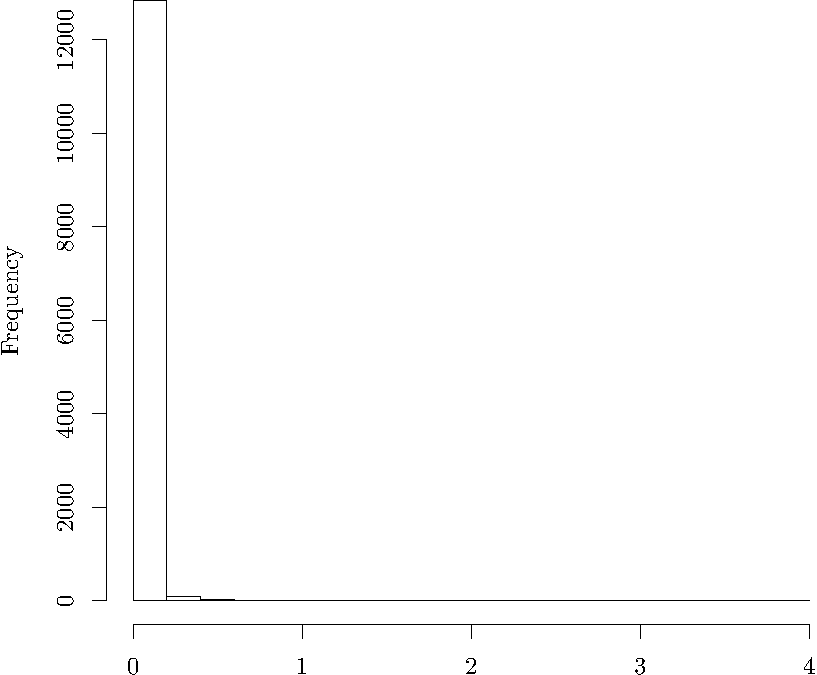
\includegraphics[width=\maxwidth]{figure/07-E3-E3-summary-1} 

}


\begin{kframe}\begin{alltt}
\hlkwd{hist}\hlstd{(APGI.messina}\hlopt{@}\hlkwc{fits}\hlopt{@}\hlkwc{summary}\hlopt{$}\hlstd{margin[APGI.messina}\hlopt{@}\hlkwc{fits}\hlopt{@}\hlkwc{summary}\hlopt{$}\hlstd{passed} \hlopt{==} \hlnum{TRUE}\hlstd{],} \hlkwc{main} \hlstd{=} \hlstr{""}\hlstd{,} \hlkwc{xlab} \hlstd{=} \hlstr{""}\hlstd{)}
\end{alltt}
\end{kframe}

{\centering 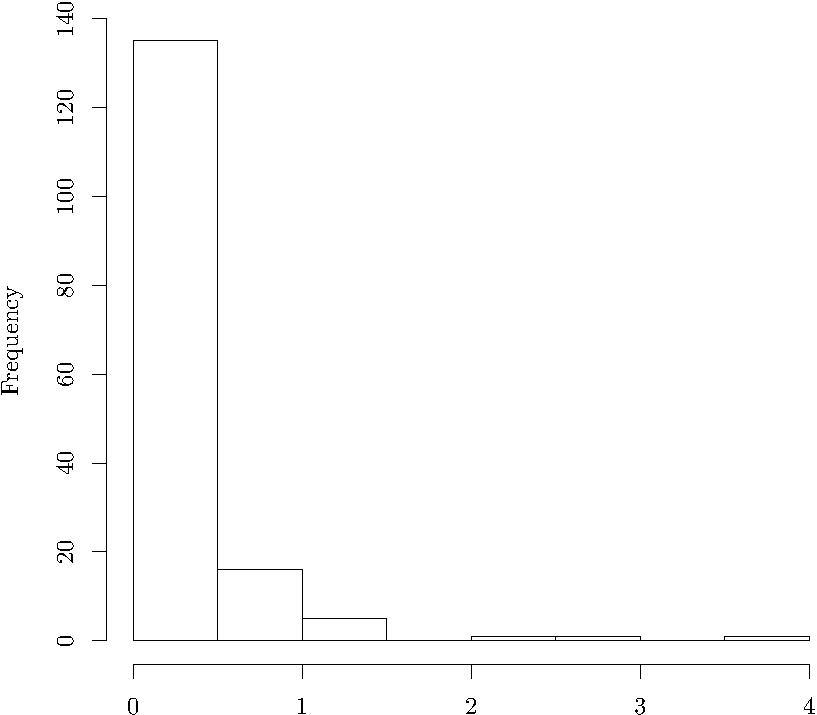
\includegraphics[width=\maxwidth]{figure/07-E3-E3-summary-2} 

}


\begin{kframe}\begin{alltt}
\hlkwd{sum}\hlstd{(APGI.messina}\hlopt{@}\hlkwc{fits}\hlopt{@}\hlkwc{summary}\hlopt{$}\hlstd{passed} \hlopt{==} \hlnum{TRUE}\hlstd{)}
\end{alltt}
\begin{verbatim}
## [1] 159
\end{verbatim}
\begin{alltt}
\hlkwd{mean}\hlstd{(APGI.messina}\hlopt{@}\hlkwc{fits}\hlopt{@}\hlkwc{summary}\hlopt{$}\hlstd{passed} \hlopt{==} \hlnum{TRUE}\hlstd{)}
\end{alltt}
\begin{verbatim}
## [1] 0.01223
\end{verbatim}
\begin{alltt}
\hlkwd{sum}\hlstd{(APGI.messina}\hlopt{@}\hlkwc{fits}\hlopt{@}\hlkwc{summary}\hlopt{$}\hlstd{margin} \hlopt{>=} \hlnum{1}\hlstd{)}
\end{alltt}
\begin{verbatim}
## [1] 11
\end{verbatim}
\begin{alltt}
\hlkwd{mean}\hlstd{(APGI.messina}\hlopt{@}\hlkwc{fits}\hlopt{@}\hlkwc{summary}\hlopt{$}\hlstd{margin} \hlopt{>=} \hlnum{1}\hlstd{)}
\end{alltt}
\begin{verbatim}
## [1] 0.0008462
\end{verbatim}
\begin{alltt}
\hlkwd{sum}\hlstd{(APGI.messina}\hlopt{@}\hlkwc{fits}\hlopt{@}\hlkwc{summary}\hlopt{$}\hlstd{margin} \hlopt{>=} \hlnum{1} \hlopt{&} \hlstd{APGI.messina}\hlopt{@}\hlkwc{fits}\hlopt{@}\hlkwc{summary}\hlopt{$}\hlstd{passed} \hlopt{==} \hlnum{TRUE}\hlstd{)}
\end{alltt}
\begin{verbatim}
## [1] 8
\end{verbatim}
\begin{alltt}
\hlkwd{mean}\hlstd{(APGI.messina}\hlopt{@}\hlkwc{fits}\hlopt{@}\hlkwc{summary}\hlopt{$}\hlstd{margin} \hlopt{>=} \hlnum{1} \hlopt{&} \hlstd{APGI.messina}\hlopt{@}\hlkwc{fits}\hlopt{@}\hlkwc{summary}\hlopt{$}\hlstd{passed} \hlopt{==} \hlnum{TRUE}\hlstd{)}
\end{alltt}
\begin{verbatim}
## [1] 0.0006154
\end{verbatim}
\begin{alltt}
\hlkwd{hist}\hlstd{(}\hlkwd{sapply}\hlstd{(APGI.maxstat,} \hlkwa{function}\hlstd{(}\hlkwc{x}\hlstd{) x}\hlopt{$}\hlstd{p.value),} \hlkwc{main} \hlstd{=} \hlstr{""}\hlstd{,} \hlkwc{xlab} \hlstd{=} \hlstr{""}\hlstd{)}
\end{alltt}
\end{kframe}

{\centering 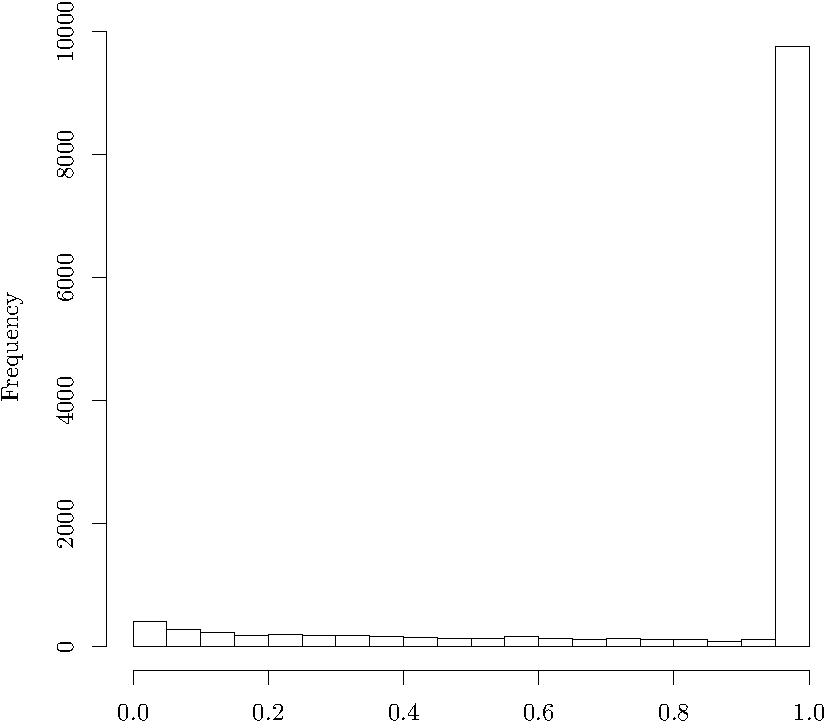
\includegraphics[width=\maxwidth]{figure/07-E3-E3-summary-3} 

}


\begin{kframe}\begin{alltt}
\hlkwd{hist}\hlstd{(}\hlkwd{log10}\hlstd{(}\hlkwd{sapply}\hlstd{(APGI.maxstat,} \hlkwa{function}\hlstd{(}\hlkwc{x}\hlstd{) x}\hlopt{$}\hlstd{p.value)),} \hlkwc{main} \hlstd{=} \hlstr{""}\hlstd{,} \hlkwc{xlab} \hlstd{=} \hlstr{""}\hlstd{)}
\end{alltt}
\end{kframe}

{\centering 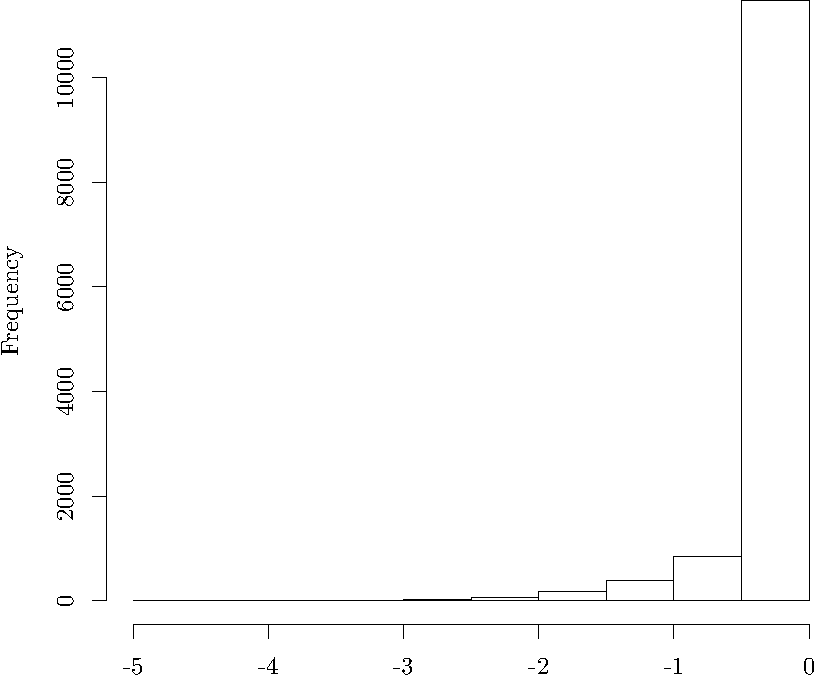
\includegraphics[width=\maxwidth]{figure/07-E3-E3-summary-4} 

}


\begin{kframe}\begin{alltt}
\hlkwd{sum}\hlstd{(}\hlkwd{sapply}\hlstd{(APGI.maxstat,} \hlkwa{function}\hlstd{(}\hlkwc{x}\hlstd{) x}\hlopt{$}\hlstd{p.value)} \hlopt{<} \hlnum{0.05}\hlstd{,} \hlkwc{na.rm} \hlstd{=} \hlnum{TRUE}\hlstd{)}
\end{alltt}
\begin{verbatim}
## [1] 413
\end{verbatim}
\begin{alltt}
\hlkwd{sum}\hlstd{(}\hlkwd{sapply}\hlstd{(APGI.maxstat,} \hlkwa{function}\hlstd{(}\hlkwc{x}\hlstd{) x}\hlopt{$}\hlstd{p.value)} \hlopt{<} \hlnum{0.05}\hlstd{,} \hlkwc{na.rm} \hlstd{=} \hlnum{TRUE}\hlstd{)} \hlopt{/} \hlkwd{length}\hlstd{(APGI.maxstat)}
\end{alltt}
\begin{verbatim}
## [1] 0.03177
\end{verbatim}
\begin{alltt}
\hlstd{APGI.messina}
\end{alltt}
\begin{verbatim}
## An object of class MessinaSurvResult
## 
## Problem type:survival
## Parameters:
##   An object of class MessinaParameters
##   13000 features, 110 samples.
##   Objective type: survival [messinaSurvObj.CoxCoef(coxcoef_threshold = 0.693)].
##   Minimum group fraction: 0.1
##   Training fraction: 0.8
##   Number of bootstraps: 50
##   Random seed: 20150321
## 
## Summary of results:
##   An object of class MessinaFits
##   159 / 13000 features passed performance requirements (1.22%)
##   Top features:
##         Passed Requirements Classifier Type Threshold Value Direction
## KRT6A                  TRUE       Threshold           9.503         1
## ANGPTL4                TRUE       Threshold           8.900         1
## KRT6C                  TRUE       Threshold           7.458         1
## IGFBP1                 TRUE       Threshold           7.070         1
## FGG                    TRUE       Threshold           8.585         1
## LYNX1                  TRUE       Threshold           7.020         1
## PPY                    TRUE       Threshold          11.931        -1
## LOX                    TRUE       Threshold           7.686         1
## DCBLD2                 TRUE       Threshold          10.959         1
## CDA                    TRUE       Threshold           8.205         1
##         Margin
## KRT6A   3.9988
## ANGPTL4 2.7155
## KRT6C   2.3334
## IGFBP1  1.4736
## FGG     1.3648
## LYNX1   1.3442
## PPY     1.0981
## LOX     1.0514
## DCBLD2  0.9851
## CDA     0.9712
\end{verbatim}
\end{kframe}
\end{knitrout}


\begin{knitrout}
\definecolor{shadecolor}{rgb}{0.969, 0.969, 0.969}\color{fgcolor}\begin{kframe}
\begin{alltt}
\hlstd{comb.feats} \hlkwb{=} \hlkwd{data.frame}\hlstd{(}\hlkwc{symbol} \hlstd{=} \hlkwd{intersect}\hlstd{(GSE28735.feats}\hlopt{$}\hlstd{Gene.symbol, TCGA.feats}\hlopt{$}\hlstd{symbol))}
\hlstd{comb.x} \hlkwb{=} \hlkwd{cbind}\hlstd{(GSE28735.x[}\hlkwd{match}\hlstd{(comb.feats}\hlopt{$}\hlstd{symbol, GSE28735.feats}\hlopt{$}\hlstd{Gene.symbol),], TCGA.x[}\hlkwd{match}\hlstd{(comb.feats}\hlopt{$}\hlstd{symbol, TCGA.feats}\hlopt{$}\hlstd{symbol),])}
\hlstd{comb.y} \hlkwb{=} \hlkwd{Surv}\hlstd{(}\hlkwd{c}\hlstd{(GSE28735.y[,}\hlnum{1}\hlstd{]}\hlopt{/}\hlnum{12}\hlopt{*}\hlnum{365.25}\hlstd{, TCGA.y[,}\hlnum{1}\hlstd{]),} \hlkwd{c}\hlstd{(GSE28735.y[,}\hlnum{2}\hlstd{], TCGA.y[,}\hlnum{2}\hlstd{]))}
\end{alltt}
\end{kframe}
\end{knitrout}


\begin{knitrout}
\definecolor{shadecolor}{rgb}{0.969, 0.969, 0.969}\color{fgcolor}\begin{kframe}
\begin{alltt}
\hlkwd{print}\hlstd{(}\hlkwd{dim}\hlstd{(APGI.x))}
\end{alltt}
\begin{verbatim}
## [1] 13000   110
\end{verbatim}
\begin{alltt}
\hlkwd{print}\hlstd{(}\hlkwd{dim}\hlstd{(GSE28735.x))}
\end{alltt}
\begin{verbatim}
## [1] 4022   42
\end{verbatim}
\begin{alltt}
\hlkwd{print}\hlstd{(}\hlkwd{dim}\hlstd{(GSE21501.x))}
\end{alltt}
\begin{verbatim}
## [1] 3908  102
\end{verbatim}
\begin{alltt}
\hlkwd{print}\hlstd{(}\hlkwd{dim}\hlstd{(TCGA.x))}
\end{alltt}
\begin{verbatim}
## [1] 20502    58
\end{verbatim}
\begin{alltt}
\hlkwd{print}\hlstd{(}\hlkwd{dim}\hlstd{(comb.x))}
\end{alltt}
\begin{verbatim}
## [1] 3742  100
\end{verbatim}
\begin{alltt}
\hlkwd{print}\hlstd{(}\hlkwd{length}\hlstd{(}\hlkwd{intersect}\hlstd{(APGI.feats}\hlopt{$}\hlstd{symbol, GSE28735.feats}\hlopt{$}\hlstd{Gene.symbol)))}
\end{alltt}
\begin{verbatim}
## [1] 2899
\end{verbatim}
\begin{alltt}
\hlkwd{print}\hlstd{(}\hlkwd{length}\hlstd{(}\hlkwd{intersect}\hlstd{(APGI.feats}\hlopt{$}\hlstd{symbol, GSE21501.feats}\hlopt{$}\hlstd{Gene.symbol)))}
\end{alltt}
\begin{verbatim}
## [1] 2545
\end{verbatim}
\begin{alltt}
\hlkwd{print}\hlstd{(}\hlkwd{length}\hlstd{(}\hlkwd{intersect}\hlstd{(APGI.feats}\hlopt{$}\hlstd{symbol, TCGA.feats}\hlopt{$}\hlstd{symbol)))}
\end{alltt}
\begin{verbatim}
## [1] 11936
\end{verbatim}
\begin{alltt}
\hlkwd{print}\hlstd{(}\hlkwd{length}\hlstd{(}\hlkwd{intersect}\hlstd{(APGI.feats}\hlopt{$}\hlstd{symbol, comb.feats}\hlopt{$}\hlstd{symbol)))}
\end{alltt}
\begin{verbatim}
## [1] 2889
\end{verbatim}
\end{kframe}
\end{knitrout}


\begin{knitrout}
\definecolor{shadecolor}{rgb}{0.969, 0.969, 0.969}\color{fgcolor}\begin{kframe}
\begin{alltt}
\hlstd{doValidation} \hlkwb{=} \hlkwa{function}\hlstd{(}\hlkwc{train.features}\hlstd{,} \hlkwc{train.x}\hlstd{,} \hlkwc{train.threshold}\hlstd{,} \hlkwc{train.merit}\hlstd{,} \hlkwc{min_merit}\hlstd{,} \hlkwc{test.features}\hlstd{,} \hlkwc{test.x}\hlstd{,} \hlkwc{test.y}\hlstd{)}
\hlstd{\{}
        \hlkwd{require}\hlstd{(robustbase)}

        \hlstd{sel.merit} \hlkwb{=} \hlstd{train.merit} \hlopt{>=} \hlstd{min_merit}
        \hlstd{sel.val_avail} \hlkwb{=} \hlstd{train.features} \hlopt \hlstd{test.features}
        \hlstd{sel} \hlkwb{=} \hlstd{sel.merit} \hlopt{&} \hlstd{sel.val_avail}
        \hlkwa{if} \hlstd{(}\hlopt{!}\hlkwd{all}\hlstd{(sel.merit)} \hlopt{&& !}\hlkwd{all}\hlstd{(}\hlopt{!}\hlstd{sel.merit)} \hlopt{&& !}\hlkwd{all}\hlstd{(sel.val_avail)} \hlopt{&& !}\hlkwd{all}\hlstd{(}\hlopt{!}\hlstd{sel.val_avail))}
        \hlstd{\{}
                \hlkwd{print}\hlstd{(}\hlkwd{fisher.test}\hlstd{(}\hlkwd{table}\hlstd{(sel.merit, sel.val_avail)))}
        \hlstd{\}}

        \hlstd{val.train.features} \hlkwb{=} \hlstd{train.features[sel]}
        \hlstd{val.train.x} \hlkwb{=} \hlstd{train.x[sel,,}\hlkwc{drop}\hlstd{=}\hlnum{FALSE}\hlstd{]}
        \hlstd{val.train.threshold} \hlkwb{=} \hlstd{train.threshold[sel]}
        \hlstd{val.train.merit} \hlkwb{=} \hlstd{train.merit[sel]}
        \hlstd{val.perm} \hlkwb{=} \hlkwd{match}\hlstd{(val.train.features, test.features)}
        \hlstd{val.test.features} \hlkwb{=} \hlstd{test.features[val.perm]}
        \hlstd{val.test.x} \hlkwb{=} \hlstd{test.x[val.perm,,}\hlkwc{drop}\hlstd{=}\hlnum{FALSE}\hlstd{]}

        \hlkwd{stopifnot}\hlstd{(val.test.features} \hlopt{==} \hlstd{val.train.features)}

        \hlcom{# Translate the threshold on the training x to an approximate equivalent}
        \hlcom{# on the test x, by normalization}
        \hlstd{locscale.train} \hlkwb{=} \hlkwd{apply}\hlstd{(val.train.x,} \hlnum{1}\hlstd{,} \hlkwa{function}\hlstd{(}\hlkwc{x}\hlstd{)} \hlkwd{scaleTau2}\hlstd{(x[}\hlopt{!}\hlkwd{is.na}\hlstd{(x)],} \hlkwc{mu.too} \hlstd{=} \hlnum{TRUE}\hlstd{))}
        \hlstd{loc.train} \hlkwb{=} \hlstd{locscale.train[}\hlnum{1}\hlstd{,]}
        \hlstd{scale.train} \hlkwb{=} \hlstd{locscale.train[}\hlnum{2}\hlstd{,]}

        \hlstd{locscale.test} \hlkwb{=} \hlkwd{apply}\hlstd{(val.test.x,} \hlnum{1}\hlstd{,} \hlkwa{function}\hlstd{(}\hlkwc{x}\hlstd{)} \hlkwd{scaleTau2}\hlstd{(x[}\hlopt{!}\hlkwd{is.na}\hlstd{(x)],} \hlkwc{mu.too} \hlstd{=} \hlnum{TRUE}\hlstd{))}
        \hlstd{loc.test} \hlkwb{=} \hlstd{locscale.test[}\hlnum{1}\hlstd{,]}
        \hlstd{scale.test} \hlkwb{=} \hlstd{locscale.test[}\hlnum{2}\hlstd{,]}

        \hlstd{val.test.threshold} \hlkwb{=} \hlstd{(val.train.threshold} \hlopt{-} \hlstd{loc.train)} \hlopt{/} \hlstd{scale.train} \hlopt{*} \hlstd{scale.test} \hlopt{+} \hlstd{loc.test}

        \hlstd{val.chisq} \hlkwb{=} \hlkwd{mapply}\hlstd{(}\hlkwa{function}\hlstd{(}\hlkwc{row_index}\hlstd{,} \hlkwc{threshold}\hlstd{) \{}
                \hlkwa{if} \hlstd{(}\hlkwd{is.na}\hlstd{(threshold))           \{} \hlkwd{return}\hlstd{(}\hlnum{NA}\hlstd{) \}}
                \hlstd{x} \hlkwb{=} \hlstd{val.test.x[row_index,]}
                \hlstd{xd} \hlkwb{=} \hlstd{x} \hlopt{>} \hlstd{threshold}
                \hlstd{xd} \hlkwb{=} \hlstd{xd[}\hlopt{!}\hlkwd{is.na}\hlstd{(xd)]}
                \hlkwa{if} \hlstd{(}\hlkwd{length}\hlstd{(xd)} \hlopt{==} \hlnum{0} \hlopt{||} \hlkwd{all}\hlstd{(xd)} \hlopt{||} \hlkwd{all}\hlstd{(}\hlopt{!}\hlstd{xd))     \{} \hlkwd{return}\hlstd{(}\hlnum{NA}\hlstd{) \}}
                \hlstd{fit} \hlkwb{=} \hlkwd{survdiff}\hlstd{(test.y} \hlopt{~} \hlstd{xd)}
                \hlstd{fit}\hlopt{$}\hlstd{chisq}
        \hlstd{\},} \hlnum{1}\hlopt{:}\hlkwd{length}\hlstd{(val.test.threshold), val.test.threshold)}

        \hlstd{val.abs.hr} \hlkwb{=} \hlkwd{sqrt}\hlstd{(val.chisq}\hlopt{*}\hlnum{4}\hlopt{/}\hlkwd{sum}\hlstd{(test.y[,}\hlnum{2}\hlstd{]))}

        \hlstd{result} \hlkwb{=} \hlkwd{data.frame}\hlstd{(}\hlkwc{merit} \hlstd{= val.train.merit,} \hlkwc{threshold.train} \hlstd{= val.train.threshold,} \hlkwc{threshold.test} \hlstd{= val.test.threshold,} \hlkwc{chisq} \hlstd{= val.chisq,} \hlkwc{abs.hr} \hlstd{= val.abs.hr)}
        \hlkwd{rownames}\hlstd{(result)} \hlkwb{=} \hlstd{val.test.features}
        \hlstd{result} \hlkwb{=} \hlstd{result[}\hlkwd{order}\hlstd{(}\hlopt{-}\hlstd{result}\hlopt{$}\hlstd{merit),]}
        \hlstd{result}
\hlstd{\}}

\hlcom{# debug(doValidation)}
\hlstd{val.GSE28735.messina} \hlkwb{=} \hlkwd{doValidation}\hlstd{(}\hlkwd{as.character}\hlstd{(APGI.feats}\hlopt{$}\hlstd{symbol), APGI.x, APGI.messina}\hlopt{@}\hlkwc{fits}\hlopt{@}\hlkwc{summary}\hlopt{$}\hlstd{threshold, APGI.messina}\hlopt{@}\hlkwc{fits}\hlopt{@}\hlkwc{summary}\hlopt{$}\hlstd{margin} \hlopt{*} \hlstd{APGI.messina}\hlopt{@}\hlkwc{fits}\hlopt{@}\hlkwc{summary}\hlopt{$}\hlstd{passed,} \hlnum{1}\hlstd{,} \hlkwd{as.character}\hlstd{(GSE28735.feats}\hlopt{$}\hlstd{Gene.symbol), GSE28735.x, GSE28735.y)}
\end{alltt}
\begin{verbatim}
## 
## 	Fisher's Exact Test for Count Data
## 
## data:  table(sel.merit, sel.val_avail)
## p-value = 0.01671
## alternative hypothesis: true odds ratio is not equal to 1
## 95 percent confidence interval:
##   1.13 37.46
## sample estimates:
## odds ratio 
##      5.814
\end{verbatim}
\begin{alltt}
\hlstd{val.GSE28735.maxstat} \hlkwb{=} \hlkwd{doValidation}\hlstd{(}\hlkwd{as.character}\hlstd{(APGI.feats}\hlopt{$}\hlstd{symbol), APGI.x,} \hlkwd{sapply}\hlstd{(APGI.maxstat,} \hlkwa{function}\hlstd{(}\hlkwc{x}\hlstd{) x}\hlopt{$}\hlstd{threshold),} \hlopt{-}\hlkwd{log10}\hlstd{(}\hlkwd{sapply}\hlstd{(APGI.maxstat,} \hlkwa{function}\hlstd{(}\hlkwc{x}\hlstd{) x}\hlopt{$}\hlstd{p.value)),} \hlopt{-}\hlkwd{log10}\hlstd{(}\hlnum{0.05}\hlstd{),} \hlkwd{as.character}\hlstd{(GSE28735.feats}\hlopt{$}\hlstd{Gene.symbol), GSE28735.x, GSE28735.y)}
\end{alltt}
\begin{verbatim}
## 
## 	Fisher's Exact Test for Count Data
## 
## data:  table(sel.merit, sel.val_avail)
## p-value < 2.2e-16
## alternative hypothesis: true odds ratio is not equal to 1
## 95 percent confidence interval:
##  2.431 3.653
## sample estimates:
## odds ratio 
##      2.982
\end{verbatim}
\begin{alltt}
\hlstd{val.GSE21501.messina} \hlkwb{=} \hlkwd{doValidation}\hlstd{(}\hlkwd{as.character}\hlstd{(APGI.feats}\hlopt{$}\hlstd{symbol), APGI.x, APGI.messina}\hlopt{@}\hlkwc{fits}\hlopt{@}\hlkwc{summary}\hlopt{$}\hlstd{threshold, APGI.messina}\hlopt{@}\hlkwc{fits}\hlopt{@}\hlkwc{summary}\hlopt{$}\hlstd{margin} \hlopt{*} \hlstd{APGI.messina}\hlopt{@}\hlkwc{fits}\hlopt{@}\hlkwc{summary}\hlopt{$}\hlstd{passed,} \hlnum{1}\hlstd{,} \hlkwd{as.character}\hlstd{(GSE21501.feats}\hlopt{$}\hlstd{Gene.symbol), GSE21501.x, GSE21501.y)}
\end{alltt}
\begin{verbatim}
## 
## 	Fisher's Exact Test for Count Data
## 
## data:  table(sel.merit, sel.val_avail)
## p-value = 7.261e-05
## alternative hypothesis: true odds ratio is not equal to 1
## 95 percent confidence interval:
##     3.701 1290.528
## sample estimates:
## odds ratio 
##      28.83
\end{verbatim}
\begin{alltt}
\hlstd{val.GSE21501.maxstat} \hlkwb{=} \hlkwd{doValidation}\hlstd{(}\hlkwd{as.character}\hlstd{(APGI.feats}\hlopt{$}\hlstd{symbol), APGI.x,} \hlkwd{sapply}\hlstd{(APGI.maxstat,} \hlkwa{function}\hlstd{(}\hlkwc{x}\hlstd{) x}\hlopt{$}\hlstd{threshold),} \hlopt{-}\hlkwd{log10}\hlstd{(}\hlkwd{sapply}\hlstd{(APGI.maxstat,} \hlkwa{function}\hlstd{(}\hlkwc{x}\hlstd{) x}\hlopt{$}\hlstd{p.value)),} \hlopt{-}\hlkwd{log10}\hlstd{(}\hlnum{0.05}\hlstd{),} \hlkwd{as.character}\hlstd{(GSE21501.feats}\hlopt{$}\hlstd{Gene.symbol), GSE21501.x, GSE21501.y)}
\end{alltt}
\begin{verbatim}
## 
## 	Fisher's Exact Test for Count Data
## 
## data:  table(sel.merit, sel.val_avail)
## p-value = 1.805e-10
## alternative hypothesis: true odds ratio is not equal to 1
## 95 percent confidence interval:
##  1.649 2.540
## sample estimates:
## odds ratio 
##      2.051
\end{verbatim}
\begin{alltt}
\hlstd{val.TCGA.messina} \hlkwb{=} \hlkwd{doValidation}\hlstd{(}\hlkwd{as.character}\hlstd{(APGI.feats}\hlopt{$}\hlstd{symbol), APGI.x, APGI.messina}\hlopt{@}\hlkwc{fits}\hlopt{@}\hlkwc{summary}\hlopt{$}\hlstd{threshold, APGI.messina}\hlopt{@}\hlkwc{fits}\hlopt{@}\hlkwc{summary}\hlopt{$}\hlstd{margin} \hlopt{*} \hlstd{APGI.messina}\hlopt{@}\hlkwc{fits}\hlopt{@}\hlkwc{summary}\hlopt{$}\hlstd{passed,} \hlnum{1}\hlstd{,} \hlkwd{as.character}\hlstd{(TCGA.feats}\hlopt{$}\hlstd{symbol), TCGA.x, TCGA.y)}
\end{alltt}
\begin{verbatim}
## 
## 	Fisher's Exact Test for Count Data
## 
## data:  table(sel.merit, sel.val_avail)
## p-value = 1
## alternative hypothesis: true odds ratio is not equal to 1
## 95 percent confidence interval:
##  0.152   Inf
## sample estimates:
## odds ratio 
##        Inf
\end{verbatim}
\begin{alltt}
\hlstd{val.TCGA.maxstat} \hlkwb{=} \hlkwd{doValidation}\hlstd{(}\hlkwd{as.character}\hlstd{(APGI.feats}\hlopt{$}\hlstd{symbol), APGI.x,} \hlkwd{sapply}\hlstd{(APGI.maxstat,} \hlkwa{function}\hlstd{(}\hlkwc{x}\hlstd{) x}\hlopt{$}\hlstd{threshold),} \hlopt{-}\hlkwd{log10}\hlstd{(}\hlkwd{sapply}\hlstd{(APGI.maxstat,} \hlkwa{function}\hlstd{(}\hlkwc{x}\hlstd{) x}\hlopt{$}\hlstd{p.value)),} \hlopt{-}\hlkwd{log10}\hlstd{(}\hlnum{0.05}\hlstd{),} \hlkwd{as.character}\hlstd{(TCGA.feats}\hlopt{$}\hlstd{symbol), TCGA.x, TCGA.y)}
\end{alltt}
\begin{verbatim}
## 
## 	Fisher's Exact Test for Count Data
## 
## data:  table(sel.merit, sel.val_avail)
## p-value = 0.08234
## alternative hypothesis: true odds ratio is not equal to 1
## 95 percent confidence interval:
##  0.961 2.318
## sample estimates:
## odds ratio 
##       1.46
\end{verbatim}
\begin{alltt}
\hlstd{val.comb.messina} \hlkwb{=} \hlkwd{doValidation}\hlstd{(}\hlkwd{as.character}\hlstd{(APGI.feats}\hlopt{$}\hlstd{symbol), APGI.x, APGI.messina}\hlopt{@}\hlkwc{fits}\hlopt{@}\hlkwc{summary}\hlopt{$}\hlstd{threshold, APGI.messina}\hlopt{@}\hlkwc{fits}\hlopt{@}\hlkwc{summary}\hlopt{$}\hlstd{margin} \hlopt{*} \hlstd{APGI.messina}\hlopt{@}\hlkwc{fits}\hlopt{@}\hlkwc{summary}\hlopt{$}\hlstd{passed,} \hlnum{1}\hlstd{,} \hlkwd{as.character}\hlstd{(comb.feats}\hlopt{$}\hlstd{symbol), comb.x, comb.y)}
\end{alltt}
\begin{verbatim}
## 
## 	Fisher's Exact Test for Count Data
## 
## data:  table(sel.merit, sel.val_avail)
## p-value = 0.01646
## alternative hypothesis: true odds ratio is not equal to 1
## 95 percent confidence interval:
##   1.136 37.631
## sample estimates:
## odds ratio 
##       5.84
\end{verbatim}
\begin{alltt}
\hlstd{val.comb.maxstat} \hlkwb{=} \hlkwd{doValidation}\hlstd{(}\hlkwd{as.character}\hlstd{(APGI.feats}\hlopt{$}\hlstd{symbol), APGI.x,} \hlkwd{sapply}\hlstd{(APGI.maxstat,} \hlkwa{function}\hlstd{(}\hlkwc{x}\hlstd{) x}\hlopt{$}\hlstd{threshold),} \hlopt{-}\hlkwd{log10}\hlstd{(}\hlkwd{sapply}\hlstd{(APGI.maxstat,} \hlkwa{function}\hlstd{(}\hlkwc{x}\hlstd{) x}\hlopt{$}\hlstd{p.value)),} \hlopt{-}\hlkwd{log10}\hlstd{(}\hlnum{0.05}\hlstd{),} \hlkwd{as.character}\hlstd{(comb.feats}\hlopt{$}\hlstd{symbol), comb.x, comb.y)}
\end{alltt}
\begin{verbatim}
## 
## 	Fisher's Exact Test for Count Data
## 
## data:  table(sel.merit, sel.val_avail)
## p-value < 2.2e-16
## alternative hypothesis: true odds ratio is not equal to 1
## 95 percent confidence interval:
##  2.418 3.633
## sample estimates:
## odds ratio 
##      2.965
\end{verbatim}
\begin{alltt}
\hlkwd{print}\hlstd{(val.GSE28735.messina)}
\end{alltt}
\begin{verbatim}
##         merit threshold.train threshold.test  chisq abs.hr
## KRT6A   3.999           9.503          4.754 1.6382 0.4753
## ANGPTL4 2.716           8.900          3.754 0.6709 0.3042
## FGG     1.365           8.585         13.796     NA     NA
## PPY     1.098          11.931          4.068 2.5368 0.5915
## LOX     1.051           7.686          6.841 0.4943 0.2611
\end{verbatim}
\begin{alltt}
\hlkwd{print}\hlstd{(val.GSE21501.messina)}
\end{alltt}
\begin{verbatim}
##         merit threshold.train threshold.test  chisq  abs.hr
## KRT6A   3.999           9.503         3.3849 0.2333 0.11891
## ANGPTL4 2.716           8.900         0.7529 0.1246 0.08691
## KRT6C   2.333           7.458        40.3387     NA      NA
## IGFBP1  1.474           7.070        -4.0458 2.3645 0.37856
## FGG     1.365           8.585         9.7976     NA      NA
## PPY     1.098          11.931         3.8380 0.3419 0.14395
## LOX     1.051           7.686        -0.5062 0.1867 0.10636
\end{verbatim}
\begin{alltt}
\hlkwd{print}\hlstd{(val.TCGA.messina)}
\end{alltt}
\begin{verbatim}
##         merit threshold.train threshold.test  chisq abs.hr
## KRT6A   3.999           9.503          3.656 1.4483 0.5838
## ANGPTL4 2.716           8.900          3.336 0.2310 0.2331
## KRT6C   2.333           7.458         16.773     NA     NA
## IGFBP1  1.474           7.070          3.788     NA     NA
## FGG     1.365           8.585         10.219     NA     NA
## LYNX1   1.344           7.020          3.998     NA     NA
## PPY     1.098          11.931          3.969 0.3139 0.2718
## LOX     1.051           7.686          3.602 0.3011 0.2662
\end{verbatim}
\begin{alltt}
\hlkwd{print}\hlstd{(val.comb.messina)}
\end{alltt}
\begin{verbatim}
##         merit threshold.train threshold.test    chisq  abs.hr
## KRT6A   3.999           9.503          4.029 0.039744 0.05879
## ANGPTL4 2.716           8.900          3.359 0.066278 0.07592
## FGG     1.365           8.585         12.497       NA      NA
## PPY     1.098          11.931          4.015 1.971306 0.41403
## LOX     1.051           7.686          3.810 0.003568 0.01761
\end{verbatim}
\begin{alltt}
\hlkwd{print}\hlstd{(val.GSE28735.maxstat)}
\end{alltt}
\begin{verbatim}
##            merit threshold.train threshold.test     chisq  abs.hr
## ANGPTL4    4.835           8.356          3.527 1.217e+00 0.40975
## KRT6A      4.450           8.915          4.503 2.180e+00 0.54832
## LOX        4.225           7.502          6.609 5.419e-01 0.27339
## PYGL       3.837           8.829          7.074 2.251e+00 0.55715
## ST6GAL1    3.803           9.542          6.145 1.230e+00 0.41191
## FAM189A2   3.630           6.455          4.052 3.197e-03 0.02100
## KLHL5      3.511           8.978          6.464 2.728e+00 0.61346
## ADM        3.394           8.820          4.730 1.088e+00 0.38741
## E2F7       3.373           6.507          3.854 4.938e+00 0.82532
## SMOX       3.165           7.190          4.852 2.650e-02 0.06045
## KIF20A     3.123           7.250          3.584 2.396e+00 0.57493
## CAPN6      3.073           6.516          4.094 7.537e-01 0.32243
## IL20RB     2.994           6.505          3.492 6.901e-01 0.30852
## P4HA1      2.882           9.080          7.426 3.618e-02 0.07064
## FYN        2.854           8.079          6.086 5.064e-01 0.26428
## AURKA      2.850           7.727          3.628 5.199e-01 0.26779
## TCEA3      2.791           8.955          4.898 3.547e+00 0.69941
## LOXL4      2.778           7.628          3.985 4.353e-03 0.02450
## LDHA       2.744          11.922          9.716 6.056e-01 0.28901
## CKAP2L     2.693           7.047          3.898 3.238e+00 0.66834
## PPY        2.628          11.966          4.074 2.537e+00 0.59153
## TREM1      2.588           6.546          5.146 3.641e-01 0.22411
## PLOD1      2.541          10.492          5.802 6.070e-02 0.09150
## CDC20      2.506           8.806          4.385 7.903e-01 0.33017
## PFKP       2.483           9.183          5.636 7.701e-02 0.10307
## ERRFI1     2.364          10.222          8.463 2.657e-02 0.06054
## RGS5       2.303           8.665          6.941 1.157e-01 0.12634
## TPX2       2.283           7.213          4.613 2.342e+00 0.56834
## P4HA2      2.267           9.209          6.579 2.345e+00 0.56868
## SLC15A1    2.242           6.716          5.053 4.828e-01 0.25805
## DPY19L1    2.227           9.183          6.364 3.403e-02 0.06851
## MME        2.227           6.441          4.645 1.425e-01 0.14019
## ATF7IP2    2.212           7.139          5.793 4.623e-02 0.07986
## PAEP       2.186           6.304          5.022 2.214e-01 0.17473
## EPHX2      2.173           7.223          3.637 7.331e-01 0.31800
## KYNU       2.169           7.161          5.370 9.540e-04 0.01147
## FOXM1      2.166           6.884          4.573 5.998e+00 0.90954
## NAMPT      2.159           7.988         10.049 3.699e-01 0.22588
## PLOD2      2.155          10.451          7.593 3.300e+00 0.67467
## UPP1       2.130           9.094          4.411 1.248e+00 0.41484
## KCTD10     2.119           7.907          6.094 3.352e-04 0.00680
## ZNF185     2.105           7.420          3.933 1.060e+00 0.38235
## EDIL3      2.105           6.400          8.217 5.409e-03 0.02731
## NEK2       2.103           8.167          4.426 5.032e-01 0.26344
## LCP1       2.100           8.702          6.629 6.413e+00 0.94049
## GAPDH      2.086          11.336          9.814 1.951e+00 0.51882
## ARSD       2.085           9.970          6.440 2.866e+00 0.62874
## KIF2C      2.080           6.839          3.953 3.629e+00 0.70749
## ENO2       2.069           7.557          5.422 3.748e-02 0.07190
## COL12A1    2.052           8.689          8.314 5.723e-02 0.08884
## VSNL1      2.052           6.712          4.221 2.337e-03 0.01796
## ENTHD1     2.044           6.345          3.130 1.851e-01 0.15977
## CADPS2     2.043           7.892          5.795 3.026e+00 0.64603
## ASPM       1.993           7.916          5.271 9.366e-02 0.11366
## ASAP1      1.993           9.917          7.260 4.509e-02 0.07886
## SPATA18    1.952           7.197          5.264 2.207e+00 0.55180
## KRT18      1.943          12.487          7.917 6.325e-01 0.29538
## POLQ       1.938           6.758          3.609 5.093e+00 0.83813
## FAM3D      1.933           9.474          6.136 2.076e+00 0.53516
## CD109      1.929           6.370          5.959 2.207e-01 0.17446
## UBE2C      1.927           9.305          5.228 1.843e+00 0.50417
## OCLN       1.922           7.722          7.186 5.277e-01 0.26980
## WNK2       1.915           6.293          3.922 2.774e+00 0.61854
## TGFBI      1.912          12.180          8.229 2.750e+00 0.61587
## SPOCK1     1.903           8.915          5.387 7.009e+00 0.98323
## CD300A     1.885           6.707          5.248 1.331e-01 0.13548
## RAVER2     1.856           7.583          5.856 7.799e-01 0.32798
## P2RY8      1.856           7.349          4.024 1.079e-02 0.03858
## A4GNT      1.846           6.439          3.549 1.023e+00 0.37571
## RIMKLB     1.825           7.221          6.093 7.238e-03 0.03160
## ADAM23     1.824           6.394          4.155 7.598e-03 0.03237
## FST        1.820           7.155          4.557 1.088e+00 0.38730
## CA8        1.819           6.429          3.264 1.650e+00 0.47710
## CEP55      1.819           7.985          4.831 1.431e+00 0.44426
## IL1A       1.813           6.266          2.599 1.460e-01 0.14191
## ANLN       1.811           7.020          4.871 3.439e+00 0.68875
## DCBLD2     1.806          10.689          8.544 7.788e+00 1.03647
## PLA2G10    1.795           9.726          4.000 4.374e+00 0.77673
## KLHL13     1.791           6.430          3.543 6.677e-01 0.30348
## STAG3L4    1.784           6.532          4.970 3.087e-01 0.20636
## GOLM1      1.777           6.547          8.986        NA      NA
## F3         1.770           9.228          7.930 4.135e-02 0.07552
## NTS        1.760           6.317          2.643 1.702e+00 0.48451
## TPI1       1.759          10.890          6.342 4.913e-01 0.26033
## PTGES      1.757           7.540          4.722 7.838e-06 0.00104
## IGKV1ORY-1 1.755          11.809          7.375 2.201e-03 0.01742
## SNAI2      1.753           8.469          6.705 7.687e-02 0.10297
## NFIA       1.727           7.914          5.845 1.255e+00 0.41606
## COL7A1     1.726           8.066          4.932 2.645e+00 0.60395
## FGD6       1.724           6.426          6.617 9.292e-01 0.35800
## MCM4       1.721           7.948          5.209 1.214e+00 0.40916
## TUBA1C     1.720          11.899          6.920 1.285e-02 0.04210
## MELK       1.713           7.288          4.752 2.117e+00 0.54039
## C5orf46    1.700           6.858          2.836        NA      NA
## COL17A1    1.700          10.742          6.042 7.886e-01 0.32980
## PDLIM7     1.691           8.030          6.383 6.057e-01 0.28905
## PTTG1      1.674           9.067          4.939 1.004e+00 0.37213
## DSG2       1.663          10.999          7.174 6.084e+00 0.91609
## COL1A2     1.658          12.989         11.330 1.470e+00 0.45034
## SYNE2      1.657           8.782          7.637 1.589e-01 0.14803
## SERPINH1   1.646          10.187          6.735 2.134e+00 0.54256
## PHLDA1     1.643           9.269          6.348 1.132e+00 0.39517
## CTSE       1.642          11.677          9.666 1.154e+00 0.39904
## ADH1A      1.635           8.432          4.306 3.482e+00 0.69297
## WEE1       1.635           7.480          7.084 1.675e+00 0.48070
## CHEK1      1.623           6.501          4.403 2.718e+00 0.61232
## GSDMC      1.618           6.409          3.565 4.329e+00 0.77272
## SLC2A1     1.615          10.218          7.422 3.749e-03 0.02274
## SERPINB3   1.614           6.324          2.770 1.020e-02 0.03752
## DHRS9      1.609           8.430          4.046 2.091e-01 0.16984
## PPP1R3C    1.597           8.282          5.976 3.812e+00 0.72507
## FLRT3      1.596           9.224          5.713 3.404e+00 0.68522
## CCNB2      1.594           7.685          4.108 1.338e+00 0.42967
## CORO1A     1.593           8.375          5.960 4.792e-03 0.02571
## RHOF       1.591           6.800          4.881 5.617e-01 0.27835
## GRAMD3     1.587           7.707          5.612 7.763e-03 0.03272
## IL33       1.583           7.299          4.397 2.122e-03 0.01711
## AQP1       1.577           7.146          5.848 7.817e-02 0.10384
## VEGFA      1.573           7.090          6.212 1.095e-02 0.03887
## ANGPTL2    1.563           9.897          5.866 1.308e+00 0.42483
## SEMA4A     1.562           7.304          4.697 1.226e-01 0.13004
## GCNT1      1.562           8.263          6.462 2.802e-01 0.19661
## CCL19      1.560           9.155          6.111 2.032e-01 0.16742
## CACHD1     1.555           6.709          5.075 4.289e-03 0.02432
## NCAPG      1.544           7.323          5.149 4.495e-01 0.24900
## FCGR2B     1.536           7.007          4.506 2.784e-02 0.06197
## BOC        1.528           6.805          5.509 3.207e+00 0.66507
## CNIH3      1.513           6.461          4.149 9.764e-01 0.36699
## IL1R2      1.508           8.252          5.522 3.305e+00 0.67523
## ITGA5      1.505           8.100          5.330 7.701e-02 0.10307
## ITM2A      1.504           9.660          5.222 7.935e-01 0.33084
## SLC9A9     1.502           7.348          6.777 2.790e-02 0.06203
## TM4SF19    1.496           6.269          4.532 1.245e+00 0.41442
## JAG1       1.488           9.130          8.263 4.872e+00 0.81979
## FN1        1.486           6.406         11.169 2.450e-02 0.05813
## NRP2       1.484           6.606          8.615        NA      NA
## TNNI2      1.480           6.303          4.497 3.223e-01 0.21086
## APOL1      1.469           6.456          7.103 6.062e-02 0.09144
## KANK4      1.468           7.979          4.247 2.105e-01 0.17040
## RFX2       1.463           6.427          5.086 5.510e-01 0.27568
## DSC2       1.458           6.704          7.468 8.154e+00 1.06049
## KRT17      1.449          10.862          6.923 1.492e+00 0.45370
## ANKLE2     1.448           7.795          6.781 1.866e+00 0.50736
## PRC1       1.445           8.324          5.413 2.803e+00 0.62174
## PPP2R2C    1.443           6.859          3.662 4.825e+00 0.81578
## KIF18A     1.440           6.472          3.550 1.717e+00 0.48658
## NDRG2      1.438           8.691          6.250 2.768e+00 0.61792
## LONRF2     1.437           6.411          4.445 4.865e-01 0.25904
## SEMA3A     1.432           7.328          6.924 1.541e+00 0.46100
## ARHGAP26   1.426           6.622          7.091 3.126e+00 0.65660
## ZBED2      1.424           6.267          4.047 1.361e+00 0.43327
## PCF11      1.422           6.970          5.972 5.690e+00 0.88589
## IGJ        1.420           9.761         10.380 1.711e-02 0.04857
## RGS16      1.419           6.813          5.669 4.387e+00 0.77790
## HRASLS2    1.418           7.346          3.576 1.641e-01 0.15045
## AHCYL2     1.417           8.620          7.190 4.483e+00 0.78637
## TLE4       1.417           8.089          5.644 1.763e-02 0.04932
## CDA        1.416           6.859          4.461 1.855e-01 0.15997
## DNASE1     1.415           6.346          3.864 6.021e-01 0.28818
## DKK1       1.413           9.728          5.287 1.032e+00 0.37731
## CD38       1.405           7.104          6.298 7.484e-01 0.32128
## MALL       1.405          10.388          6.245 3.778e-01 0.22828
## GIMAP2     1.400           7.313          5.276 2.303e+00 0.56357
## GPC3       1.399           7.457          6.106 8.675e-01 0.34592
## SH3RF1     1.391           8.535          6.363 4.798e+00 0.81349
## DUOXA2     1.384           7.261          4.065 3.746e+00 0.71877
## FRMD6      1.379           9.411          7.018 1.674e+00 0.48046
## KNTC1      1.365           7.209          5.133 2.333e+00 0.56731
## TMSB10     1.364          13.721         10.239 9.794e-01 0.36754
## KPNA2      1.356           6.543          6.121 6.968e-01 0.31002
## CST6       1.354           8.451          4.027 1.272e+00 0.41878
## CCNB1      1.353           7.364          5.563 3.176e-01 0.20931
## CD79A      1.350           7.991          4.204 1.653e+00 0.47746
## RAP1GAP    1.346           9.590          3.821 2.320e-01 0.17889
## CENPF      1.346           7.209          5.142 5.130e-01 0.26601
## SOD2       1.341           8.755          7.349        NA      NA
## MIF        1.334          12.328          7.195 2.992e-01 0.20314
## GBE1       1.331           7.564          6.499 1.296e+00 0.42285
## MEOX1      1.331           6.748          4.334 3.263e-02 0.06709
## KIF14      1.322           6.914          3.835 3.222e+00 0.66666
## TRNP1      1.319          10.665          5.963 4.984e-03 0.02622
## FGG        1.319           8.010         10.996        NA      NA
## MUC16      1.312           6.930          3.937 1.296e-01 0.13368
## DYNC2H1    1.312           7.510          6.309 4.117e+00 0.75355
## MMP10      1.307           6.412          2.984 6.057e-01 0.28904
## LETM2      1.306           6.642          4.413 6.681e-01 0.30356
\end{verbatim}
\begin{alltt}
\hlkwd{print}\hlstd{(val.GSE21501.maxstat)}
\end{alltt}
\begin{verbatim}
##          merit threshold.train threshold.test     chisq   abs.hr
## ANGPTL4  4.835           8.356        0.19587 6.865e-01 0.203971
## KRT6A    4.450           8.915        2.97484 2.615e-02 0.039811
## LOX      4.225           7.502       -0.79221 1.058e+00 0.253245
## KRT6C    4.215           6.392        5.59238        NA       NA
## ST6GAL1  3.803           9.542        0.78319 5.739e-01 0.186504
## FAM189A2 3.630           6.455        0.28808 7.248e-01 0.209584
## ADM      3.394           8.820       -1.66023 7.681e+00 0.682307
## E2F7     3.373           6.507       -2.26972 1.101e+01 0.816993
## CAPN6    3.073           6.516        0.58777 1.934e+00 0.342376
## IL20RB   2.994           6.505        0.27819 2.890e+00 0.418499
## FGF13    2.837           6.400       -0.33980 2.197e+00 0.364889
## TCEA3    2.791           8.955        0.67789 4.561e+00 0.525732
## LOXL4    2.778           7.628        0.96728 4.499e-01 0.165118
## TMEM26   2.688           6.692        0.77037 4.695e-02 0.053341
## BIRC5    2.643           7.334       -1.61111 4.021e+00 0.493655
## CD70     2.632           6.748       -0.60306 5.035e-01 0.174694
## PPY      2.628          11.966        3.85564 7.804e-01 0.217485
## TREM1    2.588           6.546        2.12235 4.167e+00 0.502511
## IGFBP1   2.466           7.076       -4.02812 1.675e+00 0.318579
## ERRFI1   2.364          10.222        0.59119 1.790e+01 1.041655
## RGS5     2.303           8.665        4.26999 5.369e+00 0.570428
## PHACTR3  2.275           6.884        1.98393 1.343e+00 0.285312
## MME      2.227           6.441       -1.58576 2.189e-01 0.115175
## PRDM16   2.206           6.605        3.97296 1.839e+00 0.333875
## PAEP     2.186           6.304        0.77117 4.242e-01 0.160333
## EPHX2    2.173           7.223        0.03016 4.564e-01 0.166306
## KYNU     2.169           7.161       -1.99673 3.795e-01 0.151662
## NAMPT    2.159           7.988        0.11528 1.970e+00 0.345539
## PLOD2    2.155          10.451        0.06961 8.655e-02 0.072425
## EDIL3    2.105           6.400        4.24471 1.304e+00 0.281169
## NEK2     2.103           8.167       -1.80395 4.750e+00 0.536570
## LCP1     2.100           8.702       -1.84614 2.896e+00 0.418967
## COL12A1  2.052           8.689        1.83301 3.053e-01 0.136032
## VSNL1    2.052           6.712       -1.64740 1.529e-01 0.096261
## ENTHD1   2.044           6.345        1.75682 2.632e-01 0.126309
## PCDH20   2.003           7.551        3.99419 1.354e+00 0.286499
## ASPM     1.993           7.916       -0.07079 1.759e+00 0.326534
## CATSPER1 1.956           6.371        0.89696 1.486e+00 0.300113
## KRT18    1.943          12.487        0.25249 1.552e+00 0.306688
## FAM3D    1.933           9.474        5.30834 6.346e+00 0.620176
## CD109    1.929           6.370       -0.49431 4.737e-01 0.169441
## UBE2C    1.927           9.305       -1.15748 2.006e+00 0.348648
## OCLN     1.922           7.722        2.27334 3.056e+00 0.430370
## TGFBI    1.912          12.180        1.17508 7.810e-02 0.068799
## SPOCK1   1.903           8.915       -0.07385 3.241e-02 0.044319
## P2RY2    1.899           6.885        2.53729 5.626e-01 0.184657
## RAVER2   1.856           7.583        0.05711 4.701e-01 0.168793
## P2RY8    1.856           7.349        0.52845 1.882e+00 0.337727
## A4GNT    1.846           6.439        3.40057 8.431e-01 0.226048
## APOA4    1.823           6.333       -1.04560 3.747e-01 0.150698
## CEP55    1.819           7.985       -0.77283 1.442e-03 0.009348
## IL1A     1.813           6.266       -0.13329 2.483e-02 0.038792
## ANLN     1.811           7.020       -2.66571 1.547e-01 0.096836
## DCBLD2   1.806          10.689        0.63766 4.607e+00 0.528400
## PLA2G10  1.795           9.726        3.52033 1.519e-01 0.095962
## GOLM1    1.777           6.547        4.36321 3.484e+00 0.459532
## F3       1.770           9.228        3.33470 7.961e-01 0.219662
## NTS      1.760           6.317       -5.02906 1.450e+00 0.296467
## SNAI2    1.753           8.469        0.96462 2.333e+00 0.376030
## COL7A1   1.726           8.066       -0.65725 1.243e+00 0.274511
## FGD6     1.724           6.426        1.00560 2.874e-02 0.041738
## NFIX     1.713           9.904        1.57937 1.036e+00 0.250572
## C5orf46  1.700           6.858        1.16807 5.466e+00 0.575554
## COL17A1  1.700          10.742        4.24593 2.682e-01 0.127500
## VSTM2L   1.679           7.078        2.67464 2.975e-01 0.134266
## COL1A2   1.658          12.989        3.96788 4.629e-03 0.016750
## SERPINH1 1.646          10.187        0.16779 4.575e+00 0.526550
## CTSE     1.642          11.677        7.26038 3.184e+00 0.439271
## TNFRSF6B 1.638           7.634        3.32680 6.004e-01 0.190757
## ADH1A    1.635           8.432        2.32552 1.282e+00 0.278749
## CHEK1    1.623           6.501       -3.47669 7.154e-02 0.065844
## SLC2A1   1.615          10.218       -0.52907 5.130e-01 0.176320
## SERPINB3 1.614           6.324        0.71096 4.767e-01 0.169980
## DHRS9    1.609           8.430        1.56562 2.307e+00 0.373911
## PPP1R3C  1.597           8.282        0.52826 8.428e-05 0.002260
## FLRT3    1.596           9.224        3.15856 2.789e+00 0.411136
## CCNB2    1.594           7.685       -0.56249 1.099e+00 0.258023
## CXCR5    1.589           6.681        7.98854        NA       NA
## IL33     1.583           7.299        4.11799 2.212e-02 0.036611
## AQP1     1.577           7.146        3.32621 1.330e-01 0.089783
## TNFRSF17 1.573           7.032       12.81828        NA       NA
## VEGFA    1.573           7.090       -0.39754 2.750e-01 0.129105
## GCNT1    1.562           8.263        1.40450 6.109e-02 0.060848
## CCL19    1.560           9.155        5.98546 9.945e-01 0.245510
## ADRA1B   1.546           6.285        0.12758 3.060e+00 0.430671
## CAV2     1.540           8.562        1.61441 2.749e+00 0.408156
## FCGR2B   1.536           7.007        1.56740 9.048e-01 0.234173
## MRAP2    1.532           7.684        0.29126 2.912e-01 0.132852
## CCL3L3   1.524           6.799        1.79960 1.696e+00 0.320563
## CNIH3    1.513           6.461        0.57543 1.041e+00 0.251233
## IL1R2    1.508           8.252        3.85019 2.006e-01 0.110265
## ITM2A    1.504           9.660       -0.78323 1.336e+00 0.284577
## SLC9A9   1.502           7.348        3.46665 9.579e-02 0.076192
## FN1      1.486           6.406        0.04531 3.830e-01 0.152356
## SOX8     1.486           7.496        0.79012 5.370e-03 0.018041
## NRP2     1.484           6.606        5.28797        NA       NA
## TNNI2    1.480           6.303       -1.30119 7.253e+00 0.662984
## HES1     1.479           8.112        1.10294 4.000e-01 0.155700
## KCNH2    1.476           6.778        0.69336 2.375e+00 0.379430
## APOL1    1.469           6.456        0.79884 2.381e-02 0.037989
## KANK4    1.468           7.979        1.54307 1.052e-01 0.079839
## KRT17    1.449          10.862        1.84873 3.034e+00 0.428807
## PPP2R2C  1.443           6.859       -0.11054 1.115e-01 0.082189
## KIF18A   1.440           6.472       -2.19452 1.770e-01 0.103563
## LONRF2   1.437           6.411       -1.25358 1.612e+00 0.312580
## SEMA3A   1.432           7.328        0.13548 6.067e-01 0.191751
## ARHGAP26 1.426           6.622        1.86500 5.095e-01 0.175719
## ZBED2    1.424           6.267        2.24266 7.387e-01 0.211587
## SPOCD1   1.422           6.904        1.25823 5.807e+00 0.593238
## IGJ      1.420           9.761        1.21379 3.078e-01 0.136571
## RGS16    1.419           6.813        1.94034 2.366e-01 0.119752
## HRASLS2  1.418           7.346        4.41621 2.843e-01 0.131273
## AHCYL2   1.417           8.620        1.74374 4.884e+00 0.544052
## DNASE1   1.415           6.346        0.03199 5.313e-02 0.056746
## DKK1     1.413           9.728        0.52018 1.947e+00 0.343491
## CD38     1.405           7.104        2.18938 7.635e-01 0.215108
## MALL     1.405          10.388        3.83833 5.231e-01 0.178049
## FGF18    1.397           6.280        1.94601 3.342e-03 0.014232
## ZNF365   1.390           7.180        2.32667 3.166e-01 0.138525
## FRMD6    1.379           9.411        1.01822 1.170e-02 0.026633
## TK1      1.375           8.114       -1.37859 4.348e+00 0.513363
## CST6     1.354           8.451        4.65564 2.530e-01 0.123838
## CD79A    1.350           7.991        2.33695 7.925e-02 0.069304
## RAP1GAP  1.346           9.590        0.53578 8.878e-03 0.023196
## CENPF    1.346           7.209       -2.07887 2.536e+00 0.392078
## SOD2     1.341           8.755       -0.40747 6.928e-01 0.204903
## MEOX1    1.331           6.748        0.96369 5.732e-01 0.186382
## KIF14    1.322           6.914       -1.85459 3.210e-01 0.139485
## TRNP1    1.319          10.665        3.20514 9.527e-04 0.007599
## FGG      1.319           8.010        6.42581        NA       NA
## CBX1     1.317           6.644        0.09649 4.679e-01 0.168403
## MUC16    1.312           6.930       -1.13833 1.513e-01 0.095769
## DYNC2H1  1.312           7.510        0.47423 6.089e-03 0.019209
## GATA6    1.310           6.470        3.72622 2.664e+00 0.401788
## MMP10    1.307           6.412        1.44298 3.202e-02 0.044051
\end{verbatim}
\begin{alltt}
\hlkwd{print}\hlstd{(val.TCGA.maxstat)}
\end{alltt}
\begin{verbatim}
##           merit threshold.train threshold.test     chisq   abs.hr
## ANGPTL4   4.835           8.356         3.2506 8.573e-02 0.142030
## B3GALTL   4.586           6.747         3.1744 4.692e-01 0.332277
## KRT6A     4.450           8.915         3.5365 2.464e+00 0.761458
## LOX       4.225           7.502         3.5709 6.397e-01 0.387968
## KRT6C     4.215           6.392         3.9993        NA       NA
## PFKFB4    4.140           7.004         3.0053 3.090e-01 0.269623
## CIDEC     3.851           7.623         3.0437 2.472e-01 0.241173
## PYGL      3.837           8.829         3.4693 2.323e+00 0.739303
## ST6GAL1   3.803           9.542         3.6540 4.597e-02 0.104006
## FAM189A2  3.630           6.455         2.8347 6.560e-01 0.392865
## RPIA      3.527           7.988         3.2886 1.041e+00 0.494966
## KLHL5     3.511           8.978         3.4314 8.833e-01 0.455900
## LYNX1     3.490           6.603         3.5629 3.300e+01 2.786522
## TRAPPC2   3.466           8.229         3.2071 5.559e-01 0.361659
## ZNF565    3.451           6.532         2.8439 9.433e-01 0.471122
## ADM       3.394           8.820         3.0578 1.290e+00 0.550837
## E2F7      3.373           6.507         2.8931 3.369e+00 0.890337
## KTI12     3.278           7.949         3.1614 1.803e+00 0.651319
## UFC1      3.264           9.787         3.5679 1.613e-01 0.194826
## HJURP     3.180           6.967         3.1594 2.203e+00 0.719982
## SMOX      3.165           7.190         3.2938 2.054e-01 0.219816
## KIF20A    3.123           7.250         3.1635 8.137e-01 0.437564
## ELMOD3    3.075           7.298         3.2690 2.506e-01 0.242803
## NACC2     3.073           6.578         2.7790 3.077e-02 0.085091
## CAPN6     3.073           6.516         3.1289 3.945e+00 0.963493
## IL20RB    2.994           6.505         2.6696 6.952e-01 0.404444
## CARHSP1   2.993          10.451         3.5607 2.610e+00 0.783592
## P4HA1     2.882           9.080         3.5537 8.216e-01 0.439679
## FYN       2.854           8.079         3.5020 2.393e-01 0.237278
## AURKA     2.850           7.727         3.1350 1.347e+00 0.562947
## FGF13     2.837           6.400         2.8910 2.202e-02 0.071977
## TCEA3     2.791           8.955         3.2703 1.672e+00 0.627186
## LOXL4     2.778           7.628         3.2741 1.007e+00 0.486752
## LDHA      2.744          11.922         3.8200 1.032e-01 0.155810
## SLAMF9    2.730           6.346         1.9189 2.350e+00 0.743553
## GOLPH3L   2.729           7.859         3.4711 1.324e-01 0.176470
## DEFB123   2.716           6.326            NaN        NA       NA
## SLC30A3   2.696           6.399         1.5633 2.190e+00 0.717762
## CKAP2L    2.693           7.047         3.0517 5.679e+00 1.155938
## TMEM26    2.688           6.692         2.8280 5.494e-05 0.003595
## BIRC5     2.643           7.334         3.1152 1.436e+00 0.581364
## IFT140    2.638           6.438         3.3541 3.296e-03 0.027850
## CD70      2.632           6.748         2.6457 3.625e-03 0.029205
## PPY       2.628          11.966         3.9751 3.139e-01 0.271774
## LRRFIP2   2.624           7.861         3.4000 5.492e-01 0.359463
## TREM1     2.588           6.546         3.0622 8.990e-01 0.459927
## LYRM1     2.548           9.343         3.2709 5.861e-03 0.037136
## PLOD1     2.541          10.492         3.6442 6.590e-01 0.393765
## ATP5O     2.538          11.228         3.6003 7.877e-01 0.430499
## CDC20     2.506           8.806         3.2186 4.668e-01 0.331426
## ARHGEF19  2.486           6.695         3.1074 2.975e+00 0.836710
## PFKP      2.483           9.183         3.5533 2.849e-01 0.258895
## AURKB     2.470           6.963         3.0300 1.073e+00 0.502561
## IGFBP1    2.466           7.076         3.7990        NA       NA
## VPS29     2.464           9.524         3.3949 1.012e-01 0.154339
## PHF21A    2.423           8.261         3.3828 1.254e-01 0.171748
## PDCD2L    2.416           7.446         2.9782 4.223e-01 0.315233
## FAH       2.413           7.260         3.2812 6.847e-02 0.126932
## PLIN3     2.391          11.237         3.6267 2.658e-01 0.250069
## SLC15A4   2.382           9.055         3.4043 1.492e+00 0.592598
## NOTCH1    2.378           7.822         3.4138 6.490e+00 1.235773
## ERRFI1    2.364          10.222         3.7131 2.452e+00 0.759630
## RFX4      2.360           6.318         0.6094 3.735e+00 0.937419
## RGS5      2.303           8.665         3.6868 2.529e+00 0.771462
## COL5A3    2.294           6.444         3.3676 2.353e+00 0.744144
## PTPRM     2.289           7.564         3.4899 1.177e+00 0.526291
## SOBP      2.285           7.318         3.2145 1.427e+00 0.579445
## TPX2      2.283           7.213         3.4056 5.839e+00 1.172127
## PHACTR3   2.275           6.884         2.7109 4.422e+00 1.020010
## P4HA2     2.267           9.209         3.5563 8.348e-01 0.443197
## IKBIP     2.252           6.947         3.3099 1.815e-01 0.206659
## DHRS11    2.249           7.620         3.0378 2.263e+00 0.729748
## SLC15A1   2.242           6.716         3.2639 2.503e-01 0.242659
## BMS1      2.234           9.010         3.4895 4.549e-02 0.103453
## DPY19L1   2.227           9.183         3.5265 1.193e-01 0.167516
## MME       2.227           6.441         3.1336 1.430e+00 0.580049
## ARMC7     2.218           7.589         3.2933 1.957e-03 0.021460
## ATF7IP2   2.212           7.139         3.2603 1.696e+00 0.631663
## PRDM16    2.206           6.605         3.2494 1.055e-01 0.157519
## TRIM54    2.197           8.060         3.1774 2.177e+00 0.715766
## PAEP      2.186           6.304         3.5895        NA       NA
## TM9SF3    2.181           9.973         3.8034 7.033e-01 0.406800
## TARBP2    2.175           6.959         3.2777 1.864e+00 0.662262
## EPHX2     2.173           7.223         3.1924 1.516e-04 0.005973
## SGSM1     2.171           6.631         2.9490 2.006e-02 0.068698
## KYNU      2.169           7.161         3.1598 8.082e-01 0.436070
## FOXM1     2.166           6.884         3.3186 3.181e-01 0.273580
## NAMPT     2.159           7.988         3.6866 5.716e-01 0.366727
## PLOD2     2.155          10.451         3.5670 2.931e-01 0.262627
## TTC13     2.144           7.827         3.3152 6.849e-01 0.401449
## UPP1      2.130           9.094         3.3237 9.579e-02 0.150132
## KCTD10    2.119           7.907         3.5420 5.250e-01 0.351483
## ZNF185    2.105           7.420         3.2864 1.071e+00 0.502018
## EDIL3     2.105           6.400         3.5273 3.943e+00 0.963201
## KCNQ3     2.104           6.635         2.5387 7.679e-01 0.425055
## NEK2      2.103           8.167         3.1637 1.973e-01 0.215456
## LCP1      2.100           8.702         3.5387 9.984e-03 0.048469
## CFL1      2.088          12.385         3.9427 4.260e-01 0.316604
## GAPDH     2.086          11.336         4.0228 1.957e+00 0.678555
## ARSD      2.085           9.970         3.6909 5.880e-01 0.371959
## PGBD3     2.085           6.454         2.9488 1.496e-01 0.187636
## KIF2C     2.080           6.839         3.2058 4.434e-01 0.322993
## ENO2      2.069           7.557         3.4295 1.791e+00 0.649226
## ABLIM1    2.063           9.734         3.6850 1.090e+00 0.506472
## RFC5      2.053           7.876         3.1563 2.165e+00 0.713759
## COL12A1   2.052           8.689         3.7775 5.110e-01 0.346739
## VSNL1     2.052           6.712         2.9368 7.472e-01 0.419295
## ENTHD1    2.044           6.345         2.9963 3.341e-01 0.280367
## CADPS2    2.043           7.892         3.3495 7.356e-02 0.131561
## GARS      2.035          10.140         3.5755 1.141e+00 0.518191
## SCYL2     2.021           8.564         3.4991 2.646e-01 0.249525
## PCDH20    2.003           7.551         3.5025        NA       NA
## ARFGAP3   2.001           8.794         3.5346 1.388e-01 0.180722
## ASPM      1.993           7.916         3.3218 6.506e+00 1.237243
## ASAP1     1.993           9.917         3.5695 1.304e+00 0.553869
## RPS4X     1.964          11.441         3.9567 9.396e-01 0.470206
## CATSPER1  1.956           6.371         2.4825 2.207e-01 0.227857
## SPATA18   1.952           7.197         3.2489 1.300e-01 0.174924
## GLOD5     1.944           6.455         2.9064        NA       NA
## KRT18     1.943          12.487         3.8944 9.596e-01 0.475165
## POLQ      1.938           6.758         2.9372 3.382e-01 0.282094
## FAM3D     1.933           9.474         3.6956 5.202e-01 0.349841
## CD109     1.929           6.370         3.4720 2.027e+00 0.690548
## UBE2C     1.927           9.305         3.2822 6.069e-01 0.377876
## OCLN      1.922           7.722         3.4377 7.736e-01 0.426651
## IRF2BP1   1.915           7.100         3.3272 1.025e-01 0.155301
## WNK2      1.915           6.293         3.3750 3.541e-01 0.288642
## TGFBI     1.912          12.180         3.8654 7.781e+00 1.353089
## RPL22     1.904           7.535         3.8000 7.946e-01 0.432385
## SPOCK1    1.903           8.915         3.5262 7.123e+00 1.294646
## ABHD5     1.902           6.876         3.3126 1.184e+00 0.527738
## P2RY2     1.899           6.885         2.9708 1.667e+00 0.626317
## GATC      1.896           6.590         2.8045 3.130e-01 0.271389
## FAIM2     1.891           6.411         3.0889 2.126e-01 0.223650
## DYNLL2    1.887           7.492         3.4929 3.124e+00 0.857392
## CD300A    1.885           6.707         3.2155 4.593e-02 0.103952
## GAB2      1.881           7.897         3.4618 2.567e+00 0.777131
## SPATS2    1.870           7.594         3.3907 3.015e+00 0.842265
## BAMBI     1.869           8.351         3.1289 8.300e-01 0.441922
## RAVER2    1.856           7.583         3.3692 4.196e-01 0.314207
## P2RY8     1.856           7.349         3.4846        NA       NA
## ACTR6     1.854           8.483         3.2930 1.554e+00 0.604611
## STAT5B    1.852           6.899         3.5432 1.469e+00 0.587841
## A4GNT     1.846           6.439         4.1193        NA       NA
## PQBP1     1.842           8.110         3.4243 2.566e-02 0.077710
## CGB5      1.839           6.293         2.1368 1.209e+00 0.533442
## TMEM91    1.839           7.342         2.8389 1.924e-02 0.067285
## SEPW1     1.835          10.598         3.7110 1.520e-01 0.189133
## EIF2AK3   1.832           7.163         3.4123 6.456e-03 0.038977
## RIMKLB    1.825           7.221         3.3330 7.642e-02 0.134092
## ADAM23    1.824           6.394         3.1013 3.619e+00 0.922777
## APOA4     1.823           6.333         1.1187 2.832e-01 0.258131
## FST       1.820           7.155         2.9354 1.577e-01 0.192604
## CA8       1.819           6.429         2.9970 4.371e-01 0.320695
## CEP55     1.819           7.985         3.2909 1.853e+00 0.660291
## IL1A      1.813           6.266         2.3296 3.748e-01 0.296967
## ANLN      1.811           7.020         3.2911 2.084e+00 0.700274
## DCBLD2    1.806          10.689         3.6675 1.241e+00 0.540286
## PLA2G10   1.795           9.726         2.9673 3.689e+00 0.931728
## KLHL13    1.791           6.430         2.8886 9.688e-01 0.477455
## ATP5G1    1.786           9.631         3.3717 1.065e-01 0.158287
## STAG3L4   1.784           6.532         2.9777 2.411e-03 0.023820
## GOLM1     1.777           6.547         3.9934 3.130e-01 0.271389
## FAM120AOS 1.776           8.186         3.4890 3.801e-01 0.299062
## OAZ1      1.771          13.408         3.8313 1.149e+00 0.519866
## F3        1.770           9.228         3.6677 1.306e-01 0.175272
## SSBP1     1.769          10.404         3.4807 4.902e+00 1.074000
## CDK2      1.768           7.675         3.3169 4.595e+00 1.039748
## NTS       1.760           6.317         2.1570 1.333e-01 0.177128
## EXOSC8    1.760           8.069         3.2073 2.864e+00 0.820929
## TPI1      1.759          10.890         3.7702 3.363e-01 0.281299
## PTGES     1.757           7.540         3.2485 6.087e+00 1.196743
## SNAI2     1.753           8.469         3.4439 4.045e+00 0.975574
## TUBA1B    1.753          12.783         3.9004 2.600e-01 0.247341
## TMEM169   1.751           6.319         2.6845 8.908e-01 0.457812
## NMB       1.750           7.677         3.0834 2.543e-02 0.077360
## DLEU2L    1.730           6.438         1.4591 2.510e-01 0.243015
## NFIA      1.727           7.914         3.4562 4.141e-01 0.312152
## COL7A1    1.726           8.066         3.5331 1.415e+00 0.576970
## FGD6      1.724           6.426         3.4307 1.327e-01 0.176734
## MCM4      1.721           7.948         3.4194 3.085e+00 0.851936
## TUBA1C    1.720          11.899         3.7057 8.785e-01 0.454660
## FOXS1     1.718           7.298         3.1583 3.589e+00 0.918911
## TIMM13    1.713           6.409         3.5505 5.202e-01 0.349841
## NFIX      1.713           9.904         3.5989 2.572e-01 0.245994
## MELK      1.713           7.288         3.0206 1.295e+00 0.551965
## SLC25A46  1.712           7.935         3.3419 1.689e+00 0.630326
## TRIB3     1.710           7.122         3.1145 1.058e-01 0.157806
## KLC1      1.709           7.622         3.5027 2.145e-02 0.071045
## TOB2      1.709           7.447         3.6045 7.112e-01 0.409081
## OBFC1     1.706           9.217         3.3905 4.077e-03 0.030972
## C5orf46   1.700           6.858         2.3104 1.826e+00 0.655543
## COL17A1   1.700          10.742         3.6286 3.295e+00 0.880553
## POLR3B    1.699           7.293         3.1060 4.297e-02 0.100550
## PPP4C     1.699           9.693         3.5507 6.037e-01 0.376880
## KCTD11    1.698           6.786         3.3416 1.220e-02 0.053583
## PDLIM7    1.691           8.030         3.5801 3.449e-01 0.284874
## XPO1      1.681           9.811         3.7021 1.323e+00 0.558032
## RPA2      1.681           9.943         3.4610 1.183e+00 0.527666
## VSTM2L    1.679           7.078         3.2831 1.323e+01 1.764412
## ATP6V1E2  1.679           6.546         2.7694 3.848e-01 0.300899
## GABPB1    1.676           6.984         3.2742 8.025e-02 0.137415
## FRMD8     1.676           9.351         3.5294 7.264e-01 0.413428
## PTTG1     1.674           9.067         3.1726 6.096e-01 0.378737
## DERA      1.666           9.876         3.3371 2.186e+00 0.717239
## DSG2      1.663          10.999         3.7350 5.492e-03 0.035949
## FER       1.659           6.659         2.9500 1.287e+00 0.550215
## COL1A2    1.658          12.989         4.1898 4.774e-01 0.335168
## SYNE2     1.657           8.782         3.7798 1.771e+00 0.645537
## TTC39B    1.653           6.774         3.0458 3.997e-02 0.096982
## GINS2     1.647           7.556         3.0632 1.103e+00 0.509499
## SERPINH1  1.646          10.187         3.7895 2.717e+00 0.799492
## PHLDA1    1.643           9.269         3.6421 2.007e+00 0.687157
## CTSE      1.642          11.677         4.0112 1.076e+00 0.503110
## APOM      1.642           6.378         2.4521 1.841e-01 0.208154
## TNFRSF6B  1.638           7.634         3.4588 1.304e-01 0.175139
## ADH1A     1.635           8.432         2.0811 3.883e+00 0.955813
## WEE1      1.635           7.480         3.3728 1.980e+00 0.682477
## SERTAD2   1.633           8.744         3.3991 3.244e-01 0.276278
## A4GALT    1.632           7.607         3.3175 2.700e+00 0.797073
## CHEK1     1.623           6.501         2.9954 2.896e+00 0.825527
## GSDMC     1.618           6.409         2.7840 1.252e+01 1.716380
## PHOSPHO2  1.615           7.216         2.8894 4.778e-01 0.335309
## SLC2A1    1.615          10.218         3.6658 2.558e-01 0.245342
## AKR1A1    1.614          10.293         3.6156 2.043e+00 0.693248
## SERPINB3  1.614           6.324         2.4993 3.611e-01 0.291477
## DHRS9     1.609           8.430         3.1080 8.923e-01 0.458209
## MARCKSL1  1.603          10.942         3.7662 4.572e-02 0.103721
## GFPT1     1.602           9.027         3.7192 5.682e-01 0.365642
## PPP1R3C   1.597           8.282         3.2787 1.401e-01 0.181559
## FLRT3     1.596           9.224         3.4412 8.624e+00 1.424499
## CCNB2     1.594           7.685         3.1023 2.564e+00 0.776753
## CORO1A    1.593           8.375         3.6365 0.000e+00 0.000000
## RHOF      1.591           6.800         3.5103 8.463e-01 0.446251
## CXCR5     1.589           6.681         5.4576        NA       NA
## GRAMD3    1.587           7.707         3.3124 1.174e+00 0.525599
## SASH3     1.583           7.268         3.5271 0.000e+00 0.000000
## IL33      1.583           7.299         3.6988        NA       NA
## TSTD1     1.581           8.076         3.2918 2.819e-01 0.257566
## COX4I2    1.578           6.452         2.5804 1.407e+00 0.575305
## AQP1      1.577           7.146         3.7407 3.122e+00 0.857117
## TNFRSF17  1.573           7.032         7.4590        NA       NA
## VEGFA     1.573           7.090         3.5544 3.458e-01 0.285265
## EMILIN2   1.572           7.921         3.2903 4.992e-01 0.342728
## CSNK1D    1.568           8.679         3.6515 5.638e-02 0.115178
## ANGPTL2   1.563           9.897         3.6227 3.061e+00 0.848679
## SPAG9     1.563           8.322         3.6142 1.919e-01 0.212508
## SEMA4A    1.562           7.304         3.3571 7.670e-01 0.424825
## GCNT1     1.562           8.263         3.5100 4.923e-02 0.107626
## CCL19     1.560           9.155         3.8134        NA       NA
## RNF149    1.557          10.704         3.5503 7.575e-01 0.422181
## CAMK1G    1.556           7.801         2.8927 3.130e-01 0.271389
## CACHD1    1.555           6.709         3.2188 4.548e-02 0.103442
## FAM169B   1.552           6.268         2.1272 1.453e+00 0.584794
## SYN2      1.552           6.331         2.6110 1.833e+00 0.656755
## ADRA1B    1.546           6.285         2.1524 6.290e+00 1.216557
## NCAPG     1.544           7.323         3.1988 4.007e-02 0.097094
## OSBPL5    1.543           7.918         3.4081 1.661e-02 0.062517
## CAV2      1.540           8.562         3.6245 8.222e-01 0.439837
## TRAPPC6A  1.540           8.912         3.3258 2.175e-01 0.226243
## VPS35     1.539          10.444         3.6960 6.849e-01 0.401449
## FCGR2B    1.536           7.007         3.1525 3.158e-01 0.272586
## C19orf47  1.536           6.652         3.2430 1.438e-01 0.183921
## MRAP2     1.532           7.684         3.1330 1.103e+00 0.509517
## MRPS33    1.532           9.331         3.3606 7.158e-02 0.129778
## BOC       1.528           6.805         3.6609 3.130e-01 0.271389
## CCL3L3    1.524           6.799         0.7756 1.376e+00 0.568924
## MCM10     1.521           6.595         2.8382 1.840e+00 0.658027
## SLC22A4   1.520           6.613         2.7837 1.846e-02 0.065908
## ITPKB     1.519           7.192         3.4426 3.062e-02 0.084883
## CNIH3     1.513           6.461         3.0495 2.842e+00 0.817696
## PLAGL2    1.510           7.073         3.3044 4.281e-03 0.031737
## IL1R2     1.508           8.252         3.1741 1.933e+00 0.674380
## STC2      1.507           7.442         3.3382 2.482e-04 0.007642
## ITGA5     1.505           8.100         3.6009 1.259e+00 0.544304
## ITM2A     1.504           9.660         3.4624 1.643e-01 0.196617
## SLC9A9    1.502           7.348         3.3847        NA       NA
## RSAD1     1.500           6.717         3.3316 2.884e-02 0.082381
## RANBP10   1.499           7.007         3.3615 9.914e-01 0.482992
## RGAG4     1.497           6.348         3.2581 8.273e-02 0.139519
## TM4SF19   1.496           6.269         2.1759 1.526e-01 0.189505
## MECP2     1.495           6.370         3.4877 8.243e+00 1.392690
## RGS14     1.490           6.541         3.4589 2.506e-01 0.242803
## SCT       1.490           6.268         1.9659 7.850e-01 0.429767
## RAB11FIP4 1.490           6.362         3.4024 2.042e+00 0.693151
## GLTP      1.489          10.014         3.4471 2.688e-01 0.251504
## JAG1      1.488           9.130         3.7151 1.140e+00 0.517873
## FN1       1.486           6.406         4.1583 1.094e+00 0.507401
## SOX8      1.486           7.496         2.9507 1.771e+00 0.645480
## NRP2      1.484           6.606         3.9807        NA       NA
## C16orf59  1.483           6.608         3.0110        NA       NA
## TNNI2     1.480           6.303         2.4835 3.190e+00 0.866368
## HES1      1.479           8.112         3.4743 1.145e-01 0.164164
## KCNH2     1.476           6.778         3.5749 0.000e+00 0.000000
## FAM20B    1.475           9.647         3.5856 6.189e-01 0.381599
## POC1A     1.473           7.413         2.9964 7.401e-01 0.417296
## RBM47     1.472          10.429         3.6613 1.269e-03 0.017282
## APOL1     1.469           6.456         3.7246 8.069e-02 0.137787
## KANK4     1.468           7.979         3.1972 3.089e+00 0.852566
## ADAMTS7   1.467           6.317         3.1483 1.054e+00 0.497924
## LCNL1     1.467           6.408         2.2455 0.000e+00 0.000000
## RFX2      1.463           6.427         3.3350        NA       NA
## DSC2      1.458           6.704         3.5360 4.807e-02 0.106354
## PTPN21    1.457           6.447         3.3866 5.584e-01 0.362487
## CCDC121   1.454           6.453         2.8292 4.352e-02 0.101190
## KRT17     1.449          10.862         3.7948 1.167e+00 0.524061
## ANKLE2    1.448           7.795         3.5327 8.997e-03 0.046009
## ZSCAN16   1.445           7.056         2.9421 3.290e-01 0.278245
## PRC1      1.445           8.324         3.3555 7.716e-01 0.426097
## PPP2R2C   1.443           6.859         3.1352 9.240e-01 0.466263
## CCDC90B   1.440           9.441         3.3297 1.109e+00 0.510862
## KIF18A    1.440           6.472         2.9976 1.531e+00 0.600248
## XPA       1.439           7.021         3.1874 6.163e-01 0.380798
## NDRG2     1.438           8.691         3.5555 2.986e+00 0.838269
## LONRF2    1.437           6.411         3.1302 4.640e+00 1.044914
## KIAA0513  1.433           7.095         3.3885 8.800e+00 1.438917
## SEMA3A    1.432           7.328         3.3191 2.982e+00 0.837583
## ARHGAP26  1.426           6.622         3.5689 6.208e-01 0.382204
## ZBED2     1.424           6.267         2.6404 9.202e-02 0.147144
## SNORA68   1.423           6.324            NaN        NA       NA
## PCF11     1.422           6.970         3.4366 7.438e-01 0.418331
## SPOCD1    1.422           6.904         3.1989 6.114e-02 0.119945
## IGJ       1.420           9.761         3.8954 6.425e-01 0.388814
## RGS16     1.419           6.813         3.3425 1.120e+00 0.513269
## DCUN1D5   1.419           7.784         3.1239 2.984e-01 0.264975
## HRASLS2   1.418           7.346         3.1936 4.853e-01 0.337908
## AHCYL2    1.417           8.620         3.6455 2.709e-01 0.252452
## TLE4      1.417           8.089         3.4041 6.532e-01 0.392041
## CDA       1.416           6.859         3.0503 7.147e-01 0.410084
## PTGER1    1.416           6.400         1.7094 1.127e-03 0.016286
## DNASE1    1.415           6.346         2.8686 1.812e-01 0.206457
## DKK1      1.413           9.728         3.5504 6.462e+00 1.233034
## CCNI      1.410          12.338         3.7065 1.898e+00 0.668194
## ZNF788    1.406           6.627         2.8865 2.915e+00 0.828111
## CIB1      1.405          11.636         3.5823 1.276e-01 0.173254
## CD38      1.405           7.104         3.5357        NA       NA
## MALL      1.405          10.388         3.6083 2.075e+00 0.698798
## MRPL24    1.403           9.794         3.4134 3.915e-02 0.095974
## GIMAP2    1.400           7.313         3.2329 1.574e-01 0.192432
## PTPRCAP   1.400           7.459         3.4644 0.000e+00 0.000000
## GPC3      1.399           7.457         3.5336        NA       NA
## FGF18     1.397           6.280         2.3996 5.912e+00 1.179396
## SH3RF1    1.391           8.535         3.6129 3.130e-01 0.271389
## P4HTM     1.391           8.083         3.3394 4.300e-02 0.100585
## ZXDA      1.390           6.544         2.7996 4.335e-02 0.101001
## ZNF365    1.390           7.180         3.0792 5.040e-01 0.344382
## PTTG3P    1.389           8.174         1.3959 2.946e-02 0.083250
## DUOXA2    1.384           7.261         3.1782 5.090e-01 0.346085
## PPP1R10   1.384           7.704         3.5441 1.649e+00 0.622812
## TMED1     1.381           9.202         3.3875 1.928e+00 0.673559
## HAUS4     1.380           8.015         3.3994 5.073e-01 0.345498
## FRMD6     1.379           9.411         3.6192 3.917e+00 0.960074
## TK1       1.375           8.114         3.3818 1.019e-01 0.154873
## PRKRA     1.369           9.033         3.3912 6.142e+00 1.202155
## PIWIL2    1.366           6.375         2.6387 6.065e+00 1.194548
## KNTC1     1.365           7.209         3.2118 5.172e-01 0.348844
## PRMT7     1.364           6.754         3.3088 1.487e+00 0.591449
## TMSB10    1.364          13.721         3.9436 4.097e+00 0.981826
## CNFN      1.364           6.450         1.9003 1.866e-01 0.209518
## MID1      1.362           7.791         3.3494 7.003e-01 0.405927
## SPIN4     1.362           7.786         3.0949 5.783e-02 0.116648
## HSCB      1.362           6.783         3.0437 4.520e-03 0.032611
## CRYZL1    1.361           7.822         3.2180 7.182e-02 0.129996
## MCCC1     1.359           7.845         3.3359 3.093e-01 0.269770
## KPNA2     1.356           6.543         3.3935 6.906e-03 0.040310
## LMF1      1.356           6.510         3.3279 8.111e-01 0.436848
## CST6      1.354           8.451         3.2431 1.109e-01 0.161542
## CCNB1     1.353           7.364         3.3303 5.580e-01 0.362330
## WDR61     1.352           8.848         3.3552 1.219e-01 0.169356
## CD79A     1.350           7.991         3.4026 3.533e-01 0.288315
## RAP1GAP   1.346           9.590         3.5257 7.116e-01 0.409185
## CENPF     1.346           7.209         3.4310 1.761e+00 0.643672
## SOD2      1.341           8.755         3.6848 1.821e-02 0.065458
## SPEF1     1.335           6.303         1.5753 2.478e-03 0.024147
## MIF       1.334          12.328         3.6243 9.961e-04 0.015309
## GBE1      1.331           7.564         3.3502 2.602e+00 0.782409
## MEOX1     1.331           6.748         3.1246 2.389e+00 0.749702
## KIF14     1.322           6.914         3.0420 5.273e-01 0.352235
## TRNP1     1.319          10.665         3.5686 3.309e-01 0.279039
## FGG       1.319           8.010         8.4072        NA       NA
## CBX1      1.317           6.644         3.4502 9.520e-01 0.473279
## C1QTNF6   1.314           7.167         3.3009 1.953e-02 0.067794
## MUC16     1.312           6.930         3.1071 1.980e+00 0.682496
## DYNC2H1   1.312           7.510         3.4248 4.562e+00 1.036084
## CDCA5     1.312           7.784         3.1680 1.464e+00 0.587001
## GATA6     1.310           6.470         3.4487 5.841e-01 0.370721
## MMP10     1.307           6.412         2.8272 5.747e-01 0.367722
## LETM2     1.306           6.642         3.1564 4.691e+00 1.050626
## ANGEL2    1.301           8.493         3.3331 3.981e+00 0.967808
\end{verbatim}
\begin{alltt}
\hlkwd{print}\hlstd{(val.comb.maxstat)}
\end{alltt}
\begin{verbatim}
##          merit threshold.train threshold.test     chisq   abs.hr
## ANGPTL4  4.835           8.356          3.210 0.0004978 0.006579
## KRT6A    4.450           8.915          3.844 0.1986036 0.131415
## LOX      4.225           7.502          3.674 0.7779826 0.260097
## PYGL     3.837           8.829          3.749 0.0035678 0.017614
## ST6GAL1  3.803           9.542          3.897 0.0035678 0.017614
## FAM189A2 3.630           6.455          3.141 0.1145970 0.099825
## KLHL5    3.511           8.978          3.436 0.3554151 0.175800
## ADM      3.394           8.820          2.480        NA       NA
## E2F7     3.373           6.507          3.226 2.0068826 0.417746
## SMOX     3.165           7.190          3.061        NA       NA
## KIF20A   3.123           7.250          3.215 9.8111520 0.923658
## CAPN6    3.073           6.516          3.026 3.8052088 0.575228
## IL20RB   2.994           6.505          2.897 2.9543186 0.506850
## P4HA1    2.882           9.080          3.664 0.3896693 0.184077
## FYN      2.854           8.079          3.627 0.0035678 0.017614
## AURKA    2.850           7.727          3.251 2.3172761 0.448890
## TCEA3    2.791           8.955          2.794        NA       NA
## LOXL4    2.778           7.628          3.277 0.3821183 0.182285
## LDHA     2.744          11.922          3.593        NA       NA
## CKAP2L   2.693           7.047          3.391 5.7916593 0.709664
## PPY      2.628          11.966          4.021 1.9713060 0.414026
## TREM1    2.588           6.546          3.178 0.0007441 0.008044
## PLOD1    2.541          10.492          3.522        NA       NA
## CDC20    2.506           8.806          3.501 0.0187455 0.040374
## PFKP     2.483           9.183          3.236        NA       NA
## ERRFI1   2.364          10.222          3.697 0.8531713 0.272376
## RGS5     2.303           8.665          3.744 0.2652384 0.151869
## TPX2     2.283           7.213          3.573 2.6441369 0.479505
## P4HA2    2.267           9.209          3.663 0.0253982 0.046995
## SLC15A1  2.242           6.716          3.477 0.0144333 0.035427
## DPY19L1  2.227           9.183          3.721 0.0035678 0.017614
## MME      2.227           6.441          3.198 1.0129642 0.296789
## ATF7IP2  2.212           7.139          3.843 0.0117813 0.032007
## PAEP     2.186           6.304          6.323 0.0004239 0.006071
## EPHX2    2.173           7.223          3.219 0.0086576 0.027438
## KYNU     2.169           7.161          2.993 0.8499361 0.271859
## FOXM1    2.166           6.884          3.573 0.0187455 0.040374
## NAMPT    2.159           7.988          3.765 0.0055932 0.022054
## PLOD2    2.155          10.451          3.540 1.4408075 0.353960
## UPP1     2.130           9.094          3.431 0.0119443 0.032228
## KCTD10   2.119           7.907          3.504 0.1981721 0.131272
## ZNF185   2.105           7.420          2.953 0.2493545 0.147251
## EDIL3    2.105           6.400          4.043 0.0035678 0.017614
## NEK2     2.103           8.167          3.437 0.0269672 0.048425
## LCP1     2.100           8.702          3.003        NA       NA
## GAPDH    2.086          11.336          4.025 1.6997840 0.384457
## ARSD     2.085           9.970          4.143 0.0035678 0.017614
## KIF2C    2.080           6.839          3.346 4.1336140 0.599537
## ENO2     2.069           7.557          3.319 0.6803431 0.243229
## COL12A1  2.052           8.689          3.651 0.1334730 0.107733
## VSNL1    2.052           6.712          3.189 0.3629304 0.177649
## ENTHD1   2.044           6.345          3.456 1.2111259 0.324523
## CADPS2   2.043           7.892          3.059        NA       NA
## ASPM     1.993           7.916          3.672 0.7472457 0.254908
## ASAP1    1.993           9.917          3.743 0.0035678 0.017614
## SPATA18  1.952           7.197          3.612 0.0035678 0.017614
## KRT18    1.943          12.487          3.907 0.1040003 0.095097
## POLQ     1.938           6.758          3.104 3.1628186 0.524431
## FAM3D    1.933           9.474          4.640 0.8060879 0.264754
## CD109    1.929           6.370          3.608 0.6577033 0.239148
## UBE2C    1.927           9.305          3.709 0.0387531 0.058050
## OCLN     1.922           7.722          3.772 0.0035678 0.017614
## WNK2     1.915           6.293          3.616 0.0147675 0.035835
## TGFBI    1.912          12.180          4.166 0.0035678 0.017614
## SPOCK1   1.903           8.915          3.713 0.0012165 0.010285
## CD300A   1.885           6.707          2.896 0.2493545 0.147251
## RAVER2   1.856           7.583          3.603 0.0035678 0.017614
## P2RY8    1.856           7.349          3.669 0.0038305 0.018251
## A4GNT    1.846           6.439          3.903 0.1930676 0.129570
## RIMKLB   1.825           7.221          3.626 0.0035678 0.017614
## ADAM23   1.824           6.394          3.503 0.1240432 0.103857
## FST      1.820           7.155          3.631 0.0777217 0.082210
## CA8      1.819           6.429          3.051 0.0207083 0.042435
## CEP55    1.819           7.985          3.585 0.2196926 0.138216
## IL1A     1.813           6.266          2.414 3.2140638 0.528662
## ANLN     1.811           7.020          3.296 2.9263997 0.504450
## DCBLD2   1.806          10.689          4.054 0.0035678 0.017614
## PLA2G10  1.795           9.726          2.891 6.1589803 0.731822
## KLHL13   1.791           6.430          2.972 1.1928161 0.322061
## STAG3L4  1.784           6.532          3.123 0.0035678 0.017614
## GOLM1    1.777           6.547          4.739 0.0035678 0.017614
## F3       1.770           9.228          3.714 0.0299218 0.051009
## NTS      1.760           6.317          2.615 1.2101170 0.324388
## TPI1     1.759          10.890          3.769 0.1625755 0.118899
## PTGES    1.757           7.540          3.135 1.4880021 0.359710
## SNAI2    1.753           8.469          3.661 0.0465868 0.063648
## NFIA     1.727           7.914          3.435 0.9401856 0.285929
## COL7A1   1.726           8.066          4.218 0.0035678 0.017614
## FGD6     1.724           6.426          3.383 0.0365754 0.056396
## MCM4     1.721           7.948          3.516 0.5868460 0.225898
## TUBA1C   1.720          11.899          3.793 0.0193417 0.041011
## MELK     1.713           7.288          3.073 0.6315674 0.234348
## C5orf46  1.700           6.858          2.286 1.4935441 0.360380
## COL17A1  1.700          10.742          3.743 0.8917474 0.278466
## PDLIM7   1.691           8.030          3.542 1.6147019 0.374712
## PTTG1    1.674           9.067          3.255 0.1179884 0.101291
## DSG2     1.663          10.999          3.707 0.3781192 0.181328
## COL1A2   1.658          12.989          4.359 0.0035678 0.017614
## SYNE2    1.657           8.782          3.997 0.0035678 0.017614
## SERPINH1 1.646          10.187          3.821 0.0767611 0.081700
## PHLDA1   1.643           9.269          3.609 0.7263754 0.251323
## CTSE     1.642          11.677          4.511 0.1313074 0.106855
## ADH1A    1.635           8.432          2.255 5.7185177 0.705168
## WEE1     1.635           7.480          3.472 0.0051318 0.021124
## CHEK1    1.623           6.501          2.964 2.0411068 0.421293
## GSDMC    1.618           6.409          3.172 1.9526594 0.412064
## SLC2A1   1.615          10.218          3.468 0.6944135 0.245731
## SERPINB3 1.614           6.324          2.609 0.7094777 0.248382
## DHRS9    1.609           8.430          3.057 0.1852770 0.126929
## PPP1R3C  1.597           8.282          3.707 0.0035678 0.017614
## FLRT3    1.596           9.224          4.159 0.0365977 0.056413
## CCNB2    1.594           7.685          3.093 1.5509773 0.367243
## CORO1A   1.593           8.375          4.110 0.1313074 0.106855
## RHOF     1.591           6.800          4.028 0.1766016 0.123922
## GRAMD3   1.587           7.707          3.244 0.5462400 0.217943
## IL33     1.583           7.299          3.943 0.0767047 0.081670
## AQP1     1.577           7.146          3.665 4.3477251 0.614868
## VEGFA    1.573           7.090          3.251        NA       NA
## ANGPTL2  1.563           9.897          3.893 0.0035678 0.017614
## SEMA4A   1.562           7.304          3.776 0.0035678 0.017614
## GCNT1    1.562           8.263          4.202 0.0035678 0.017614
## CCL19    1.560           9.155          4.688 0.4375669 0.195062
## CACHD1   1.555           6.709          3.451 0.0035678 0.017614
## NCAPG    1.544           7.323          3.496 0.3771344 0.181092
## FCGR2B   1.536           7.007          2.674 0.2493545 0.147251
## BOC      1.528           6.805          4.264 1.0965857 0.308796
## CNIH3    1.513           6.461          3.359 0.3495024 0.174332
## IL1R2    1.508           8.252          3.348 0.1222745 0.103114
## ITGA5    1.505           8.100          3.339        NA       NA
## ITM2A    1.504           9.660          3.937 2.7945851 0.492958
## SLC9A9   1.502           7.348          4.240 0.5297471 0.214628
## TM4SF19  1.496           6.269          2.413 1.0614479 0.303809
## JAG1     1.488           9.130          3.880 0.0035678 0.017614
## FN1      1.486           6.406          4.287 0.9023623 0.280118
## NRP2     1.484           6.606          5.636 0.0289729 0.050193
## TNNI2    1.480           6.303          2.624 0.2263211 0.140286
## APOL1    1.469           6.456          3.585 0.7158484 0.249495
## KANK4    1.468           7.979          3.566 0.0143186 0.035286
## RFX2     1.463           6.427          4.172 0.0290013 0.050218
## DSC2     1.458           6.704          3.648 0.0348408 0.055042
## KRT17    1.449          10.862          4.109 0.0035678 0.017614
## ANKLE2   1.448           7.795          3.476 0.8543086 0.272558
## PRC1     1.445           8.324          3.444 0.3926359 0.184776
## PPP2R2C  1.443           6.859          3.277 0.3334814 0.170289
## KIF18A   1.440           6.472          3.101 1.8010981 0.395749
## NDRG2    1.438           8.691          3.463 3.9168427 0.583605
## LONRF2   1.437           6.411          2.928 2.4085775 0.457648
## SEMA3A   1.432           7.328          4.192 0.0227839 0.044511
## ARHGAP26 1.426           6.622          3.754 0.0035678 0.017614
## ZBED2    1.424           6.267          2.992 1.5608576 0.368411
## PCF11    1.422           6.970          3.221        NA       NA
## IGJ      1.420           9.761          4.703 0.0035678 0.017614
## RGS16    1.419           6.813          3.285 0.4896111 0.206337
## HRASLS2  1.418           7.346          3.407 0.0139895 0.034878
## AHCYL2   1.417           8.620          4.069 0.0035678 0.017614
## TLE4     1.417           8.089          3.660 0.0035678 0.017614
## CDA      1.416           6.859          3.104 0.9922819 0.293744
## DNASE1   1.415           6.346          3.262 0.0396133 0.058691
## DKK1     1.413           9.728          4.178 1.0779753 0.306165
## CD38     1.405           7.104          5.417 0.1183433 0.101443
## MALL     1.405          10.388          3.522 0.9229104 0.283290
## GIMAP2   1.400           7.313          3.256 0.2906574 0.158980
## GPC3     1.399           7.457          4.365 0.8516055 0.272126
## SH3RF1   1.391           8.535          3.939 0.0035678 0.017614
## DUOXA2   1.384           7.261          3.159 0.1074942 0.096682
## FRMD6    1.379           9.411          3.892 0.0035678 0.017614
## KNTC1    1.365           7.209          3.297 0.2084770 0.134642
## TMSB10   1.364          13.721          3.928 1.7809633 0.393531
## KPNA2    1.356           6.543          3.098        NA       NA
## CST6     1.354           8.451          3.637 0.0206769 0.042403
## CCNB1    1.353           7.364          3.535 0.0035678 0.017614
## CD79A    1.350           7.991          3.860 0.4292865 0.193208
## RAP1GAP  1.346           9.590          3.507 0.9101503 0.281325
## CENPF    1.346           7.209          3.636 0.2196926 0.138216
## SOD2     1.341           8.755          3.332        NA       NA
## MIF      1.334          12.328          3.756 0.0033418 0.017047
## GBE1     1.331           7.564          3.393 1.1336603 0.313973
## MEOX1    1.331           6.748          3.342 0.0774991 0.082092
## KIF14    1.322           6.914          3.173 2.7780473 0.491497
## TRNP1    1.319          10.665          3.917 0.0035678 0.017614
## FGG      1.319           8.010         10.080        NA       NA
## MUC16    1.312           6.930          3.052 2.2390182 0.441245
## DYNC2H1  1.312           7.510          3.561 0.0035678 0.017614
## MMP10    1.307           6.412          2.883 0.0371326 0.056824
## LETM2    1.306           6.642          3.934 0.0431692 0.061269
\end{verbatim}
\begin{alltt}
\hlkwd{plot}\hlstd{(chisq} \hlopt{~} \hlstd{merit, val.TCGA.maxstat)}
\end{alltt}
\end{kframe}

{\centering 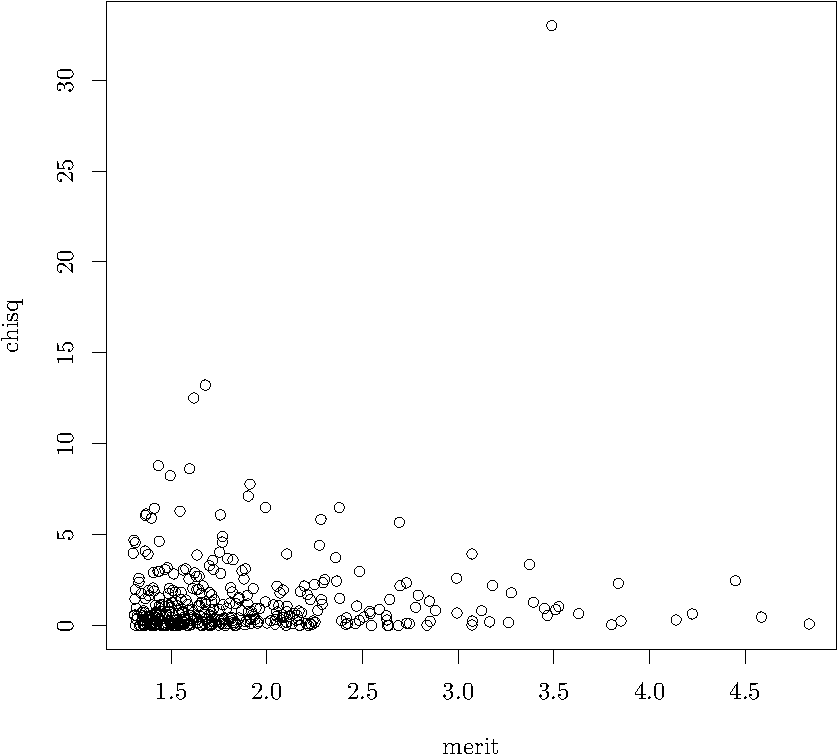
\includegraphics[width=\maxwidth]{figure/07-E3-E3-val-1} 

}


\begin{kframe}\begin{alltt}
\hlkwd{plot}\hlstd{(chisq} \hlopt{~} \hlstd{merit, val.TCGA.messina)}
\end{alltt}
\end{kframe}

{\centering 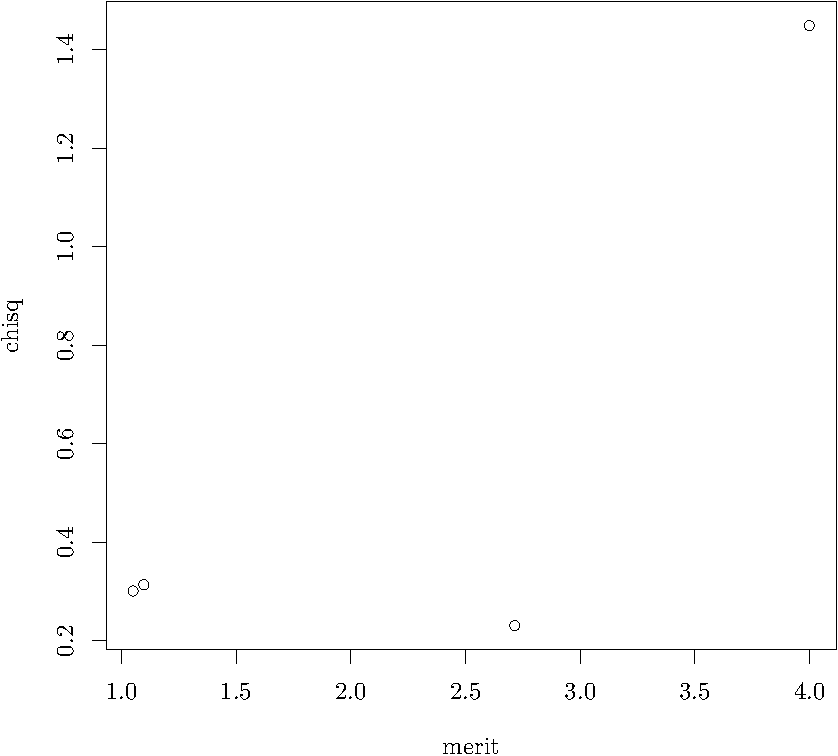
\includegraphics[width=\maxwidth]{figure/07-E3-E3-val-2} 

}


\begin{kframe}\begin{alltt}
\hlkwd{plot}\hlstd{(chisq} \hlopt{~} \hlstd{merit, val.comb.maxstat)}
\end{alltt}
\end{kframe}

{\centering 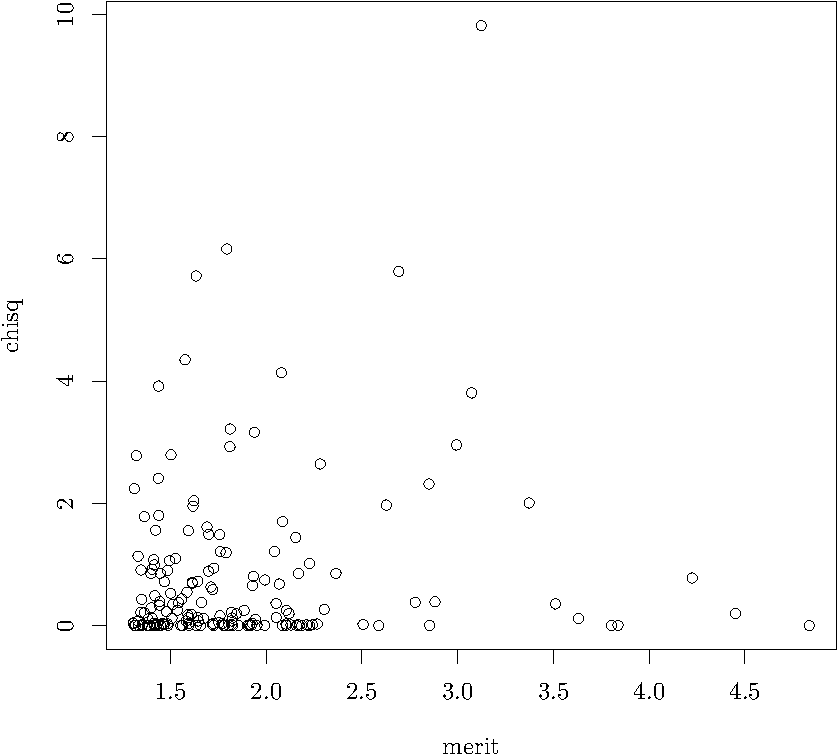
\includegraphics[width=\maxwidth]{figure/07-E3-E3-val-3} 

}


\begin{kframe}\begin{alltt}
\hlkwd{plot}\hlstd{(chisq} \hlopt{~} \hlstd{merit, val.comb.messina)}
\end{alltt}
\end{kframe}

{\centering 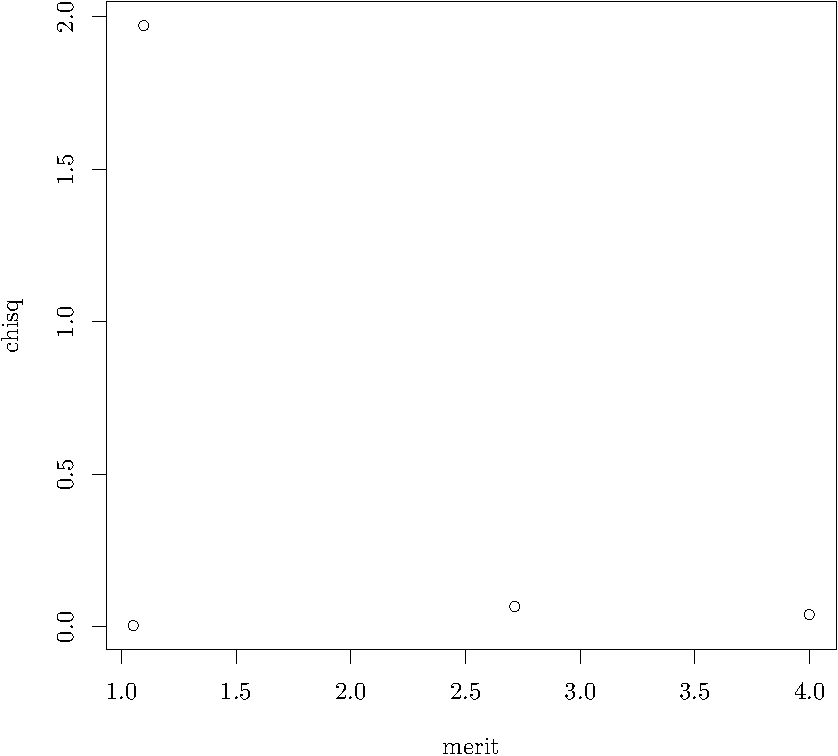
\includegraphics[width=\maxwidth]{figure/07-E3-E3-val-4} 

}



\end{knitrout}


\begin{knitrout}
\definecolor{shadecolor}{rgb}{0.969, 0.969, 0.969}\color{fgcolor}\begin{kframe}
\begin{alltt}
\hlkwd{library}\hlstd{(messina)}
\hlkwd{library}\hlstd{(ggplot2)}
\hlkwd{library}\hlstd{(grid)}
\hlcom{# library(doMC)}
\hlcom{# registerDoMC(4)}
\hlcom{# temp.fit.messina = messinaSurv(APGI.x[c("KRT6A", "ANGPTL4", "KRT6C"),], APGI.y, messinaSurvObj.CoxCoef(round(log(2), 3)), parallel = FALSE, silent = FALSE, seed = 20150321)}
\hlkwd{print}\hlstd{(APGI.messina)}
\end{alltt}
\begin{verbatim}
## An object of class MessinaSurvResult
## 
## Problem type:survival
## Parameters:
##   An object of class MessinaParameters
##   13000 features, 110 samples.
##   Objective type: survival [messinaSurvObj.CoxCoef(coxcoef_threshold = 0.693)].
##   Minimum group fraction: 0.1
##   Training fraction: 0.8
##   Number of bootstraps: 50
##   Random seed: 20150321
## 
## Summary of results:
##   An object of class MessinaFits
##   159 / 13000 features passed performance requirements (1.22%)
##   Top features:
##         Passed Requirements Classifier Type Threshold Value Direction
## KRT6A                  TRUE       Threshold           9.503         1
## ANGPTL4                TRUE       Threshold           8.900         1
## KRT6C                  TRUE       Threshold           7.458         1
## IGFBP1                 TRUE       Threshold           7.070         1
## FGG                    TRUE       Threshold           8.585         1
## LYNX1                  TRUE       Threshold           7.020         1
## PPY                    TRUE       Threshold          11.931        -1
## LOX                    TRUE       Threshold           7.686         1
## DCBLD2                 TRUE       Threshold          10.959         1
## CDA                    TRUE       Threshold           8.205         1
##         Margin
## KRT6A   3.9988
## ANGPTL4 2.7155
## KRT6C   2.3334
## IGFBP1  1.4736
## FGG     1.3648
## LYNX1   1.3442
## PPY     1.0981
## LOX     1.0514
## DCBLD2  0.9851
## CDA     0.9712
\end{verbatim}
\begin{alltt}
\hlkwd{pdf}\hlstd{(}\hlstr{"07_E3_best.pdf"}\hlstd{,} \hlkwc{height} \hlstd{=} \hlnum{8}\hlstd{,} \hlkwc{width} \hlstd{=} \hlnum{6}\hlstd{)}
\hlkwd{plot}\hlstd{(APGI.messina,} \hlkwc{indices} \hlstd{=} \hlnum{1}\hlopt{:}\hlnum{3}\hlstd{)}
\end{alltt}


{\ttfamily\noindent\color{warningcolor}{\#\# Warning: Removed 2 rows containing missing values (geom\_path).}}

{\ttfamily\noindent\color{warningcolor}{\#\# Warning: Removed 2 rows containing missing values (geom\_path).}}

{\ttfamily\noindent\color{warningcolor}{\#\# Warning: Removed 2 rows containing missing values (geom\_path).}}\begin{alltt}
\hlcom{# plot(APGI.messina, indices = 1:3, bootstrap_type = "ci")}

\hlkwd{pushViewport}\hlstd{(}\hlkwd{viewport}\hlstd{(}\hlkwc{layout} \hlstd{=} \hlkwd{grid.layout}\hlstd{(}\hlnum{3}\hlstd{,} \hlnum{2}\hlstd{)))}

\hlstd{i} \hlkwb{=} \hlkwd{which}\hlstd{(}\hlkwd{rownames}\hlstd{(APGI.messina}\hlopt{@}\hlkwc{fits}\hlopt{@}\hlkwc{summary}\hlstd{)} \hlopt{==} \hlstr{"KRT6A"}\hlstd{)}
\hlstd{plt1} \hlkwb{=} \hlstd{messina}\hlopt{:::}\hlkwd{messinaSurvObjPlot}\hlstd{(APGI.messina, i)} \hlopt{+} \hlkwd{geom_rug}\hlstd{(}\hlkwd{aes}\hlstd{(}\hlkwc{x} \hlstd{= x),} \hlkwc{data} \hlstd{=} \hlkwd{data.frame}\hlstd{(}\hlkwc{x} \hlstd{= APGI.x[}\hlstr{"KRT6A"}\hlstd{,],} \hlkwc{Objective} \hlstd{=} \hlnum{0}\hlstd{,} \hlkwc{Alpha} \hlstd{=} \hlnum{0.25}\hlstd{),} \hlkwc{sides} \hlstd{=} \hlstr{"b"}\hlstd{,} \hlkwc{size} \hlstd{=} \hlnum{1.5}\hlstd{)} \hlopt{+} \hlkwd{theme_bw}\hlstd{()} \hlopt{+} \hlkwd{theme}\hlstd{(}\hlkwc{legend.position} \hlstd{=} \hlstr{"none"}\hlstd{)}
\hlstd{plt2} \hlkwb{=} \hlstd{messina}\hlopt{:::}\hlkwd{messinaSurvKMplot}\hlstd{(}\hlkwc{y} \hlstd{=} \hlkwd{Surv}\hlstd{(APGI.y[,}\hlnum{1}\hlstd{]}\hlopt{/}\hlnum{365.25}\hlopt{*}\hlnum{12}\hlstd{, APGI.y[,}\hlnum{2}\hlstd{]),} \hlkwc{group} \hlstd{= (APGI.x[}\hlstr{"KRT6A"}\hlstd{,]} \hlopt{>} \hlstd{APGI.messina}\hlopt{@}\hlkwc{fits}\hlopt{@}\hlkwc{summary}\hlopt{$}\hlstd{threshold[i])}\hlopt{*}\hlnum{1}\hlstd{,} \hlkwc{bootstrap_type} \hlstd{=} \hlstr{"ci"}\hlstd{,} \hlkwc{bootstrap_ci} \hlstd{=} \hlnum{0.9}\hlstd{,} \hlkwc{nboot} \hlstd{=} \hlnum{500}\hlstd{,} \hlkwc{parallel} \hlstd{=} \hlnum{FALSE}\hlstd{)} \hlopt{+} \hlkwd{theme_bw}\hlstd{()} \hlopt{+} \hlkwd{theme}\hlstd{(}\hlkwc{legend.position} \hlstd{=} \hlstr{"none"}\hlstd{)}
\hlkwd{print}\hlstd{(plt1,} \hlkwc{vp} \hlstd{=} \hlkwd{viewport}\hlstd{(}\hlkwc{layout.pos.row} \hlstd{=} \hlnum{1}\hlstd{,} \hlkwc{layout.pos.col} \hlstd{=} \hlnum{1}\hlstd{))}
\end{alltt}


{\ttfamily\noindent\color{warningcolor}{\#\# Warning: Removed 2 rows containing missing values (geom\_path).}}\begin{alltt}
\hlkwd{print}\hlstd{(plt2,} \hlkwc{vp} \hlstd{=} \hlkwd{viewport}\hlstd{(}\hlkwc{layout.pos.row} \hlstd{=} \hlnum{1}\hlstd{,} \hlkwc{layout.pos.col} \hlstd{=} \hlnum{2}\hlstd{))}

\hlcom{# print(messina:::messinaSurvKMplot(y = APGI.y, group = (APGI.x["KRT6A",] > APGI.messina@fits@summary$threshold[i] - APGI.messina@fits@summary$margin[i]/2)*1, bootstrap_type = "ci", bootstrap_ci = 0.9, nboot = 500, parallel = FALSE) + ggtitle("Separation at Lower Boundary") + theme(legend.position = "bottom"))}
\hlcom{# print(messina:::messinaSurvKMplot(y = APGI.y, group = (APGI.x["KRT6A",] > APGI.messina@fits@summary$threshold[i] + APGI.messina@fits@summary$margin[i]/2)*1, bootstrap_type = "ci", bootstrap_ci = 0.9, nboot = 500, parallel = FALSE) + ggtitle("Separation at Upper Boundary") + theme(legend.position = "bottom"))}

\hlstd{i} \hlkwb{=} \hlkwd{which}\hlstd{(}\hlkwd{rownames}\hlstd{(APGI.messina}\hlopt{@}\hlkwc{fits}\hlopt{@}\hlkwc{summary}\hlstd{)} \hlopt{==} \hlstr{"ANGPTL4"}\hlstd{)}
\hlstd{plt1} \hlkwb{=} \hlstd{messina}\hlopt{:::}\hlkwd{messinaSurvObjPlot}\hlstd{(APGI.messina, i)} \hlopt{+} \hlkwd{geom_rug}\hlstd{(}\hlkwd{aes}\hlstd{(}\hlkwc{x} \hlstd{= x),} \hlkwc{data} \hlstd{=} \hlkwd{data.frame}\hlstd{(}\hlkwc{x} \hlstd{= APGI.x[}\hlstr{"ANGPTL4"}\hlstd{,],} \hlkwc{Objective} \hlstd{=} \hlnum{0}\hlstd{,} \hlkwc{Alpha} \hlstd{=} \hlnum{0.25}\hlstd{),} \hlkwc{sides} \hlstd{=} \hlstr{"b"}\hlstd{,} \hlkwc{size} \hlstd{=} \hlnum{1.5}\hlstd{)} \hlopt{+} \hlkwd{theme_bw}\hlstd{()} \hlopt{+} \hlkwd{theme}\hlstd{(}\hlkwc{legend.position} \hlstd{=} \hlstr{"none"}\hlstd{)}
\hlstd{plt2} \hlkwb{=} \hlstd{messina}\hlopt{:::}\hlkwd{messinaSurvKMplot}\hlstd{(}\hlkwc{y} \hlstd{=} \hlkwd{Surv}\hlstd{(APGI.y[,}\hlnum{1}\hlstd{]}\hlopt{/}\hlnum{365.25}\hlopt{*}\hlnum{12}\hlstd{, APGI.y[,}\hlnum{2}\hlstd{]),} \hlkwc{group} \hlstd{= (APGI.x[}\hlstr{"ANGPTL4"}\hlstd{,]} \hlopt{>} \hlstd{APGI.messina}\hlopt{@}\hlkwc{fits}\hlopt{@}\hlkwc{summary}\hlopt{$}\hlstd{threshold[i])}\hlopt{*}\hlnum{1}\hlstd{,} \hlkwc{bootstrap_type} \hlstd{=} \hlstr{"ci"}\hlstd{,} \hlkwc{bootstrap_ci} \hlstd{=} \hlnum{0.9}\hlstd{,} \hlkwc{nboot} \hlstd{=} \hlnum{500}\hlstd{,} \hlkwc{parallel} \hlstd{=} \hlnum{FALSE}\hlstd{)} \hlopt{+} \hlkwd{theme_bw}\hlstd{()} \hlopt{+} \hlkwd{theme}\hlstd{(}\hlkwc{legend.position} \hlstd{=} \hlstr{"none"}\hlstd{)}
\hlkwd{print}\hlstd{(plt1,} \hlkwc{vp} \hlstd{=} \hlkwd{viewport}\hlstd{(}\hlkwc{layout.pos.row} \hlstd{=} \hlnum{2}\hlstd{,} \hlkwc{layout.pos.col} \hlstd{=} \hlnum{1}\hlstd{))}
\end{alltt}


{\ttfamily\noindent\color{warningcolor}{\#\# Warning: Removed 2 rows containing missing values (geom\_path).}}\begin{alltt}
\hlkwd{print}\hlstd{(plt2,} \hlkwc{vp} \hlstd{=} \hlkwd{viewport}\hlstd{(}\hlkwc{layout.pos.row} \hlstd{=} \hlnum{2}\hlstd{,} \hlkwc{layout.pos.col} \hlstd{=} \hlnum{2}\hlstd{))}
\hlcom{# print(messina:::messinaSurvKMplot(y = APGI.y, group = (APGI.x["ANGPTL4",] > APGI.messina@fits@summary$threshold[i] - APGI.messina@fits@summary$margin[i]/2)*1, bootstrap_type = "ci", bootstrap_ci = 0.9, nboot = 500, parallel = FALSE) + ggtitle("Separation at Lower Boundary") + theme(legend.position = "bottom"))}
\hlcom{# print(messina:::messinaSurvKMplot(y = APGI.y, group = (APGI.x["ANGPTL4",] > APGI.messina@fits@summary$threshold[i] + APGI.messina@fits@summary$margin[i]/2)*1, bootstrap_type = "ci", bootstrap_ci = 0.9, nboot = 500, parallel = FALSE) + ggtitle("Separation at Upper Boundary") + theme(legend.position = "bottom"))}

\hlstd{i} \hlkwb{=} \hlkwd{which}\hlstd{(}\hlkwd{rownames}\hlstd{(APGI.messina}\hlopt{@}\hlkwc{fits}\hlopt{@}\hlkwc{summary}\hlstd{)} \hlopt{==} \hlstr{"KRT6C"}\hlstd{)}
\hlstd{plt1} \hlkwb{=} \hlstd{messina}\hlopt{:::}\hlkwd{messinaSurvObjPlot}\hlstd{(APGI.messina, i)} \hlopt{+} \hlkwd{geom_rug}\hlstd{(}\hlkwd{aes}\hlstd{(}\hlkwc{x} \hlstd{= x),} \hlkwc{data} \hlstd{=} \hlkwd{data.frame}\hlstd{(}\hlkwc{x} \hlstd{= APGI.x[}\hlstr{"KRT6C"}\hlstd{,],} \hlkwc{Objective} \hlstd{=} \hlnum{0}\hlstd{,} \hlkwc{Alpha} \hlstd{=} \hlnum{0.25}\hlstd{),} \hlkwc{sides} \hlstd{=} \hlstr{"b"}\hlstd{,} \hlkwc{size} \hlstd{=} \hlnum{1.5}\hlstd{)} \hlopt{+} \hlkwd{theme_bw}\hlstd{()} \hlopt{+} \hlkwd{theme}\hlstd{(}\hlkwc{legend.position} \hlstd{=} \hlstr{"none"}\hlstd{)}
\hlstd{plt2} \hlkwb{=} \hlstd{messina}\hlopt{:::}\hlkwd{messinaSurvKMplot}\hlstd{(}\hlkwc{y} \hlstd{=} \hlkwd{Surv}\hlstd{(APGI.y[,}\hlnum{1}\hlstd{]}\hlopt{/}\hlnum{365.25}\hlopt{*}\hlnum{12}\hlstd{, APGI.y[,}\hlnum{2}\hlstd{]),} \hlkwc{group} \hlstd{= (APGI.x[}\hlstr{"KRT6C"}\hlstd{,]} \hlopt{>} \hlstd{APGI.messina}\hlopt{@}\hlkwc{fits}\hlopt{@}\hlkwc{summary}\hlopt{$}\hlstd{threshold[i])}\hlopt{*}\hlnum{1}\hlstd{,} \hlkwc{bootstrap_type} \hlstd{=} \hlstr{"ci"}\hlstd{,} \hlkwc{bootstrap_ci} \hlstd{=} \hlnum{0.9}\hlstd{,} \hlkwc{nboot} \hlstd{=} \hlnum{500}\hlstd{,} \hlkwc{parallel} \hlstd{=} \hlnum{FALSE}\hlstd{)} \hlopt{+} \hlkwd{theme_bw}\hlstd{()} \hlopt{+} \hlkwd{theme}\hlstd{(}\hlkwc{legend.position} \hlstd{=} \hlstr{"none"}\hlstd{)}
\hlkwd{print}\hlstd{(plt1,} \hlkwc{vp} \hlstd{=} \hlkwd{viewport}\hlstd{(}\hlkwc{layout.pos.row} \hlstd{=} \hlnum{3}\hlstd{,} \hlkwc{layout.pos.col} \hlstd{=} \hlnum{1}\hlstd{))}
\end{alltt}


{\ttfamily\noindent\color{warningcolor}{\#\# Warning: Removed 2 rows containing missing values (geom\_path).}}\begin{alltt}
\hlkwd{print}\hlstd{(plt2,} \hlkwc{vp} \hlstd{=} \hlkwd{viewport}\hlstd{(}\hlkwc{layout.pos.row} \hlstd{=} \hlnum{3}\hlstd{,} \hlkwc{layout.pos.col} \hlstd{=} \hlnum{2}\hlstd{))}
\hlcom{# print(messina:::messinaSurvKMplot(y = APGI.y, group = (APGI.x["KRT6C",] > APGI.messina@fits@summary$threshold[i] - APGI.messina@fits@summary$margin[i]/2)*1, bootstrap_type = "ci", bootstrap_ci = 0.9, nboot = 500, parallel = FALSE) + ggtitle("Separation at Lower Boundary") + theme(legend.position = "bottom"))}
\hlcom{# print(messina:::messinaSurvKMplot(y = APGI.y, group = (APGI.x["KRT6C",] > APGI.messina@fits@summary$threshold[i] + APGI.messina@fits@summary$margin[i]/2)*1, bootstrap_type = "ci", bootstrap_ci = 0.9, nboot = 500, parallel = FALSE) + ggtitle("Separation at Upper Boundary") + theme(legend.position = "bottom"))}

\hlkwd{dev.off}\hlstd{()}
\end{alltt}
\begin{verbatim}
## pdf 
##   2
\end{verbatim}
\end{kframe}
\end{knitrout}


\begin{knitrout}
\definecolor{shadecolor}{rgb}{0.969, 0.969, 0.969}\color{fgcolor}\begin{kframe}
\begin{alltt}
\hlstd{val.GSE28735.messina} \hlkwb{=} \hlkwd{doValidation}\hlstd{(}\hlkwd{as.character}\hlstd{(APGI.feats}\hlopt{$}\hlstd{symbol), APGI.x, APGI.messina}\hlopt{@}\hlkwc{fits}\hlopt{@}\hlkwc{summary}\hlopt{$}\hlstd{threshold, APGI.messina}\hlopt{@}\hlkwc{fits}\hlopt{@}\hlkwc{summary}\hlopt{$}\hlstd{margin} \hlopt{*} \hlstd{APGI.messina}\hlopt{@}\hlkwc{fits}\hlopt{@}\hlkwc{summary}\hlopt{$}\hlstd{passed,} \hlnum{0}\hlstd{,} \hlkwd{as.character}\hlstd{(GSE28735.feats}\hlopt{$}\hlstd{Gene.symbol), GSE28735.x, GSE28735.y)}
\hlstd{val.GSE28735.maxstat} \hlkwb{=} \hlkwd{doValidation}\hlstd{(}\hlkwd{as.character}\hlstd{(APGI.feats}\hlopt{$}\hlstd{symbol), APGI.x,} \hlkwd{sapply}\hlstd{(APGI.maxstat,} \hlkwa{function}\hlstd{(}\hlkwc{x}\hlstd{) x}\hlopt{$}\hlstd{threshold),} \hlopt{-}\hlkwd{log10}\hlstd{(}\hlkwd{sapply}\hlstd{(APGI.maxstat,} \hlkwa{function}\hlstd{(}\hlkwc{x}\hlstd{) x}\hlopt{$}\hlstd{p.value)),} \hlnum{0}\hlstd{,} \hlkwd{as.character}\hlstd{(GSE28735.feats}\hlopt{$}\hlstd{Gene.symbol), GSE28735.x, GSE28735.y)}
\hlstd{val.GSE21501.messina} \hlkwb{=} \hlkwd{doValidation}\hlstd{(}\hlkwd{as.character}\hlstd{(APGI.feats}\hlopt{$}\hlstd{symbol), APGI.x, APGI.messina}\hlopt{@}\hlkwc{fits}\hlopt{@}\hlkwc{summary}\hlopt{$}\hlstd{threshold, APGI.messina}\hlopt{@}\hlkwc{fits}\hlopt{@}\hlkwc{summary}\hlopt{$}\hlstd{margin} \hlopt{*} \hlstd{APGI.messina}\hlopt{@}\hlkwc{fits}\hlopt{@}\hlkwc{summary}\hlopt{$}\hlstd{passed,} \hlnum{0}\hlstd{,} \hlkwd{as.character}\hlstd{(GSE21501.feats}\hlopt{$}\hlstd{Gene.symbol), GSE21501.x, GSE21501.y)}
\hlstd{val.GSE21501.maxstat} \hlkwb{=} \hlkwd{doValidation}\hlstd{(}\hlkwd{as.character}\hlstd{(APGI.feats}\hlopt{$}\hlstd{symbol), APGI.x,} \hlkwd{sapply}\hlstd{(APGI.maxstat,} \hlkwa{function}\hlstd{(}\hlkwc{x}\hlstd{) x}\hlopt{$}\hlstd{threshold),} \hlopt{-}\hlkwd{log10}\hlstd{(}\hlkwd{sapply}\hlstd{(APGI.maxstat,} \hlkwa{function}\hlstd{(}\hlkwc{x}\hlstd{) x}\hlopt{$}\hlstd{p.value)),} \hlnum{0}\hlstd{,} \hlkwd{as.character}\hlstd{(GSE21501.feats}\hlopt{$}\hlstd{Gene.symbol), GSE21501.x, GSE21501.y)}
\hlstd{val.TCGA.messina} \hlkwb{=} \hlkwd{doValidation}\hlstd{(}\hlkwd{as.character}\hlstd{(APGI.feats}\hlopt{$}\hlstd{symbol), APGI.x, APGI.messina}\hlopt{@}\hlkwc{fits}\hlopt{@}\hlkwc{summary}\hlopt{$}\hlstd{threshold, APGI.messina}\hlopt{@}\hlkwc{fits}\hlopt{@}\hlkwc{summary}\hlopt{$}\hlstd{margin} \hlopt{*} \hlstd{APGI.messina}\hlopt{@}\hlkwc{fits}\hlopt{@}\hlkwc{summary}\hlopt{$}\hlstd{passed,} \hlnum{0}\hlstd{,} \hlkwd{as.character}\hlstd{(TCGA.feats}\hlopt{$}\hlstd{symbol), TCGA.x, TCGA.y)}
\hlstd{val.TCGA.maxstat} \hlkwb{=} \hlkwd{doValidation}\hlstd{(}\hlkwd{as.character}\hlstd{(APGI.feats}\hlopt{$}\hlstd{symbol), APGI.x,} \hlkwd{sapply}\hlstd{(APGI.maxstat,} \hlkwa{function}\hlstd{(}\hlkwc{x}\hlstd{) x}\hlopt{$}\hlstd{threshold),} \hlopt{-}\hlkwd{log10}\hlstd{(}\hlkwd{sapply}\hlstd{(APGI.maxstat,} \hlkwa{function}\hlstd{(}\hlkwc{x}\hlstd{) x}\hlopt{$}\hlstd{p.value)),} \hlnum{0}\hlstd{,} \hlkwd{as.character}\hlstd{(TCGA.feats}\hlopt{$}\hlstd{symbol), TCGA.x, TCGA.y)}
\hlstd{val.comb.messina} \hlkwb{=} \hlkwd{doValidation}\hlstd{(}\hlkwd{as.character}\hlstd{(APGI.feats}\hlopt{$}\hlstd{symbol), APGI.x, APGI.messina}\hlopt{@}\hlkwc{fits}\hlopt{@}\hlkwc{summary}\hlopt{$}\hlstd{threshold, APGI.messina}\hlopt{@}\hlkwc{fits}\hlopt{@}\hlkwc{summary}\hlopt{$}\hlstd{margin} \hlopt{*} \hlstd{APGI.messina}\hlopt{@}\hlkwc{fits}\hlopt{@}\hlkwc{summary}\hlopt{$}\hlstd{passed,} \hlnum{0}\hlstd{,} \hlkwd{as.character}\hlstd{(comb.feats}\hlopt{$}\hlstd{symbol), comb.x, comb.y)}
\hlstd{val.comb.maxstat} \hlkwb{=} \hlkwd{doValidation}\hlstd{(}\hlkwd{as.character}\hlstd{(APGI.feats}\hlopt{$}\hlstd{symbol), APGI.x,} \hlkwd{sapply}\hlstd{(APGI.maxstat,} \hlkwa{function}\hlstd{(}\hlkwc{x}\hlstd{) x}\hlopt{$}\hlstd{threshold),} \hlopt{-}\hlkwd{log10}\hlstd{(}\hlkwd{sapply}\hlstd{(APGI.maxstat,} \hlkwa{function}\hlstd{(}\hlkwc{x}\hlstd{) x}\hlopt{$}\hlstd{p.value)),} \hlnum{0}\hlstd{,} \hlkwd{as.character}\hlstd{(comb.feats}\hlopt{$}\hlstd{symbol), comb.x, comb.y)}
\hlstd{val.GSE28735.messina2} \hlkwb{=} \hlkwd{doValidation}\hlstd{(}\hlkwd{as.character}\hlstd{(APGI.feats}\hlopt{$}\hlstd{symbol), APGI.x, APGI.messina}\hlopt{@}\hlkwc{fits}\hlopt{@}\hlkwc{summary}\hlopt{$}\hlstd{threshold, APGI.messina}\hlopt{@}\hlkwc{fits}\hlopt{@}\hlkwc{summary}\hlopt{$}\hlstd{margin,} \hlnum{0}\hlstd{,} \hlkwd{as.character}\hlstd{(GSE28735.feats}\hlopt{$}\hlstd{Gene.symbol), GSE28735.x, GSE28735.y)}
\hlstd{val.GSE21501.messina2} \hlkwb{=} \hlkwd{doValidation}\hlstd{(}\hlkwd{as.character}\hlstd{(APGI.feats}\hlopt{$}\hlstd{symbol), APGI.x, APGI.messina}\hlopt{@}\hlkwc{fits}\hlopt{@}\hlkwc{summary}\hlopt{$}\hlstd{threshold, APGI.messina}\hlopt{@}\hlkwc{fits}\hlopt{@}\hlkwc{summary}\hlopt{$}\hlstd{margin,} \hlnum{0}\hlstd{,} \hlkwd{as.character}\hlstd{(GSE21501.feats}\hlopt{$}\hlstd{Gene.symbol), GSE21501.x, GSE21501.y)}
\hlstd{val.TCGA.messina2} \hlkwb{=} \hlkwd{doValidation}\hlstd{(}\hlkwd{as.character}\hlstd{(APGI.feats}\hlopt{$}\hlstd{symbol), APGI.x, APGI.messina}\hlopt{@}\hlkwc{fits}\hlopt{@}\hlkwc{summary}\hlopt{$}\hlstd{threshold, APGI.messina}\hlopt{@}\hlkwc{fits}\hlopt{@}\hlkwc{summary}\hlopt{$}\hlstd{margin,} \hlnum{0}\hlstd{,} \hlkwd{as.character}\hlstd{(TCGA.feats}\hlopt{$}\hlstd{symbol), TCGA.x, TCGA.y)}
\hlstd{val.comb.messina2} \hlkwb{=} \hlkwd{doValidation}\hlstd{(}\hlkwd{as.character}\hlstd{(APGI.feats}\hlopt{$}\hlstd{symbol), APGI.x, APGI.messina}\hlopt{@}\hlkwc{fits}\hlopt{@}\hlkwc{summary}\hlopt{$}\hlstd{threshold, APGI.messina}\hlopt{@}\hlkwc{fits}\hlopt{@}\hlkwc{summary}\hlopt{$}\hlstd{margin,} \hlnum{0}\hlstd{,} \hlkwd{as.character}\hlstd{(comb.feats}\hlopt{$}\hlstd{symbol), comb.x, comb.y)}

\hlkwd{print}\hlstd{(val.GSE28735.messina[val.GSE28735.messina}\hlopt{$}\hlstd{merit} \hlopt{>=} \hlnum{1}\hlstd{,])}
\end{alltt}
\begin{verbatim}
##         merit threshold.train threshold.test  chisq abs.hr
## KRT6A   3.999           9.503          4.754 1.6382 0.4753
## ANGPTL4 2.716           8.900          3.754 0.6709 0.3042
## FGG     1.365           8.585         13.796     NA     NA
## PPY     1.098          11.931          4.068 2.5368 0.5915
## LOX     1.051           7.686          6.841 0.4943 0.2611
\end{verbatim}
\begin{alltt}
\hlkwd{print}\hlstd{(val.GSE21501.messina[val.GSE21501.messina}\hlopt{$}\hlstd{merit} \hlopt{>=} \hlnum{1}\hlstd{,])}
\end{alltt}
\begin{verbatim}
##         merit threshold.train threshold.test  chisq  abs.hr
## KRT6A   3.999           9.503         3.3849 0.2333 0.11891
## ANGPTL4 2.716           8.900         0.7529 0.1246 0.08691
## KRT6C   2.333           7.458        40.3387     NA      NA
## IGFBP1  1.474           7.070        -4.0458 2.3645 0.37856
## FGG     1.365           8.585         9.7976     NA      NA
## PPY     1.098          11.931         3.8380 0.3419 0.14395
## LOX     1.051           7.686        -0.5062 0.1867 0.10636
\end{verbatim}
\begin{alltt}
\hlkwd{print}\hlstd{(val.TCGA.messina[val.TCGA.messina}\hlopt{$}\hlstd{merit} \hlopt{>=} \hlnum{1}\hlstd{,])}
\end{alltt}
\begin{verbatim}
##         merit threshold.train threshold.test  chisq abs.hr
## KRT6A   3.999           9.503          3.656 1.4483 0.5838
## ANGPTL4 2.716           8.900          3.336 0.2310 0.2331
## KRT6C   2.333           7.458         16.773     NA     NA
## IGFBP1  1.474           7.070          3.788     NA     NA
## FGG     1.365           8.585         10.219     NA     NA
## LYNX1   1.344           7.020          3.998     NA     NA
## PPY     1.098          11.931          3.969 0.3139 0.2718
## LOX     1.051           7.686          3.602 0.3011 0.2662
\end{verbatim}
\begin{alltt}
\hlkwd{print}\hlstd{(val.comb.messina[val.comb.messina}\hlopt{$}\hlstd{merit} \hlopt{>=} \hlnum{1}\hlstd{,])}
\end{alltt}
\begin{verbatim}
##         merit threshold.train threshold.test    chisq  abs.hr
## KRT6A   3.999           9.503          4.029 0.039744 0.05879
## ANGPTL4 2.716           8.900          3.359 0.066278 0.07592
## FGG     1.365           8.585         12.497       NA      NA
## PPY     1.098          11.931          4.015 1.971306 0.41403
## LOX     1.051           7.686          3.810 0.003568 0.01761
\end{verbatim}
\begin{alltt}
\hlkwd{print}\hlstd{(val.GSE28735.messina2[val.GSE28735.messina2}\hlopt{$}\hlstd{merit} \hlopt{>=} \hlnum{1}\hlstd{,])}
\end{alltt}
\begin{verbatim}
##         merit threshold.train threshold.test    chisq  abs.hr
## KRT6A   3.999           9.503          4.754 1.638186 0.47535
## ANGPTL4 2.716           8.900          3.754 0.670894 0.30420
## DHRS9   1.468           8.965          4.404 0.007037 0.03116
## FGG     1.365           8.585         13.796       NA      NA
## PPY     1.098          11.931          4.068 2.536840 0.59153
## LOX     1.051           7.686          6.841 0.494314 0.26112
## IL20RB  1.043           6.971          4.060 0.435502 0.24509
\end{verbatim}
\begin{alltt}
\hlkwd{print}\hlstd{(val.GSE21501.messina2[val.GSE21501.messina2}\hlopt{$}\hlstd{merit} \hlopt{>=} \hlnum{1}\hlstd{,])}
\end{alltt}
\begin{verbatim}
##         merit threshold.train threshold.test  chisq  abs.hr
## KRT6A   3.999           9.503         3.3849 0.2333 0.11891
## ANGPTL4 2.716           8.900         0.7529 0.1246 0.08691
## KRT6C   2.333           7.458        40.3387     NA      NA
## IGFBP1  1.474           7.070        -4.0458 2.3645 0.37856
## DHRS9   1.468           8.965         1.9614 3.9596 0.48988
## FGG     1.365           8.585         9.7976     NA      NA
## PPY     1.098          11.931         3.8380 0.3419 0.14395
## LOX     1.051           7.686        -0.5062 0.1867 0.10636
## IL20RB  1.043           6.971         1.7140 0.6682 0.20124
\end{verbatim}
\begin{alltt}
\hlkwd{print}\hlstd{(val.TCGA.messina2[val.TCGA.messina2}\hlopt{$}\hlstd{merit} \hlopt{>=} \hlnum{1}\hlstd{,])}
\end{alltt}
\begin{verbatim}
##         merit threshold.train threshold.test  chisq abs.hr
## KRT6A   3.999           9.503          3.656 1.4483 0.5838
## ANGPTL4 2.716           8.900          3.336 0.2310 0.2331
## KRT6C   2.333           7.458         16.773     NA     NA
## CIDEC   2.269           8.021          3.192 2.0245 0.6902
## IGFBP1  1.474           7.070          3.788     NA     NA
## DHRS9   1.468           8.965          3.203 0.1557 0.1914
## FGG     1.365           8.585         10.219     NA     NA
## LYNX1   1.344           7.020          3.998     NA     NA
## PPY     1.098          11.931          3.969 0.3139 0.2718
## LOX     1.051           7.686          3.602 0.3011 0.2662
## IL20RB  1.043           6.971          2.975 4.0928 0.9813
\end{verbatim}
\begin{alltt}
\hlkwd{print}\hlstd{(val.comb.messina2[val.comb.messina2}\hlopt{$}\hlstd{merit} \hlopt{>=} \hlnum{1}\hlstd{,])}
\end{alltt}
\begin{verbatim}
##         merit threshold.train threshold.test    chisq  abs.hr
## KRT6A   3.999           9.503          4.029 0.039744 0.05879
## ANGPTL4 2.716           8.900          3.359 0.066278 0.07592
## DHRS9   1.468           8.965          3.237 0.023762 0.04546
## FGG     1.365           8.585         12.497       NA      NA
## PPY     1.098          11.931          4.015 1.971306 0.41403
## LOX     1.051           7.686          3.810 0.003568 0.01761
## IL20RB  1.043           6.971          3.407 1.555023 0.36772
\end{verbatim}
\begin{alltt}
\hlkwd{print}\hlstd{(val.GSE28735.messina2[}\hlnum{1}\hlopt{:}\hlnum{25}\hlstd{,])}
\end{alltt}
\begin{verbatim}
##           merit threshold.train threshold.test    chisq  abs.hr
## KRT6A    3.9988           9.503          4.754 1.638186 0.47535
## ANGPTL4  2.7155           8.900          3.754 0.670894 0.30420
## DHRS9    1.4685           8.965          4.404 0.007037 0.03116
## FGG      1.3648           8.585         13.796       NA      NA
## PPY      1.0981          11.931          4.068 2.536840 0.59153
## LOX      1.0514           7.686          6.841 0.494314 0.26112
## IL20RB   1.0429           6.971          4.060 0.435502 0.24509
## DCBLD2   0.9851          10.959          8.809 4.573332 0.79423
## CDA      0.9712           8.205          5.484 5.578617 0.87719
## PYGL     0.9394           8.707          6.968 1.675156 0.48068
## TCEA3    0.8598           9.056          4.960 6.722756 0.96295
## DKK1     0.7932          10.123          5.601 4.468957 0.78512
## SERPINB3 0.7304           7.502          8.703 0.434203 0.24472
## CAV1     0.7152          10.833          6.383 1.861383 0.50670
## UBE2C    0.7069           9.361          5.275 1.842838 0.50417
## UPP1     0.6954           9.363          4.612 2.009762 0.52651
## COL17A1  0.6772          10.850          6.112 0.916987 0.35564
## NEK2     0.6470           8.382          4.655 3.762606 0.72040
## TGFBI    0.6440          11.519          7.745 1.997784 0.52493
## PHLDA1   0.6227           9.838          6.666 1.301754 0.42374
## CDC20    0.6035           9.036          4.516 1.048897 0.38036
## FGB      0.5720           6.942          4.373 0.482299 0.25792
## SPOCK1   0.5481           8.806          5.282 5.432086 0.86559
## KLHL5    0.5450           9.040          6.523 1.858889 0.50636
## KCTD10   0.5421           8.313          6.391 0.954290 0.36280
\end{verbatim}
\begin{alltt}
\hlkwd{print}\hlstd{(val.GSE21501.messina2[}\hlnum{1}\hlopt{:}\hlnum{25}\hlstd{,])}
\end{alltt}
\begin{verbatim}
##           merit threshold.train threshold.test   chisq  abs.hr
## KRT6A    3.9988           9.503         3.3849  0.2333 0.11891
## ANGPTL4  2.7155           8.900         0.7529  0.1246 0.08691
## KRT6C    2.3334           7.458        40.3387      NA      NA
## IGFBP1   1.4736           7.070        -4.0458  2.3645 0.37856
## DHRS9    1.4685           8.965         1.9614  3.9596 0.48988
## FGG      1.3648           8.585         9.7976      NA      NA
## PPY      1.0981          11.931         3.8380  0.3419 0.14395
## LOX      1.0514           7.686        -0.5062  0.1867 0.10636
## IL20RB   1.0429           6.971         1.7140  0.6682 0.20124
## DCBLD2   0.9851          10.959         0.8818  5.1370 0.55797
## TCEA3    0.8598           9.056         0.8150  3.8451 0.48274
## DKK1     0.7932          10.123         1.0495  1.5160 0.30311
## SERPINB3 0.7304           7.502         9.8687      NA      NA
## CAV1     0.7152          10.833        -0.4123  0.3670 0.14913
## UBE2C    0.7069           9.361        -1.0727  2.2779 0.37156
## COL17A1  0.6772          10.850         4.3181  0.1625 0.09925
## NEK2     0.6470           8.382        -1.4027  1.7177 0.32265
## TGFBI    0.6440          11.519         0.4992  0.1565 0.09738
## FGB      0.5720           6.942         4.3258  1.5532 0.30681
## PHACTR3  0.5493           6.744         1.8219  1.4980 0.30131
## SPOCK1   0.5481           8.806        -0.2239  0.1803 0.10452
## F3       0.5411           9.489         3.6157  2.2244 0.36717
## TMEM158  0.5410          10.672         2.4477  0.7650 0.21532
## ADM      0.4839           8.850        -1.6351  3.8843 0.48519
## ERRFI1   0.4786          10.269         0.6604 16.4916 0.99975
\end{verbatim}
\begin{alltt}
\hlkwd{print}\hlstd{(val.TCGA.messina2[}\hlnum{1}\hlopt{:}\hlnum{25}\hlstd{,])}
\end{alltt}
\begin{verbatim}
##           merit threshold.train threshold.test  chisq  abs.hr
## KRT6A    3.9988           9.503          3.656 1.4483 0.58375
## ANGPTL4  2.7155           8.900          3.336 0.2310 0.23314
## KRT6C    2.3334           7.458         16.773     NA      NA
## CIDEC    2.2689           8.021          3.192 2.0245 0.69018
## IGFBP1   1.4736           7.070          3.788     NA      NA
## DHRS9    1.4685           8.965          3.203 0.1557 0.19137
## FGG      1.3648           8.585         10.219     NA      NA
## LYNX1    1.3442           7.020          3.998     NA      NA
## PPY      1.0981          11.931          3.969 0.3139 0.27177
## LOX      1.0514           7.686          3.602 0.3011 0.26619
## IL20RB   1.0429           6.971          2.975 4.0928 0.98133
## DCBLD2   0.9851          10.959          3.702 0.4372 0.32074
## CDA      0.9712           8.205          3.461 1.6185 0.61711
## PYGL     0.9394           8.707          3.452 3.7715 0.94202
## TCEA3    0.8598           9.056          3.289 1.6718 0.62719
## DKK1     0.7932          10.123          3.661     NA      NA
## SERPINB3 0.7304           7.502          6.685     NA      NA
## CAV1     0.7152          10.833          3.700 0.7929 0.43194
## UBE2C    0.7069           9.361          3.293 4.1776 0.99145
## UPP1     0.6954           9.363          3.369 0.0271 0.07985
## COL17A1  0.6772          10.850          3.644 3.8883 0.95650
## NEK2     0.6470           8.382          3.223 2.0679 0.69754
## TGFBI    0.6440          11.519          3.793 9.1433 1.46676
## PHLDA1   0.6227           9.838          3.699 0.2173 0.22611
## CDC20    0.6035           9.036          3.264 1.0556 0.49836
\end{verbatim}
\begin{alltt}
\hlkwd{print}\hlstd{(val.comb.messina2[}\hlnum{1}\hlopt{:}\hlnum{25}\hlstd{,])}
\end{alltt}
\begin{verbatim}
##           merit threshold.train threshold.test    chisq  abs.hr
## KRT6A    3.9988           9.503          4.029 0.039744 0.05879
## ANGPTL4  2.7155           8.900          3.359 0.066278 0.07592
## DHRS9    1.4685           8.965          3.237 0.023762 0.04546
## FGG      1.3648           8.585         12.497       NA      NA
## PPY      1.0981          11.931          4.015 1.971306 0.41403
## LOX      1.0514           7.686          3.810 0.003568 0.01761
## IL20RB   1.0429           6.971          3.407 1.555023 0.36772
## DCBLD2   0.9851          10.959          4.201 0.003568 0.01761
## CDA      0.9712           8.205          4.503 0.042036 0.06046
## PYGL     0.9394           8.707          3.652 0.003568 0.01761
## TCEA3    0.8598           9.056          2.882       NA      NA
## DKK1     0.7932          10.123          4.422 1.830767 0.39900
## SERPINB3 0.7304           7.502          7.088 0.062874 0.07394
## CAV1     0.7152          10.833          4.066 0.003568 0.01761
## UBE2C    0.7069           9.361          3.757 0.038753 0.05805
## UPP1     0.6954           9.363          3.623 0.133938 0.10792
## COL17A1  0.6772          10.850          3.799 1.218751 0.32554
## NEK2     0.6470           8.382          3.602 1.057385 0.30323
## TGFBI    0.6440          11.519          3.851 1.315357 0.33820
## PHLDA1   0.6227           9.838          3.846 0.003568 0.01761
## CDC20    0.6035           9.036          3.671 0.076721 0.08168
## FGB      0.5720           6.942          4.752 0.140356 0.11048
## SPOCK1   0.5481           8.806          3.649 0.242147 0.14511
## KLHL5    0.5450           9.040          3.478 1.047763 0.30184
## KCTD10   0.5421           8.313          3.652 0.003568 0.01761
\end{verbatim}
\begin{alltt}
\hlkwd{print}\hlstd{(val.GSE28735.maxstat[val.GSE28735.maxstat}\hlopt{$}\hlstd{merit} \hlopt{>= -}\hlkwd{log10}\hlstd{(}\hlnum{0.01}\hlstd{),])}
\end{alltt}
\begin{verbatim}
##          merit threshold.train threshold.test     chisq  abs.hr
## ANGPTL4  4.835           8.356          3.527 1.2172131 0.40975
## KRT6A    4.450           8.915          4.503 2.1797169 0.54832
## LOX      4.225           7.502          6.609 0.5418944 0.27339
## PYGL     3.837           8.829          7.074 2.2505118 0.55715
## ST6GAL1  3.803           9.542          6.145 1.2301143 0.41191
## FAM189A2 3.630           6.455          4.052 0.0031968 0.02100
## KLHL5    3.511           8.978          6.464 2.7284225 0.61346
## ADM      3.394           8.820          4.730 1.0881259 0.38741
## E2F7     3.373           6.507          3.854 4.9383591 0.82532
## SMOX     3.165           7.190          4.852 0.0264970 0.06045
## KIF20A   3.123           7.250          3.584 2.3964258 0.57493
## CAPN6    3.073           6.516          4.094 0.7537046 0.32243
## IL20RB   2.994           6.505          3.492 0.6900670 0.30852
## P4HA1    2.882           9.080          7.426 0.0361759 0.07064
## FYN      2.854           8.079          6.086 0.5063749 0.26428
## AURKA    2.850           7.727          3.628 0.5199047 0.26779
## TCEA3    2.791           8.955          4.898 3.5465208 0.69941
## LOXL4    2.778           7.628          3.985 0.0043526 0.02450
## LDHA     2.744          11.922          9.716 0.6055617 0.28901
## CKAP2L   2.693           7.047          3.898 3.2384237 0.66834
## PPY      2.628          11.966          4.074 2.5368403 0.59153
## TREM1    2.588           6.546          5.146 0.3641295 0.22411
## PLOD1    2.541          10.492          5.802 0.0607022 0.09150
## CDC20    2.506           8.806          4.385 0.7903335 0.33017
## PFKP     2.483           9.183          5.636 0.0770144 0.10307
## ERRFI1   2.364          10.222          8.463 0.0265727 0.06054
## RGS5     2.303           8.665          6.941 0.1157263 0.12634
## TPX2     2.283           7.213          4.613 2.3417950 0.56834
## P4HA2    2.267           9.209          6.579 2.3446584 0.56868
## SLC15A1  2.242           6.716          5.053 0.4827903 0.25805
## DPY19L1  2.227           9.183          6.364 0.0340304 0.06851
## MME      2.227           6.441          4.645 0.1424883 0.14019
## ATF7IP2  2.212           7.139          5.793 0.0462345 0.07986
## PAEP     2.186           6.304          5.022 0.2213571 0.17473
## EPHX2    2.173           7.223          3.637 0.7331425 0.31800
## KYNU     2.169           7.161          5.370 0.0009540 0.01147
## FOXM1    2.166           6.884          4.573 5.9976088 0.90954
## NAMPT    2.159           7.988         10.049 0.3699184 0.22588
## PLOD2    2.155          10.451          7.593 3.3000992 0.67467
## UPP1     2.130           9.094          4.411 1.2476835 0.41484
## KCTD10   2.119           7.907          6.094 0.0003352 0.00680
## ZNF185   2.105           7.420          3.933 1.0598714 0.38235
## EDIL3    2.105           6.400          8.217 0.0054087 0.02731
## NEK2     2.103           8.167          4.426 0.5031598 0.26344
## LCP1     2.100           8.702          6.629 6.4127584 0.94049
## GAPDH    2.086          11.336          9.814 1.9514902 0.51882
## ARSD     2.085           9.970          6.440 2.8660524 0.62874
## KIF2C    2.080           6.839          3.953 3.6289488 0.70749
## ENO2     2.069           7.557          5.422 0.0374754 0.07190
## COL12A1  2.052           8.689          8.314 0.0572269 0.08884
## VSNL1    2.052           6.712          4.221 0.0023373 0.01796
## ENTHD1   2.044           6.345          3.130 0.1850704 0.15977
## CADPS2   2.043           7.892          5.795 3.0258048 0.64603
\end{verbatim}
\begin{alltt}
\hlkwd{print}\hlstd{(val.GSE21501.maxstat[val.GSE21501.maxstat}\hlopt{$}\hlstd{merit} \hlopt{>= -}\hlkwd{log10}\hlstd{(}\hlnum{0.01}\hlstd{),])}
\end{alltt}
\begin{verbatim}
##          merit threshold.train threshold.test    chisq  abs.hr
## ANGPTL4  4.835           8.356        0.19587  0.68647 0.20397
## KRT6A    4.450           8.915        2.97484  0.02615 0.03981
## LOX      4.225           7.502       -0.79221  1.05819 0.25324
## KRT6C    4.215           6.392        5.59238       NA      NA
## ST6GAL1  3.803           9.542        0.78319  0.57393 0.18650
## FAM189A2 3.630           6.455        0.28808  0.72477 0.20958
## ADM      3.394           8.820       -1.66023  7.68147 0.68231
## E2F7     3.373           6.507       -2.26972 11.01337 0.81699
## CAPN6    3.073           6.516        0.58777  1.93415 0.34238
## IL20RB   2.994           6.505        0.27819  2.88983 0.41850
## FGF13    2.837           6.400       -0.33980  2.19688 0.36489
## TCEA3    2.791           8.955        0.67789  4.56051 0.52573
## LOXL4    2.778           7.628        0.96728  0.44986 0.16512
## TMEM26   2.688           6.692        0.77037  0.04695 0.05334
## BIRC5    2.643           7.334       -1.61111  4.02097 0.49365
## CD70     2.632           6.748       -0.60306  0.50354 0.17469
## PPY      2.628          11.966        3.85564  0.78045 0.21749
## TREM1    2.588           6.546        2.12235  4.16653 0.50251
## IGFBP1   2.466           7.076       -4.02812  1.67463 0.31858
## ERRFI1   2.364          10.222        0.59119 17.90323 1.04165
## RGS5     2.303           8.665        4.26999  5.36891 0.57043
## PHACTR3  2.275           6.884        1.98393  1.34315 0.28531
## MME      2.227           6.441       -1.58576  0.21888 0.11518
## PRDM16   2.206           6.605        3.97296  1.83929 0.33387
## PAEP     2.186           6.304        0.77117  0.42416 0.16033
## EPHX2    2.173           7.223        0.03016  0.45635 0.16631
## KYNU     2.169           7.161       -1.99673  0.37952 0.15166
## NAMPT    2.159           7.988        0.11528  1.97005 0.34554
## PLOD2    2.155          10.451        0.06961  0.08655 0.07243
## EDIL3    2.105           6.400        4.24471  1.30442 0.28117
## NEK2     2.103           8.167       -1.80395  4.75048 0.53657
## LCP1     2.100           8.702       -1.84614  2.89631 0.41897
## COL12A1  2.052           8.689        1.83301  0.30533 0.13603
## VSNL1    2.052           6.712       -1.64740  0.15289 0.09626
## ENTHD1   2.044           6.345        1.75682  0.26324 0.12631
## PCDH20   2.003           7.551        3.99419  1.35435 0.28650
\end{verbatim}
\begin{alltt}
\hlkwd{print}\hlstd{(val.TCGA.maxstat[val.TCGA.maxstat}\hlopt{$}\hlstd{merit} \hlopt{>= -}\hlkwd{log10}\hlstd{(}\hlnum{0.01}\hlstd{),])}
\end{alltt}
\begin{verbatim}
##          merit threshold.train threshold.test     chisq   abs.hr
## ANGPTL4  4.835           8.356         3.2506 8.573e-02 0.142030
## B3GALTL  4.586           6.747         3.1744 4.692e-01 0.332277
## KRT6A    4.450           8.915         3.5365 2.464e+00 0.761458
## LOX      4.225           7.502         3.5709 6.397e-01 0.387968
## KRT6C    4.215           6.392         3.9993        NA       NA
## PFKFB4   4.140           7.004         3.0053 3.090e-01 0.269623
## CIDEC    3.851           7.623         3.0437 2.472e-01 0.241173
## PYGL     3.837           8.829         3.4693 2.323e+00 0.739303
## ST6GAL1  3.803           9.542         3.6540 4.597e-02 0.104006
## FAM189A2 3.630           6.455         2.8347 6.560e-01 0.392865
## RPIA     3.527           7.988         3.2886 1.041e+00 0.494966
## KLHL5    3.511           8.978         3.4314 8.833e-01 0.455900
## LYNX1    3.490           6.603         3.5629 3.300e+01 2.786522
## TRAPPC2  3.466           8.229         3.2071 5.559e-01 0.361659
## ZNF565   3.451           6.532         2.8439 9.433e-01 0.471122
## ADM      3.394           8.820         3.0578 1.290e+00 0.550837
## E2F7     3.373           6.507         2.8931 3.369e+00 0.890337
## KTI12    3.278           7.949         3.1614 1.803e+00 0.651319
## UFC1     3.264           9.787         3.5679 1.613e-01 0.194826
## HJURP    3.180           6.967         3.1594 2.203e+00 0.719982
## SMOX     3.165           7.190         3.2938 2.054e-01 0.219816
## KIF20A   3.123           7.250         3.1635 8.137e-01 0.437564
## ELMOD3   3.075           7.298         3.2690 2.506e-01 0.242803
## NACC2    3.073           6.578         2.7790 3.077e-02 0.085091
## CAPN6    3.073           6.516         3.1289 3.945e+00 0.963493
## IL20RB   2.994           6.505         2.6696 6.952e-01 0.404444
## CARHSP1  2.993          10.451         3.5607 2.610e+00 0.783592
## P4HA1    2.882           9.080         3.5537 8.216e-01 0.439679
## FYN      2.854           8.079         3.5020 2.393e-01 0.237278
## AURKA    2.850           7.727         3.1350 1.347e+00 0.562947
## FGF13    2.837           6.400         2.8910 2.202e-02 0.071977
## TCEA3    2.791           8.955         3.2703 1.672e+00 0.627186
## LOXL4    2.778           7.628         3.2741 1.007e+00 0.486752
## LDHA     2.744          11.922         3.8200 1.032e-01 0.155810
## SLAMF9   2.730           6.346         1.9189 2.350e+00 0.743553
## GOLPH3L  2.729           7.859         3.4711 1.324e-01 0.176470
## DEFB123  2.716           6.326            NaN        NA       NA
## SLC30A3  2.696           6.399         1.5633 2.190e+00 0.717762
## CKAP2L   2.693           7.047         3.0517 5.679e+00 1.155938
## TMEM26   2.688           6.692         2.8280 5.494e-05 0.003595
## BIRC5    2.643           7.334         3.1152 1.436e+00 0.581364
## IFT140   2.638           6.438         3.3541 3.296e-03 0.027850
## CD70     2.632           6.748         2.6457 3.625e-03 0.029205
## PPY      2.628          11.966         3.9751 3.139e-01 0.271774
## LRRFIP2  2.624           7.861         3.4000 5.492e-01 0.359463
## TREM1    2.588           6.546         3.0622 8.990e-01 0.459927
## LYRM1    2.548           9.343         3.2709 5.861e-03 0.037136
## PLOD1    2.541          10.492         3.6442 6.590e-01 0.393765
## ATP5O    2.538          11.228         3.6003 7.877e-01 0.430499
## CDC20    2.506           8.806         3.2186 4.668e-01 0.331426
## ARHGEF19 2.486           6.695         3.1074 2.975e+00 0.836710
## PFKP     2.483           9.183         3.5533 2.849e-01 0.258895
## AURKB    2.470           6.963         3.0300 1.073e+00 0.502561
## IGFBP1   2.466           7.076         3.7990        NA       NA
## VPS29    2.464           9.524         3.3949 1.012e-01 0.154339
## PHF21A   2.423           8.261         3.3828 1.254e-01 0.171748
## PDCD2L   2.416           7.446         2.9782 4.223e-01 0.315233
## FAH      2.413           7.260         3.2812 6.847e-02 0.126932
## PLIN3    2.391          11.237         3.6267 2.658e-01 0.250069
## SLC15A4  2.382           9.055         3.4043 1.492e+00 0.592598
## NOTCH1   2.378           7.822         3.4138 6.490e+00 1.235773
## ERRFI1   2.364          10.222         3.7131 2.452e+00 0.759630
## RFX4     2.360           6.318         0.6094 3.735e+00 0.937419
## RGS5     2.303           8.665         3.6868 2.529e+00 0.771462
## COL5A3   2.294           6.444         3.3676 2.353e+00 0.744144
## PTPRM    2.289           7.564         3.4899 1.177e+00 0.526291
## SOBP     2.285           7.318         3.2145 1.427e+00 0.579445
## TPX2     2.283           7.213         3.4056 5.839e+00 1.172127
## PHACTR3  2.275           6.884         2.7109 4.422e+00 1.020010
## P4HA2    2.267           9.209         3.5563 8.348e-01 0.443197
## IKBIP    2.252           6.947         3.3099 1.815e-01 0.206659
## DHRS11   2.249           7.620         3.0378 2.263e+00 0.729748
## SLC15A1  2.242           6.716         3.2639 2.503e-01 0.242659
## BMS1     2.234           9.010         3.4895 4.549e-02 0.103453
## DPY19L1  2.227           9.183         3.5265 1.193e-01 0.167516
## MME      2.227           6.441         3.1336 1.430e+00 0.580049
## ARMC7    2.218           7.589         3.2933 1.957e-03 0.021460
## ATF7IP2  2.212           7.139         3.2603 1.696e+00 0.631663
## PRDM16   2.206           6.605         3.2494 1.055e-01 0.157519
## TRIM54   2.197           8.060         3.1774 2.177e+00 0.715766
## PAEP     2.186           6.304         3.5895        NA       NA
## TM9SF3   2.181           9.973         3.8034 7.033e-01 0.406800
## TARBP2   2.175           6.959         3.2777 1.864e+00 0.662262
## EPHX2    2.173           7.223         3.1924 1.516e-04 0.005973
## SGSM1    2.171           6.631         2.9490 2.006e-02 0.068698
## KYNU     2.169           7.161         3.1598 8.082e-01 0.436070
## FOXM1    2.166           6.884         3.3186 3.181e-01 0.273580
## NAMPT    2.159           7.988         3.6866 5.716e-01 0.366727
## PLOD2    2.155          10.451         3.5670 2.931e-01 0.262627
## TTC13    2.144           7.827         3.3152 6.849e-01 0.401449
## UPP1     2.130           9.094         3.3237 9.579e-02 0.150132
## KCTD10   2.119           7.907         3.5420 5.250e-01 0.351483
## ZNF185   2.105           7.420         3.2864 1.071e+00 0.502018
## EDIL3    2.105           6.400         3.5273 3.943e+00 0.963201
## KCNQ3    2.104           6.635         2.5387 7.679e-01 0.425055
## NEK2     2.103           8.167         3.1637 1.973e-01 0.215456
## LCP1     2.100           8.702         3.5387 9.984e-03 0.048469
## CFL1     2.088          12.385         3.9427 4.260e-01 0.316604
## GAPDH    2.086          11.336         4.0228 1.957e+00 0.678555
## ARSD     2.085           9.970         3.6909 5.880e-01 0.371959
## PGBD3    2.085           6.454         2.9488 1.496e-01 0.187636
## KIF2C    2.080           6.839         3.2058 4.434e-01 0.322993
## ENO2     2.069           7.557         3.4295 1.791e+00 0.649226
## ABLIM1   2.063           9.734         3.6850 1.090e+00 0.506472
## RFC5     2.053           7.876         3.1563 2.165e+00 0.713759
## COL12A1  2.052           8.689         3.7775 5.110e-01 0.346739
## VSNL1    2.052           6.712         2.9368 7.472e-01 0.419295
## ENTHD1   2.044           6.345         2.9963 3.341e-01 0.280367
## CADPS2   2.043           7.892         3.3495 7.356e-02 0.131561
## GARS     2.035          10.140         3.5755 1.141e+00 0.518191
## SCYL2    2.021           8.564         3.4991 2.646e-01 0.249525
## PCDH20   2.003           7.551         3.5025        NA       NA
## ARFGAP3  2.001           8.794         3.5346 1.388e-01 0.180722
\end{verbatim}
\begin{alltt}
\hlkwd{print}\hlstd{(val.comb.maxstat[val.comb.maxstat}\hlopt{$}\hlstd{merit} \hlopt{>= -}\hlkwd{log10}\hlstd{(}\hlnum{0.01}\hlstd{),])}
\end{alltt}
\begin{verbatim}
##          merit threshold.train threshold.test     chisq   abs.hr
## ANGPTL4  4.835           8.356          3.210 0.0004978 0.006579
## KRT6A    4.450           8.915          3.844 0.1986036 0.131415
## LOX      4.225           7.502          3.674 0.7779826 0.260097
## PYGL     3.837           8.829          3.749 0.0035678 0.017614
## ST6GAL1  3.803           9.542          3.897 0.0035678 0.017614
## FAM189A2 3.630           6.455          3.141 0.1145970 0.099825
## KLHL5    3.511           8.978          3.436 0.3554151 0.175800
## ADM      3.394           8.820          2.480        NA       NA
## E2F7     3.373           6.507          3.226 2.0068826 0.417746
## SMOX     3.165           7.190          3.061        NA       NA
## KIF20A   3.123           7.250          3.215 9.8111520 0.923658
## CAPN6    3.073           6.516          3.026 3.8052088 0.575228
## IL20RB   2.994           6.505          2.897 2.9543186 0.506850
## P4HA1    2.882           9.080          3.664 0.3896693 0.184077
## FYN      2.854           8.079          3.627 0.0035678 0.017614
## AURKA    2.850           7.727          3.251 2.3172761 0.448890
## TCEA3    2.791           8.955          2.794        NA       NA
## LOXL4    2.778           7.628          3.277 0.3821183 0.182285
## LDHA     2.744          11.922          3.593        NA       NA
## CKAP2L   2.693           7.047          3.391 5.7916593 0.709664
## PPY      2.628          11.966          4.021 1.9713060 0.414026
## TREM1    2.588           6.546          3.178 0.0007441 0.008044
## PLOD1    2.541          10.492          3.522        NA       NA
## CDC20    2.506           8.806          3.501 0.0187455 0.040374
## PFKP     2.483           9.183          3.236        NA       NA
## ERRFI1   2.364          10.222          3.697 0.8531713 0.272376
## RGS5     2.303           8.665          3.744 0.2652384 0.151869
## TPX2     2.283           7.213          3.573 2.6441369 0.479505
## P4HA2    2.267           9.209          3.663 0.0253982 0.046995
## SLC15A1  2.242           6.716          3.477 0.0144333 0.035427
## DPY19L1  2.227           9.183          3.721 0.0035678 0.017614
## MME      2.227           6.441          3.198 1.0129642 0.296789
## ATF7IP2  2.212           7.139          3.843 0.0117813 0.032007
## PAEP     2.186           6.304          6.323 0.0004239 0.006071
## EPHX2    2.173           7.223          3.219 0.0086576 0.027438
## KYNU     2.169           7.161          2.993 0.8499361 0.271859
## FOXM1    2.166           6.884          3.573 0.0187455 0.040374
## NAMPT    2.159           7.988          3.765 0.0055932 0.022054
## PLOD2    2.155          10.451          3.540 1.4408075 0.353960
## UPP1     2.130           9.094          3.431 0.0119443 0.032228
## KCTD10   2.119           7.907          3.504 0.1981721 0.131272
## ZNF185   2.105           7.420          2.953 0.2493545 0.147251
## EDIL3    2.105           6.400          4.043 0.0035678 0.017614
## NEK2     2.103           8.167          3.437 0.0269672 0.048425
## LCP1     2.100           8.702          3.003        NA       NA
## GAPDH    2.086          11.336          4.025 1.6997840 0.384457
## ARSD     2.085           9.970          4.143 0.0035678 0.017614
## KIF2C    2.080           6.839          3.346 4.1336140 0.599537
## ENO2     2.069           7.557          3.319 0.6803431 0.243229
## COL12A1  2.052           8.689          3.651 0.1334730 0.107733
## VSNL1    2.052           6.712          3.189 0.3629304 0.177649
## ENTHD1   2.044           6.345          3.456 1.2111259 0.324523
## CADPS2   2.043           7.892          3.059        NA       NA
\end{verbatim}
\begin{alltt}
\hlcom{# detCurve(list(}
\hlcom{# 	"Messina GSE28735" = val.GSE28735.messina, }
\hlcom{# 	"Messina GSE21501" = val.GSE21501.messina, }
\hlcom{# 	"Messina TCGA" = val.TCGA.messina, }
\hlcom{# 	"Messina GSE28735 NC" = val.GSE28735.messina2, }
\hlcom{# 	"Messina GSE21501 NC" = val.GSE21501.messina2, }
\hlcom{# 	"Messina TCGA NC" = val.TCGA.messina2, }
\hlcom{# 	"maxstat GSE28735" = val.GSE28735.maxstat, }
\hlcom{# 	"maxstat GSE21501" = val.GSE21501.maxstat, }
\hlcom{# 	"maxstat TCGA" = val.TCGA.maxstat)) + theme_bw()}
\end{alltt}
\end{kframe}
\end{knitrout}

\begin{knitrout}
\definecolor{shadecolor}{rgb}{0.969, 0.969, 0.969}\color{fgcolor}\begin{kframe}
\begin{alltt}
\hlstd{detCurve} \hlkwb{=} \hlkwa{function}\hlstd{(}\hlkwc{val_list}\hlstd{,} \hlkwc{alpha} \hlstd{=} \hlnum{0.05}\hlstd{,} \hlkwc{relative} \hlstd{=} \hlnum{FALSE}\hlstd{,} \hlkwc{dataonly} \hlstd{=} \hlnum{FALSE}\hlstd{)}
\hlstd{\{}
        \hlkwa{if} \hlstd{(}\hlkwd{is.null}\hlstd{(}\hlkwd{names}\hlstd{(val_list)))}
        \hlstd{\{}
                \hlkwd{names}\hlstd{(val_list)} \hlkwb{=} \hlkwd{paste}\hlstd{(}\hlstr{"Method"}\hlstd{,} \hlnum{1}\hlopt{:}\hlkwd{length}\hlstd{(val_list),} \hlkwc{sep} \hlstd{=} \hlstr{" "}\hlstd{)}
        \hlstd{\}}

        \hlstd{val_list_annotated} \hlkwb{=} \hlkwd{lapply}\hlstd{(val_list,} \hlkwa{function}\hlstd{(}\hlkwc{val}\hlstd{) \{}
                \hlstd{val}\hlopt{$}\hlstd{merit[}\hlkwd{is.na}\hlstd{(val}\hlopt{$}\hlstd{merit)]} \hlkwb{=} \hlopt{-}\hlnum{1}
                \hlstd{val} \hlkwb{=} \hlstd{val[}\hlkwd{order}\hlstd{(}\hlopt{-}\hlstd{val}\hlopt{$}\hlstd{merit),]}
                \hlstd{val}\hlopt{$}\hlstd{val} \hlkwb{=} \hlkwd{pchisq}\hlstd{(val}\hlopt{$}\hlstd{chisq,} \hlkwc{df} \hlstd{=} \hlnum{1}\hlstd{,} \hlkwc{lower.tail} \hlstd{=} \hlnum{FALSE}\hlstd{)} \hlopt{<} \hlstd{alpha}
                \hlstd{val}\hlopt{$}\hlstd{val[}\hlkwd{is.na}\hlstd{(val}\hlopt{$}\hlstd{chisq)]} \hlkwb{=} \hlnum{FALSE}
                \hlstd{val}\hlopt{$}\hlstd{cum_val} \hlkwb{=} \hlkwd{cumsum}\hlstd{(val}\hlopt{$}\hlstd{val)}
                \hlstd{val}\hlopt{$}\hlstd{cum_nonval} \hlkwb{=} \hlkwd{cumsum}\hlstd{(}\hlopt{!}\hlstd{val}\hlopt{$}\hlstd{val)}
                \hlstd{total_val} \hlkwb{=} \hlkwd{sum}\hlstd{(val}\hlopt{$}\hlstd{val)}
                \hlstd{total_nonval} \hlkwb{=} \hlkwd{sum}\hlstd{(}\hlopt{!}\hlstd{val}\hlopt{$}\hlstd{val)}
                \hlstd{val}\hlopt{$}\hlstd{rate_val} \hlkwb{=} \hlstd{val}\hlopt{$}\hlstd{cum_val} \hlopt{/} \hlstd{total_val}
                \hlstd{val}\hlopt{$}\hlstd{rate_nonval} \hlkwb{=} \hlstd{val}\hlopt{$}\hlstd{cum_nonval} \hlopt{/} \hlstd{total_nonval}
                \hlstd{val}
        \hlstd{\})}

        \hlstd{val_list_combined} \hlkwb{=} \hlkwd{do.call}\hlstd{(rbind, val_list_annotated)}
        \hlstd{val_list_combined}\hlopt{$}\hlstd{Curve} \hlkwb{=} \hlkwd{rep}\hlstd{(}\hlkwd{names}\hlstd{(val_list),} \hlkwd{sapply}\hlstd{(val_list, nrow))}

        \hlkwa{if} \hlstd{(dataonly)   \{} \hlkwd{return}\hlstd{(val_list_combined) \}}
        \hlkwa{if} \hlstd{(}\hlopt{!}\hlstd{relative)}
        \hlstd{\{}
                \hlstd{nval} \hlkwb{=} \hlkwd{sapply}\hlstd{(val_list_annotated,} \hlkwa{function}\hlstd{(}\hlkwc{v}\hlstd{)} \hlkwd{sum}\hlstd{(v}\hlopt{$}\hlstd{val))}
                \hlstd{null_slopes} \hlkwb{=} \hlkwd{data.frame}\hlstd{(}\hlkwc{Curve} \hlstd{=} \hlkwd{names}\hlstd{(nval),} \hlkwc{intercept} \hlstd{=} \hlnum{0}\hlstd{,} \hlkwc{slope} \hlstd{= nval)}

                \hlstd{theplot} \hlkwb{=} \hlkwd{ggplot}\hlstd{(val_list_combined,} \hlkwd{aes}\hlstd{(}\hlkwc{x} \hlstd{= rate_nonval,} \hlkwc{y} \hlstd{= cum_val,} \hlkwc{colour} \hlstd{= Curve))} \hlopt{+}
                        \hlkwd{geom_line}\hlstd{(}\hlkwc{lwd} \hlstd{=} \hlnum{2}\hlstd{)} \hlopt{+}
                        \hlkwd{xlab}\hlstd{(}\hlstr{"Non-validation rate"}\hlstd{)} \hlopt{+}
                        \hlkwd{ylab}\hlstd{(}\hlstr{"Total validated"}\hlstd{)} \hlopt{+}
                        \hlkwd{geom_abline}\hlstd{(}\hlkwd{aes}\hlstd{(}\hlkwc{intercept} \hlstd{= intercept,} \hlkwc{slope} \hlstd{= slope,} \hlkwc{colour} \hlstd{= Curve), null_slopes,} \hlkwc{linetype} \hlstd{=} \hlstr{"dashed"}\hlstd{,} \hlkwc{lwd} \hlstd{=} \hlnum{1.5}\hlstd{)}
        \hlstd{\}}
        \hlkwa{else}
        \hlstd{\{}
                \hlstd{theplot} \hlkwb{=} \hlkwd{ggplot}\hlstd{(val_list_combined,} \hlkwd{aes}\hlstd{(}\hlkwc{x} \hlstd{= rate_nonval,} \hlkwc{y} \hlstd{= rate_val,} \hlkwc{colour} \hlstd{= Curve))} \hlopt{+}
                        \hlkwd{geom_line}\hlstd{(}\hlkwc{lwd} \hlstd{=} \hlnum{2}\hlstd{)} \hlopt{+}
                        \hlkwd{xlab}\hlstd{(}\hlstr{"Non-validation rate"}\hlstd{)} \hlopt{+}
                        \hlkwd{ylab}\hlstd{(}\hlstr{"Validation rate"}\hlstd{)} \hlopt{+}
                        \hlkwd{geom_abline}\hlstd{(}\hlkwc{intercept} \hlstd{=} \hlnum{0}\hlstd{,} \hlkwc{slope} \hlstd{=} \hlnum{1}\hlstd{,} \hlkwc{linetype} \hlstd{=} \hlstr{"dashed"}\hlstd{,} \hlkwc{lwd} \hlstd{=} \hlnum{1.5}\hlstd{)} \hlopt{+}
                        \hlkwd{xlim}\hlstd{(}\hlnum{0}\hlstd{,} \hlnum{1}\hlstd{)} \hlopt{+} \hlkwd{ylim}\hlstd{(}\hlnum{0}\hlstd{,} \hlnum{1}\hlstd{)}
        \hlstd{\}}

        \hlstd{theplot}
\hlstd{\}}

\hlcom{# detCurve(list(Messina = val.GSE28735.messina, maxstat = val.GSE28735.maxstat, MessinaCore = val.GSE28735.messina2)) + theme_bw() + xlim(0, 0.2) + ylim(0, 70) + theme(legend.position = "none")}
\hlcom{# detCurve(list(Messina = val.GSE28735.messina, maxstat = val.GSE28735.maxstat, MessinaCore = val.GSE28735.messina2), relative = TRUE) + theme_bw() + theme(legend.position = "none")}
\hlcom{# detCurve(list(Messina = val.GSE21501.messina, maxstat = val.GSE21501.maxstat, MessinaCore = val.GSE21501.messina2)) + theme_bw() + xlim(0, 0.2) + ylim(0, 60) + theme(legend.position = "none")}
\hlcom{# detCurve(list(Messina = val.GSE21501.messina, maxstat = val.GSE21501.maxstat, MessinaCore = val.GSE21501.messina2), relative = TRUE) + theme_bw() + theme(legend.position = "none")}
\hlcom{# detCurve(list(Messina = val.TCGA.messina, maxstat = val.TCGA.maxstat, MessinaCore = val.TCGA.messina2)) + theme_bw() + xlim(0, 0.2) + ylim(0, 200) + labs(colour = "Method") + theme(legend.position = "none")}
\hlcom{# detCurve(list(Messina = val.TCGA.messina, maxstat = val.TCGA.maxstat, MessinaCore = val.TCGA.messina2), relative = TRUE) + theme_bw() + labs(colour = "Method") + theme(legend.position = "none")}
\hlcom{# detCurve(list(Messina = val.comb.messina, maxstat = val.comb.maxstat, MessinaCore = val.comb.messina2)) + theme_bw() + xlim(0, 0.2) + ylim(0, 200) + labs(colour = "Method") + theme(legend.position = "none")}
\hlcom{# detCurve(list(Messina = val.comb.messina, maxstat = val.comb.maxstat, MessinaCore = val.comb.messina2), relative = TRUE) + theme_bw() + labs(colour = "Method") + theme(legend.position = "none")}

\hlstd{dat1} \hlkwb{=} \hlkwd{detCurve}\hlstd{(}\hlkwd{list}\hlstd{(}\hlkwc{Messina} \hlstd{= val.GSE28735.messina,} \hlkwc{maxstat} \hlstd{= val.GSE28735.maxstat,} \hlkwc{Messina2Core} \hlstd{= val.GSE28735.messina2),} \hlkwc{dataonly} \hlstd{=} \hlnum{TRUE}\hlstd{)}
\hlstd{dat2} \hlkwb{=} \hlkwd{detCurve}\hlstd{(}\hlkwd{list}\hlstd{(}\hlkwc{Messina} \hlstd{= val.TCGA.messina,} \hlkwc{maxstat} \hlstd{= val.TCGA.maxstat,} \hlkwc{Messina2Core} \hlstd{= val.TCGA.messina2),} \hlkwc{dataonly} \hlstd{=} \hlnum{TRUE}\hlstd{)}
\hlstd{data} \hlkwb{=} \hlkwd{as.data.frame}\hlstd{(}\hlkwd{rbind}\hlstd{(}\hlkwd{cbind}\hlstd{(dat1,} \hlkwc{Cohort} \hlstd{=} \hlstr{"GSE28735"}\hlstd{),} \hlkwd{cbind}\hlstd{(dat2,} \hlkwc{Cohort} \hlstd{=} \hlstr{"TCGA paad"}\hlstd{)))}
\hlkwd{ggplot}\hlstd{(data,} \hlkwd{aes}\hlstd{(}\hlkwc{x} \hlstd{= rate_nonval,} \hlkwc{y} \hlstd{= rate_val,} \hlkwc{colour} \hlstd{= Curve))} \hlopt{+}
        \hlkwd{geom_line}\hlstd{(}\hlkwc{lwd} \hlstd{=} \hlnum{2}\hlstd{)} \hlopt{+}
        \hlkwd{xlab}\hlstd{(}\hlstr{"Non-validation rate"}\hlstd{)} \hlopt{+}
        \hlkwd{ylab}\hlstd{(}\hlstr{"Validation rate"}\hlstd{)} \hlopt{+}
        \hlkwd{geom_abline}\hlstd{(}\hlkwc{intercept} \hlstd{=} \hlnum{0}\hlstd{,} \hlkwc{slope} \hlstd{=} \hlnum{1}\hlstd{,} \hlkwc{linetype} \hlstd{=} \hlstr{"dashed"}\hlstd{,} \hlkwc{lwd} \hlstd{=} \hlnum{1.5}\hlstd{)} \hlopt{+}
        \hlkwd{xlim}\hlstd{(}\hlnum{0}\hlstd{,} \hlnum{1}\hlstd{)} \hlopt{+} \hlkwd{ylim}\hlstd{(}\hlnum{0}\hlstd{,} \hlnum{1}\hlstd{)} \hlopt{+} \hlkwd{coord_fixed}\hlstd{()} \hlopt{+}
        \hlkwd{theme_bw}\hlstd{()} \hlopt{+} \hlkwd{labs}\hlstd{(}\hlkwc{colour} \hlstd{=} \hlstr{"Method"}\hlstd{)} \hlopt{+}
        \hlkwd{facet_wrap}\hlstd{(}\hlopt{~} \hlstd{Cohort)} \hlopt{+} \hlkwd{theme}\hlstd{(}\hlkwc{legend.position} \hlstd{=} \hlstr{"bottom"}\hlstd{)}
\end{alltt}
\end{kframe}

{\centering 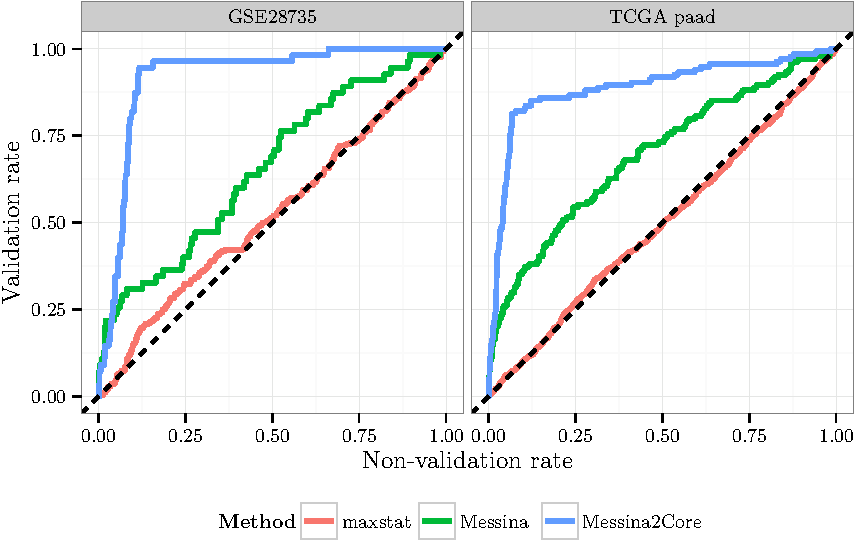
\includegraphics[width=\maxwidth]{figure/07-E3-E3-val-detcurves-plots-1} 

}



\end{knitrout}


\begin{knitrout}
\definecolor{shadecolor}{rgb}{0.969, 0.969, 0.969}\color{fgcolor}\begin{kframe}
\begin{alltt}
\hlcom{# plot(APGI.messina, indices = 1, sort_features = TRUE)}
\hlcom{# plot(APGI.messina, indices = which(APGI.feats$symbol == "IL20RB"), sort_features = FALSE)}
\hlstd{val.GSE28735.messina2[}\hlstr{"IL20RB"}\hlstd{,]}
\end{alltt}
\begin{verbatim}
##        merit threshold.train threshold.test  chisq abs.hr
## IL20RB 1.043           6.971           4.06 0.4355 0.2451
\end{verbatim}
\begin{alltt}
\hlstd{il20rb.TCGA.xc} \hlkwb{=} \hlstd{TCGA.x[}\hlstr{"IL20RB"}\hlstd{,]} \hlopt{>} \hlstd{val.TCGA.messina2[}\hlstr{"IL20RB"}\hlstd{,]}\hlopt{$}\hlstd{threshold.test}
\hlkwd{survdiff}\hlstd{(TCGA.y} \hlopt{~} \hlstd{il20rb.TCGA.xc)}
\end{alltt}
\begin{verbatim}
## Call:
## survdiff(formula = TCGA.y ~ il20rb.TCGA.xc)
## 
##                       N Observed Expected (O-E)^2/E (O-E)^2/V
## il20rb.TCGA.xc=FALSE 43       10    13.31     0.825      4.09
## il20rb.TCGA.xc=TRUE  15        7     3.69     2.978      4.09
## 
##  Chisq= 4.1  on 1 degrees of freedom, p= 0.0431
\end{verbatim}
\begin{alltt}
\hlstd{il20rb.TCGA.fit} \hlkwb{=} \hlkwd{survfit}\hlstd{(TCGA.y} \hlopt{~} \hlstd{il20rb.TCGA.xc)}
\hlkwd{print}\hlstd{(il20rb.TCGA.fit)}
\end{alltt}
\begin{verbatim}
## Call: survfit(formula = TCGA.y ~ il20rb.TCGA.xc)
## 
##                      records n.max n.start events median 0.95LCL 0.95UCL
## il20rb.TCGA.xc=FALSE      43    43      43     10    665     480      NA
## il20rb.TCGA.xc=TRUE       15    15      15      7    460     334      NA
\end{verbatim}
\begin{alltt}
\hlkwd{plot}\hlstd{(il20rb.TCGA.fit,} \hlkwc{col} \hlstd{=} \hlkwd{c}\hlstd{(}\hlstr{"red"}\hlstd{,} \hlstr{"green"}\hlstd{))}
\end{alltt}
\end{kframe}

{\centering 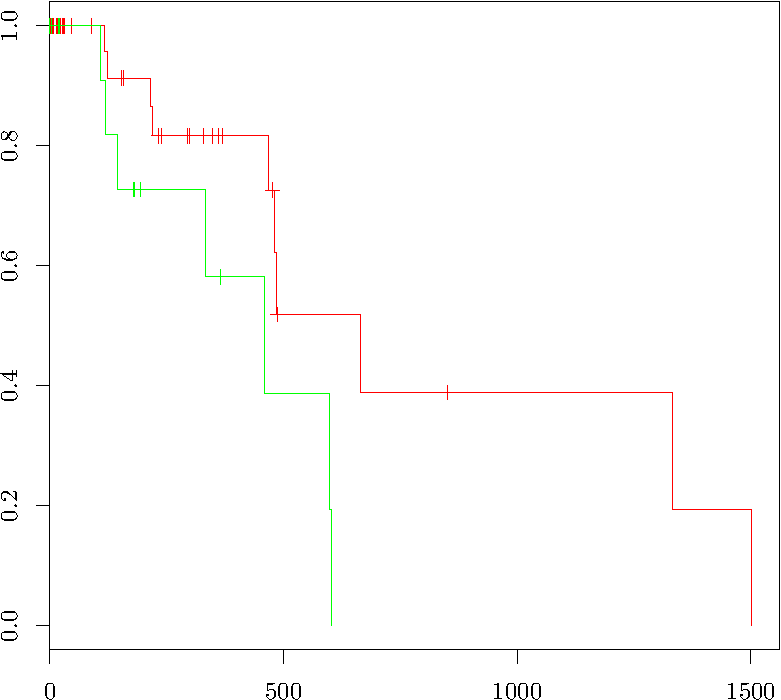
\includegraphics[width=\maxwidth]{figure/07-E3-E3-val-example-1} 

}



\end{knitrout}

\end{document}
